\mainmatter
%███████████████████████████████████████████████████████████████████
%███████████████████████████████████████████████████████████████████
%███████████████████████████████████████████████████████████████████
\chapter{Conceptual Overview}

To understand how special relativity works, we must first look at the classical understanding of the world.
Then, using the fact that light somehow always moves at a constant speed relative to everything observing it, we will see how we must change our laws of physics from the classical view for this to be true.
Which in turn will lead to many interesting consequences.
We will start with an overview of all the main concepts to understand why we need special relativity and what it means, leaving the mathematical details and deeper insights for the following chapters.

We will use all the concepts in this chapter to obtain the mathematical framework in the following chapters.
In this chapter, we will use physical objects, such as moving trains on tracks, to represent the different perspectives of various observers.
Whereas, in the mathematical chapters, we will use coordinate axes to represent the different perspectives (frames of reference).
Later, you will see the parallels between this conceptual overview and the mathematical chapters.
This chapter will provide an overview of all the required concepts for special relativity, building up the needed knowledge bit by bit, starting with our classical understanding of how perspectives (frames of reference) work and showing how our understanding must change if we are to allow all observers to view light as moving at the same constant speed.

%███████████████████████████████████████████████████████████████████
%███████████████████████████████████████████████████████████████████
\section{Classical Addition of Velocities}\label{Sect: classical velocity addition}

Let us imagine that a train is moving forward on the track at a constant speed of 20 meters per second; on the top of that train is a cannon that fires a cannonball in the direction the train is moving.
The ball travels at 100 meters per second relative to the train.
Classically, to find out how fast the ball moves relative to the track, we add the train and the ball's speed.
So, we find the ball is moving at a speed of 120 meters per second relative to the track, which is what we observe to happen.
So, in classical physics, velocities are directly added.
The ball relative to the track would move at the speed of the ball relative to the train plus the train's speed relative to the track, as shown in Figure (\ref{fig: train cannonball}).

But this turns out to just be a very good approximation for objects in our everyday life that we are used to seeing, which are moving much slower than the speed of light (roughly 300 000 000 meters per second), but we will get to this later.
For now, in the following sections, we will explain what an inertial reference frame is and how this works in the classical context so that you can see more clearly the differences between classical and special relativity.

% EDIT: change the ball's movement in the diagram
%█████████████
\begin{figure}[H]
	\figuretitle{Addition of Cannonball and Train's Velocities}
	\centering
	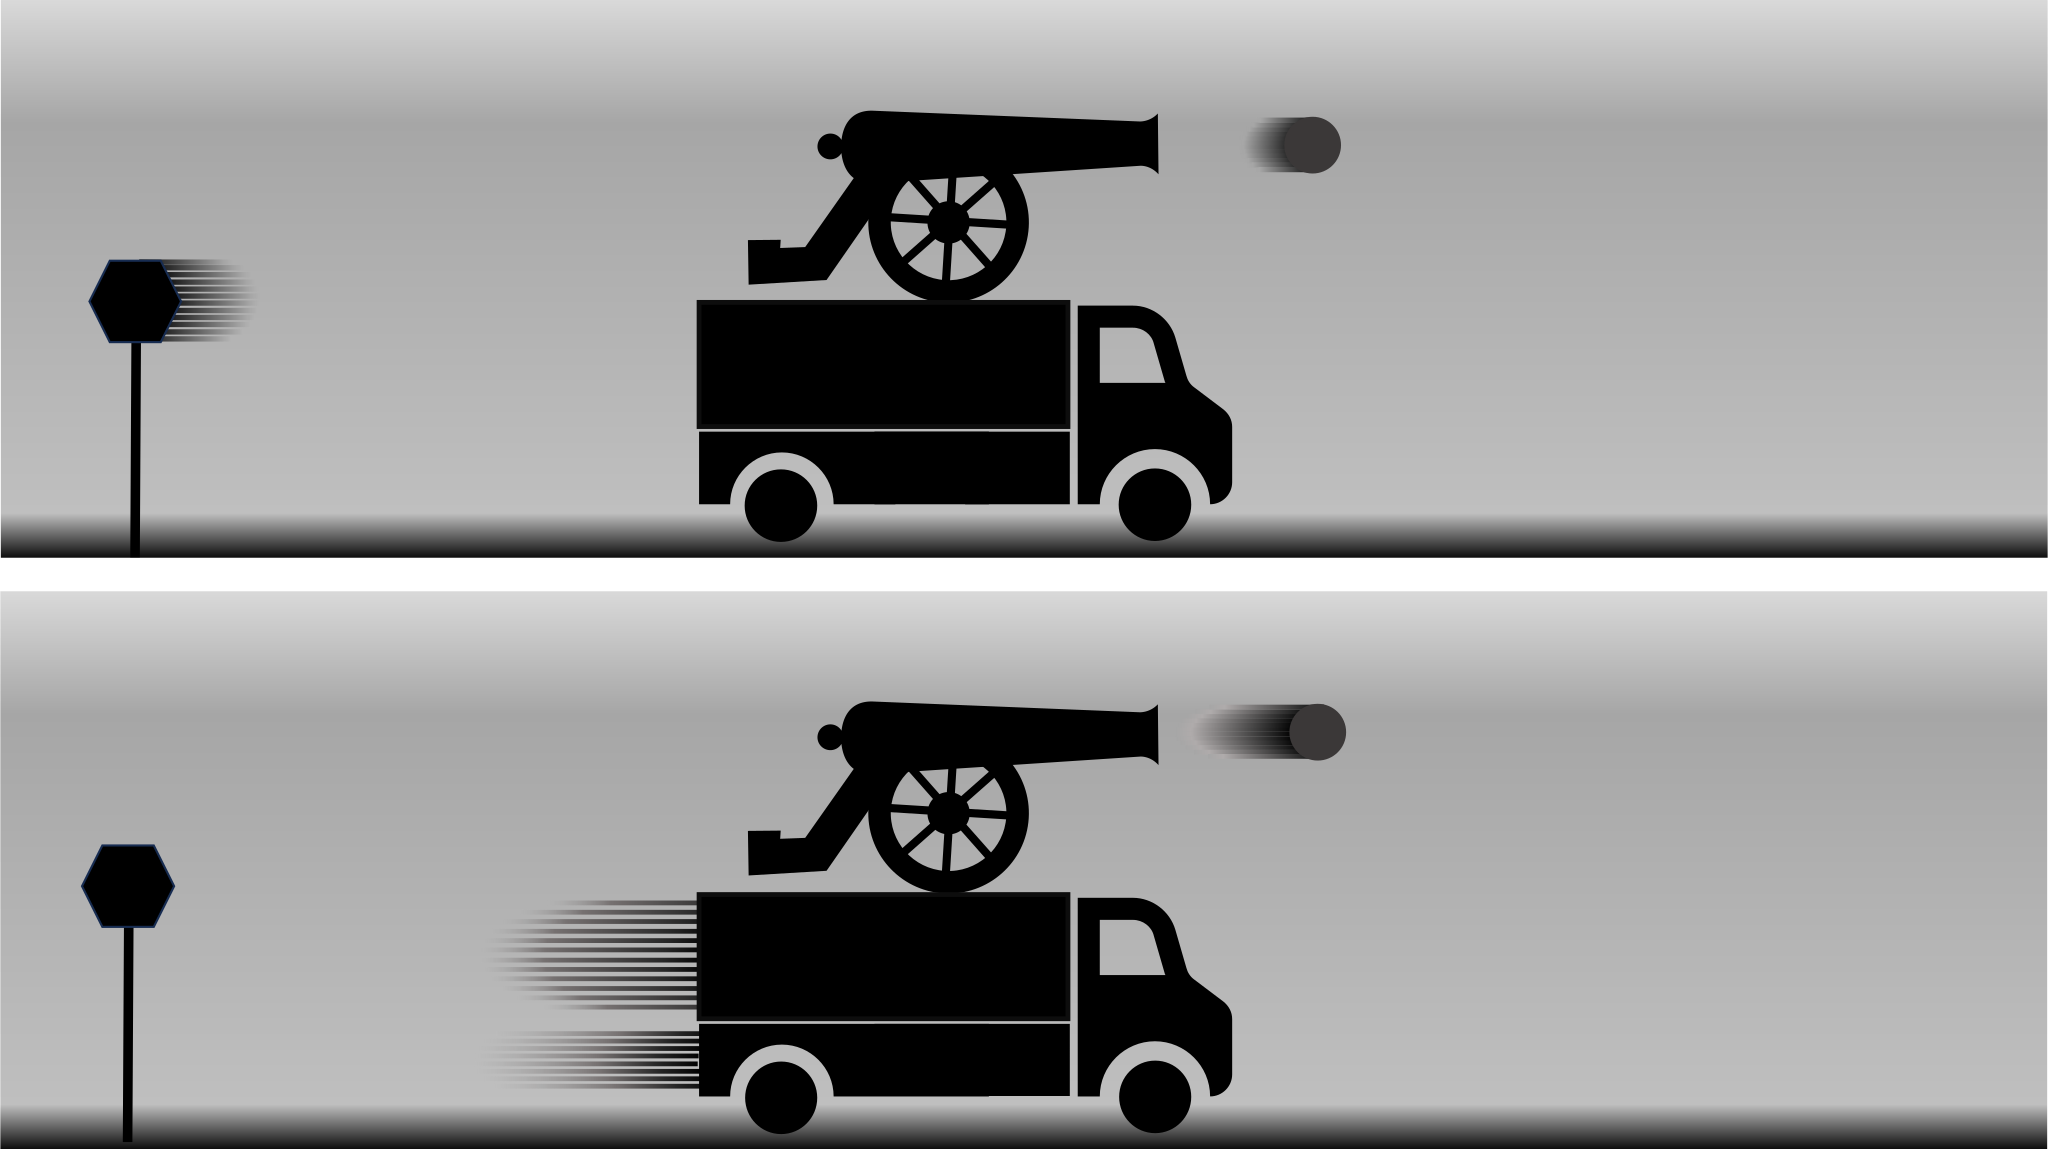
\includegraphics[width=8cm]{images/pdf/lorry_cannonball.pdf}
	\caption{A diagram, showing the speed of a cannonball from two different perspectives, (top) is from the train's perspective with the cannon at rest and the track moving backwards, the cannonball is shot and moves forward. The Figure (bottom) is from the track's perspective, with the train moving relative to it. When the cannonball is shot, it looks like it is moving forward faster, with the previous cannonball's speed combined with the speed of the cannon that it was shot from.}
	\label{fig: train cannonball}
\end{figure}
%███████████

%███████████████████████████████████████████████████████████████████
%███████████████████████████████████████████████████████████████████
\section{Inertial Reference Frame}

In the previous train example, we could associate a grid of coordinates that is stationary with respect to the train and, hence, moving along with it.
This would be the train's reference frame.
We could also associate a second grid of coordinates that are stationary with respect to the tracks, representing the track's reference frame.
These grids of coordinates are shown from the track's reference frame in Figure (\ref{fig: Reference Frames}).
%An unnecessary and more complex way of saying this is, that a \hyperlink{def-Reference-frame}{reference frame} can be thought of as an abstract coordinate system associated with an observer or object. The origin of its axis, orientation, and scale are specified by a set of points in space and their times. The purpose of it is to provide a standardized means of measuring and describing the times and positions of objects within that frame.

%Edit: make the diagram a Tikz diagram, and v in diagonal y and x direction, could also make a diagram of a grid of coordinates attached to a train moving relative to a grid of coordinates attached to the track
%█████████████
\begin{figure}[H]
	\figuretitle{Reference Frames of a Train its Track}
	\centering
	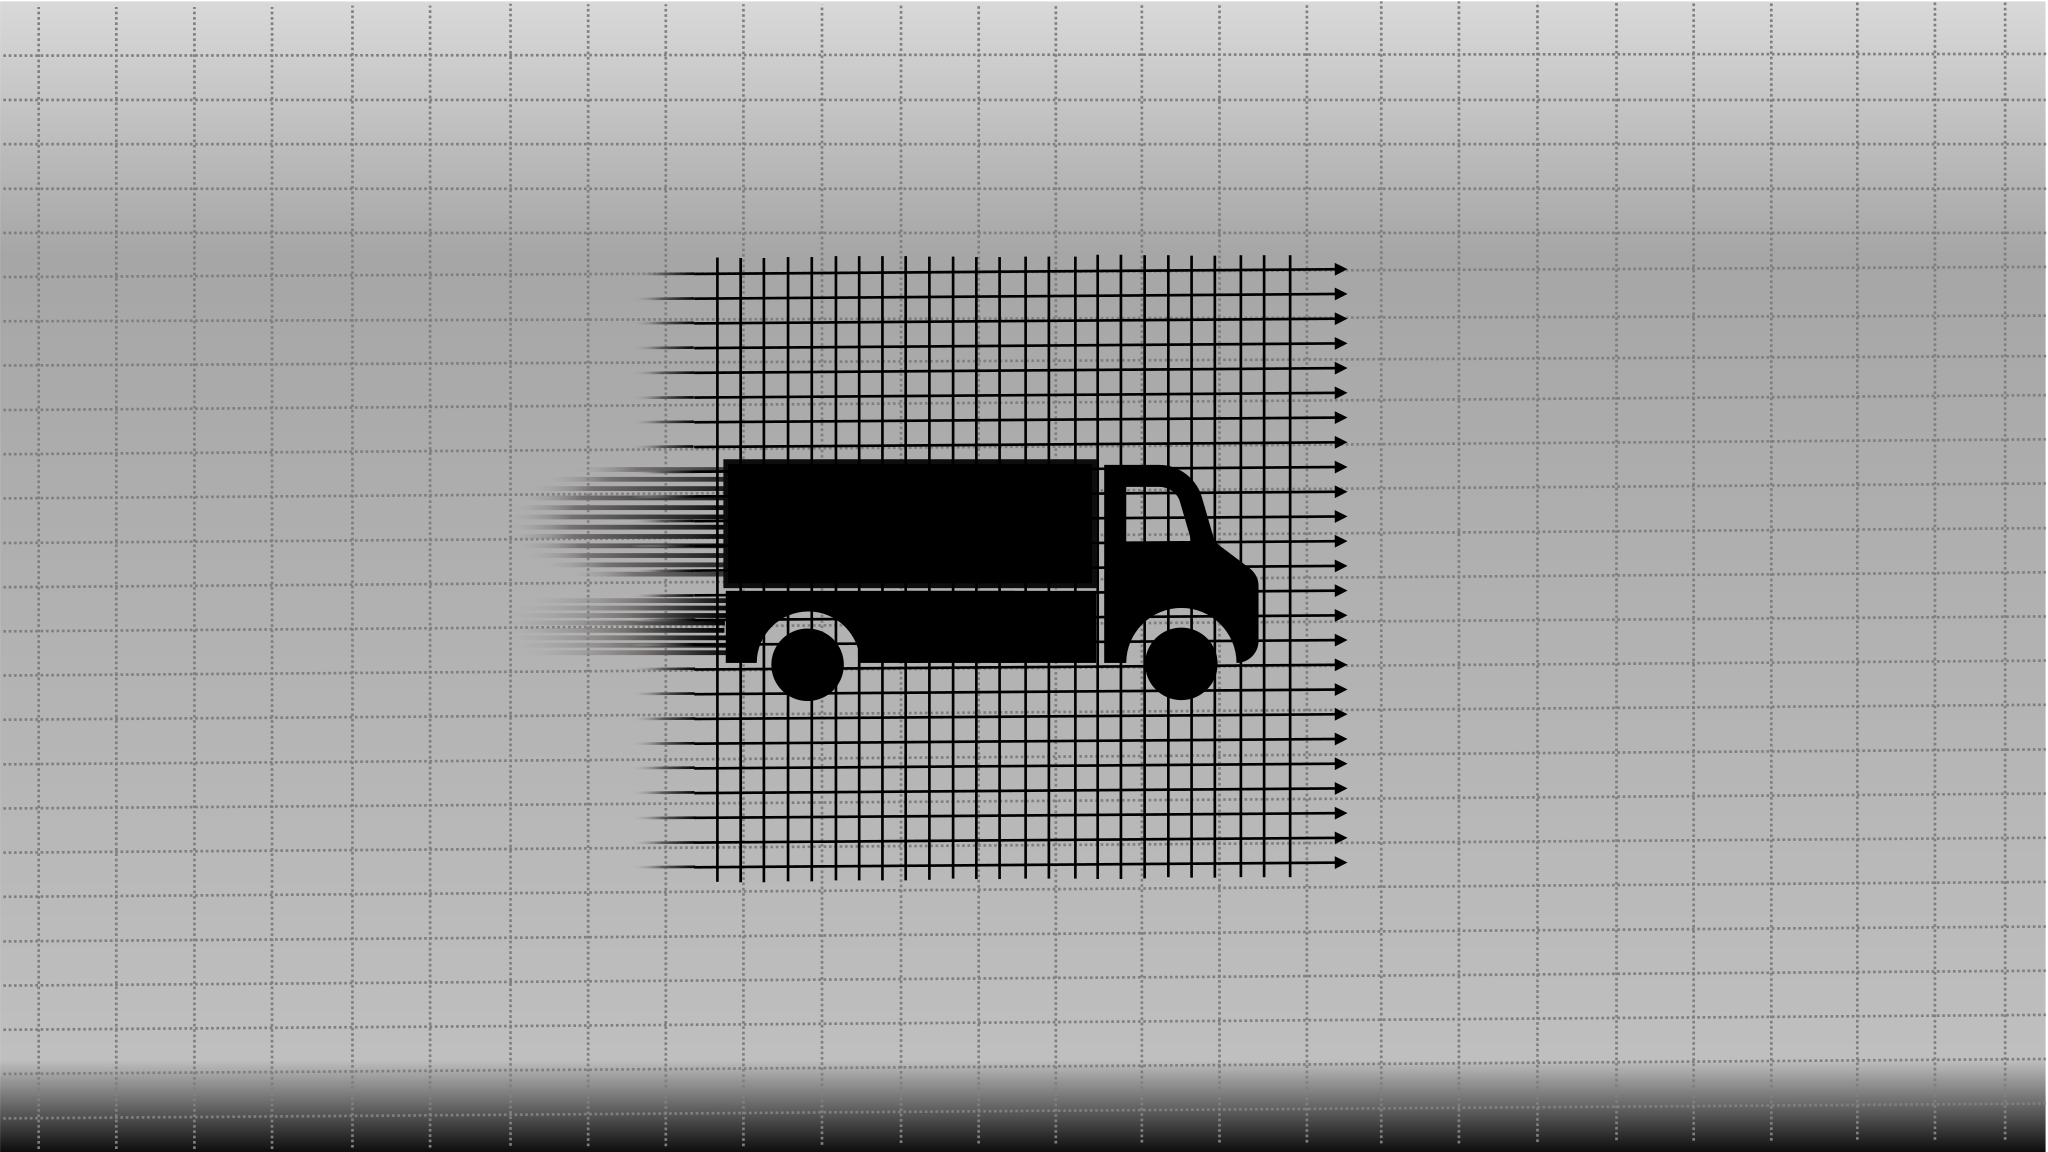
\includegraphics[width=8cm]{images/pdf/Reference_Frames_of_truck_and_road.pdf}
	\caption{A diagram, showing the \protect\hyperlink{def-Reference-frame}{reference frame} of a train as a grid of coordinates that is moving with the train relative to the tracks reference frame shown as a stationary dashed gray grid of coordinates.}
	\label{fig: Reference Frames}
\end{figure}
%███████████

An \hyperlink{def-Inertial-reference-frame}{inertial reference frame} is a reference frame that is not undergoing any acceleration.
You can tell if you are being accelerated as you will feel a force.
For example, in an accelerating car, you will feel the seat being accelerated into you, with your body slightly lagging behind in the acceleration.
This principle is used in accelerometers to measure acceleration, as shown in Figure (\ref{fig: spring boxes}).

%█████████████
\begin{figure}[H]
	\figuretitle{Inertial vs Non-Inertial Frames}
	\centering
	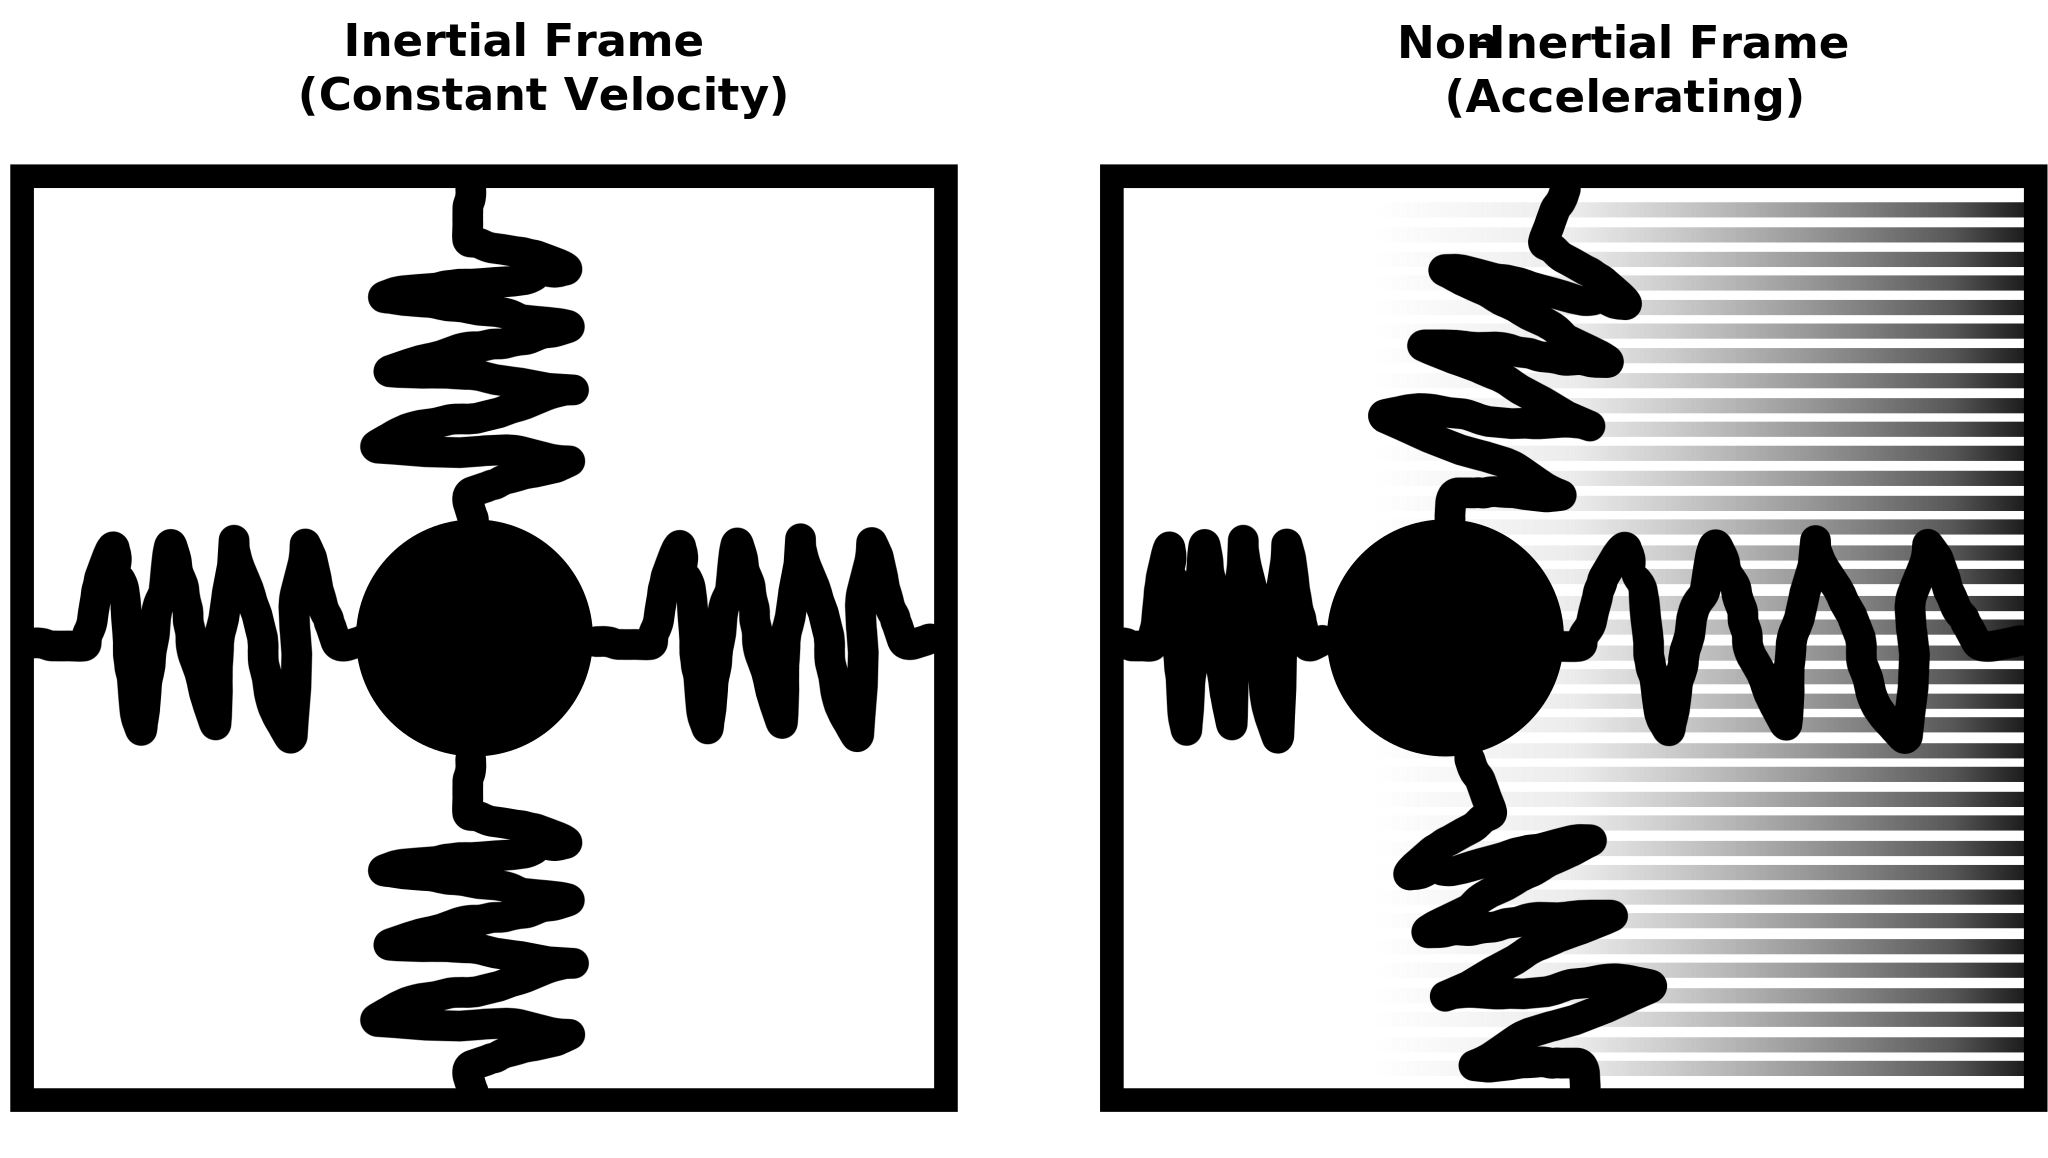
\includegraphics[width=0.9\textwidth]{images/pdf/Spring_boxes.pdf}
	\caption{A diagram, showing a ball attached to the walls of a box by springs, with the ball centered in the box in the inertial frame, with no acceleration (left), and in a non-inertial frame (right) where the box is now accelerating to the right, The ball lags behind as the box accelerates.}
	\label{fig: spring boxes}
\end{figure}
%███████████

Special relativity is just about how we change between inertial frames of reference and how it impacts the positions and the times they are at those positions.
We will now look at how movement changes in classical relativity when we change between these inertial frames.

% ((a note on free fall being inertial frame)) You may have the question of what about when the box is freefalling in gravity, and the ball would feel weightless and therefore stay in the center of the box, yet the box is accelerating, that is the beginning of general relativity which is for another handbook

%███████████████████████████████████████████████████████████████████
%███████████████████████████████████████████████████████████████████
\section{Classical Inertial Reference Frames}

To see how to swap between \hyperlink{def-Reference-frame}{reference frame}s in special relativity, we will first have to introduce what the classical swapping between two \hyperlink{def-Reference-frame}{reference frame}s looks like.

To illustrate this, we will look at a setup of two rats on a treadmill with a platform as shown in Figure (\ref{fig: 3d conveyor belt}), with three rocks hanging above the platform, which are at rest relative to the room.
The two frames of reference will be the treadmill's platform and the room in which the treadmill is in.
Both rats start under the same rock.
One rat runs to a rock positioned in the forward direction of the treadmill.
The other rat runs to an equally distanced rock to the side.
After this, they return to the starting rock.

Here, the platform can be seen as the medium in which the rats move.
Both rats travel at the same constant speed relative to the platform, with the platform either at rest or at a lower speed than the rats to allow them to get to the rocks.

%█████████████
\begin{figure}[H]
	\figuretitle{Rats on a Treadmill}
	\centering
	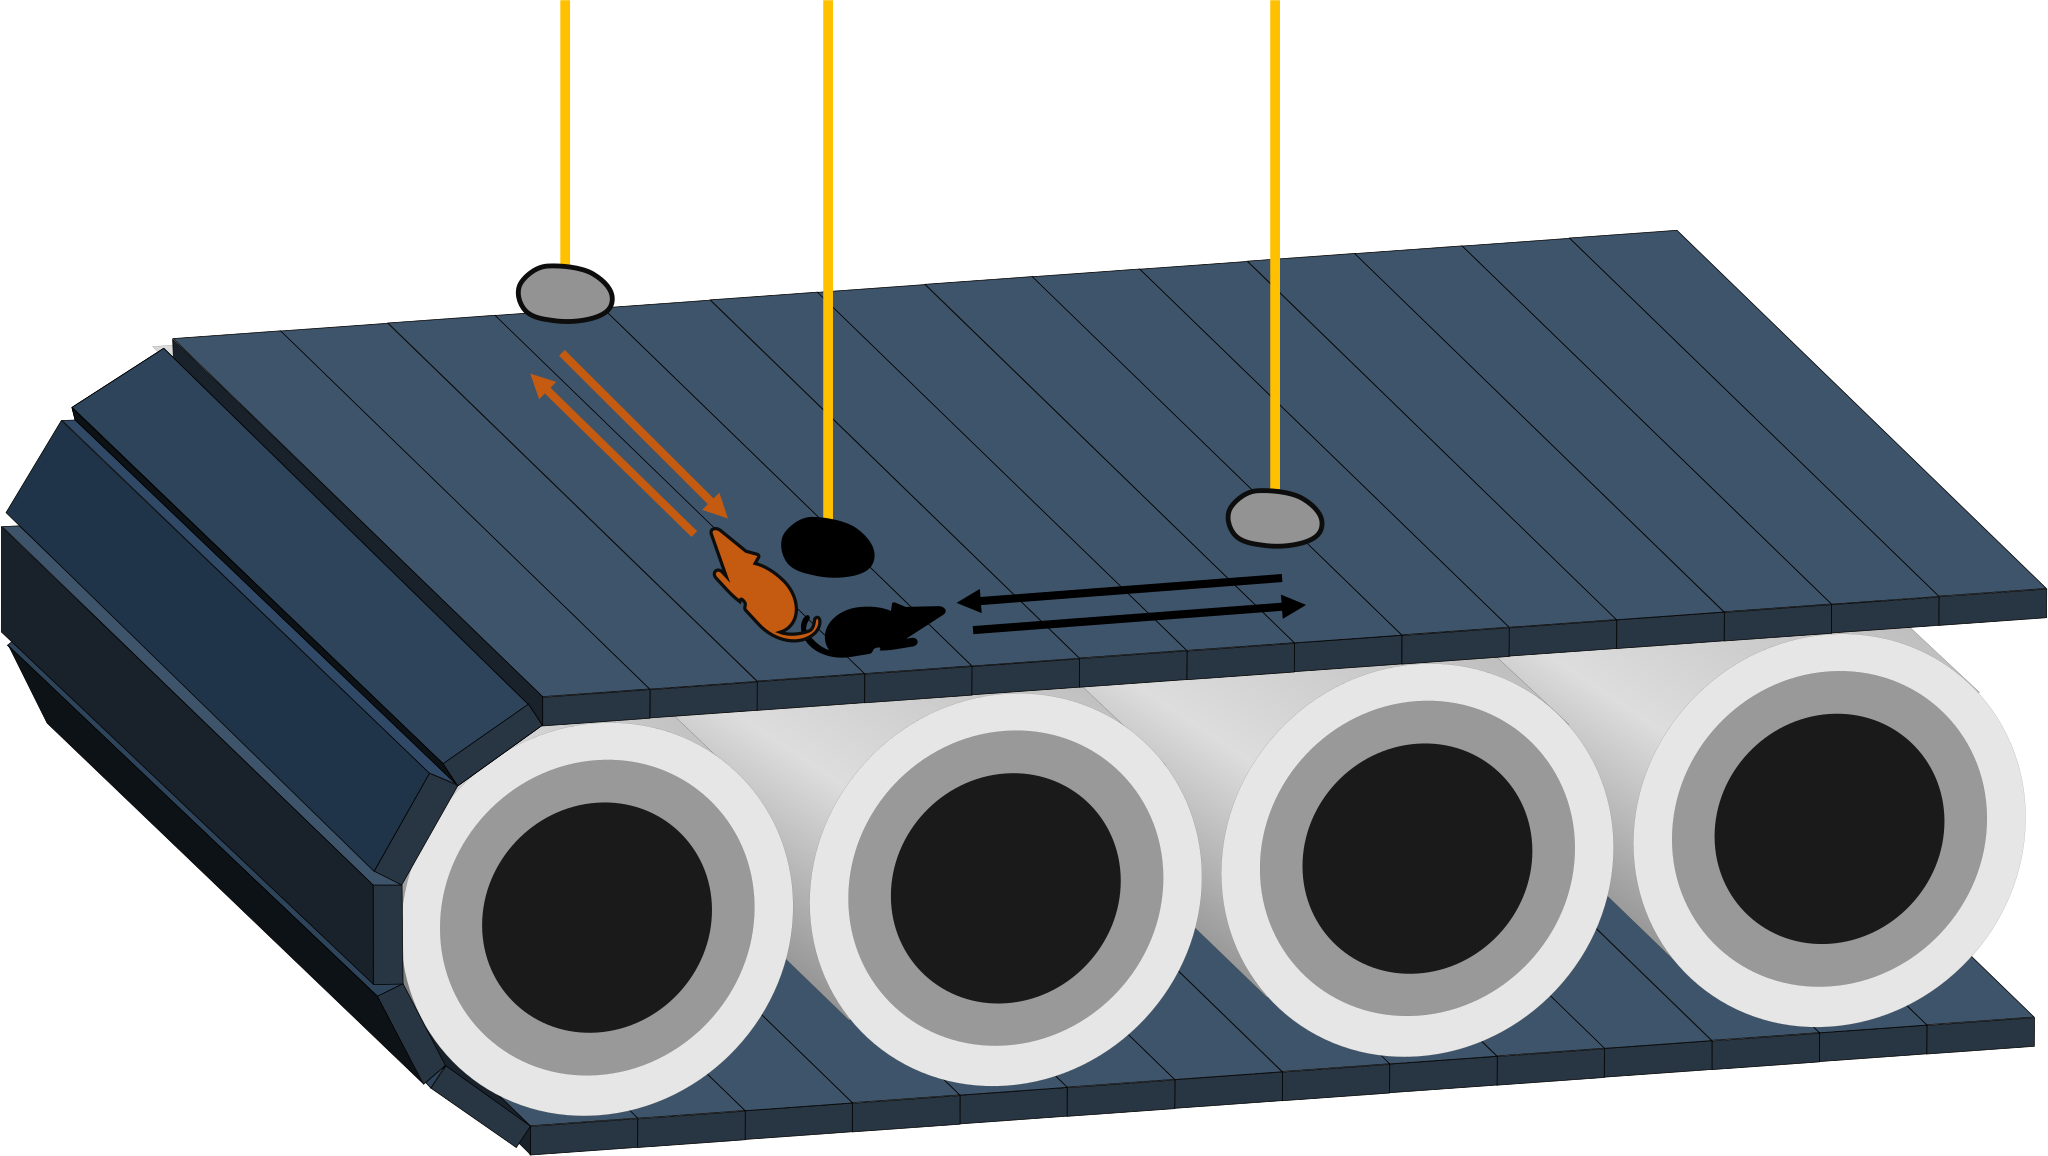
\includegraphics[width=0.9\textwidth]{images/pdf/Conveyor_belt_3d.pdf}
	\caption{A diagram, showing a 3d view of a treadmill platform, with two rats and three hanging rocks, with arrows representing the rats moving from a starting rock to the other two equally distanced rocks, with the paths perpendicular to each other.}
	\label{fig: 3d conveyor belt}
\end{figure}
%███████████

If the platform is at rest, they will return to the starting rock simultaneously.
But if the treadmill is turned on and the platform is moving, the rats will also have to work against the movement of the platform to get to the rocks.
This will lead to different distances the rats have to travel relative to the platform, and as a result, the rats get back to the starting rock at different times.
Figure (\ref{fig: treadmill}) shows what the direction of movement of the rats and rocks look like in each of the \hyperlink{def-Reference-frame}{reference frame}s when the platform is moving.

%█████████████
\begin{figure}[H]
	\figuretitle{Different Reference Frames of Rats on Treadmill}
	\centering
	\begin{subfigure}{0.9\textwidth}
		\centering
		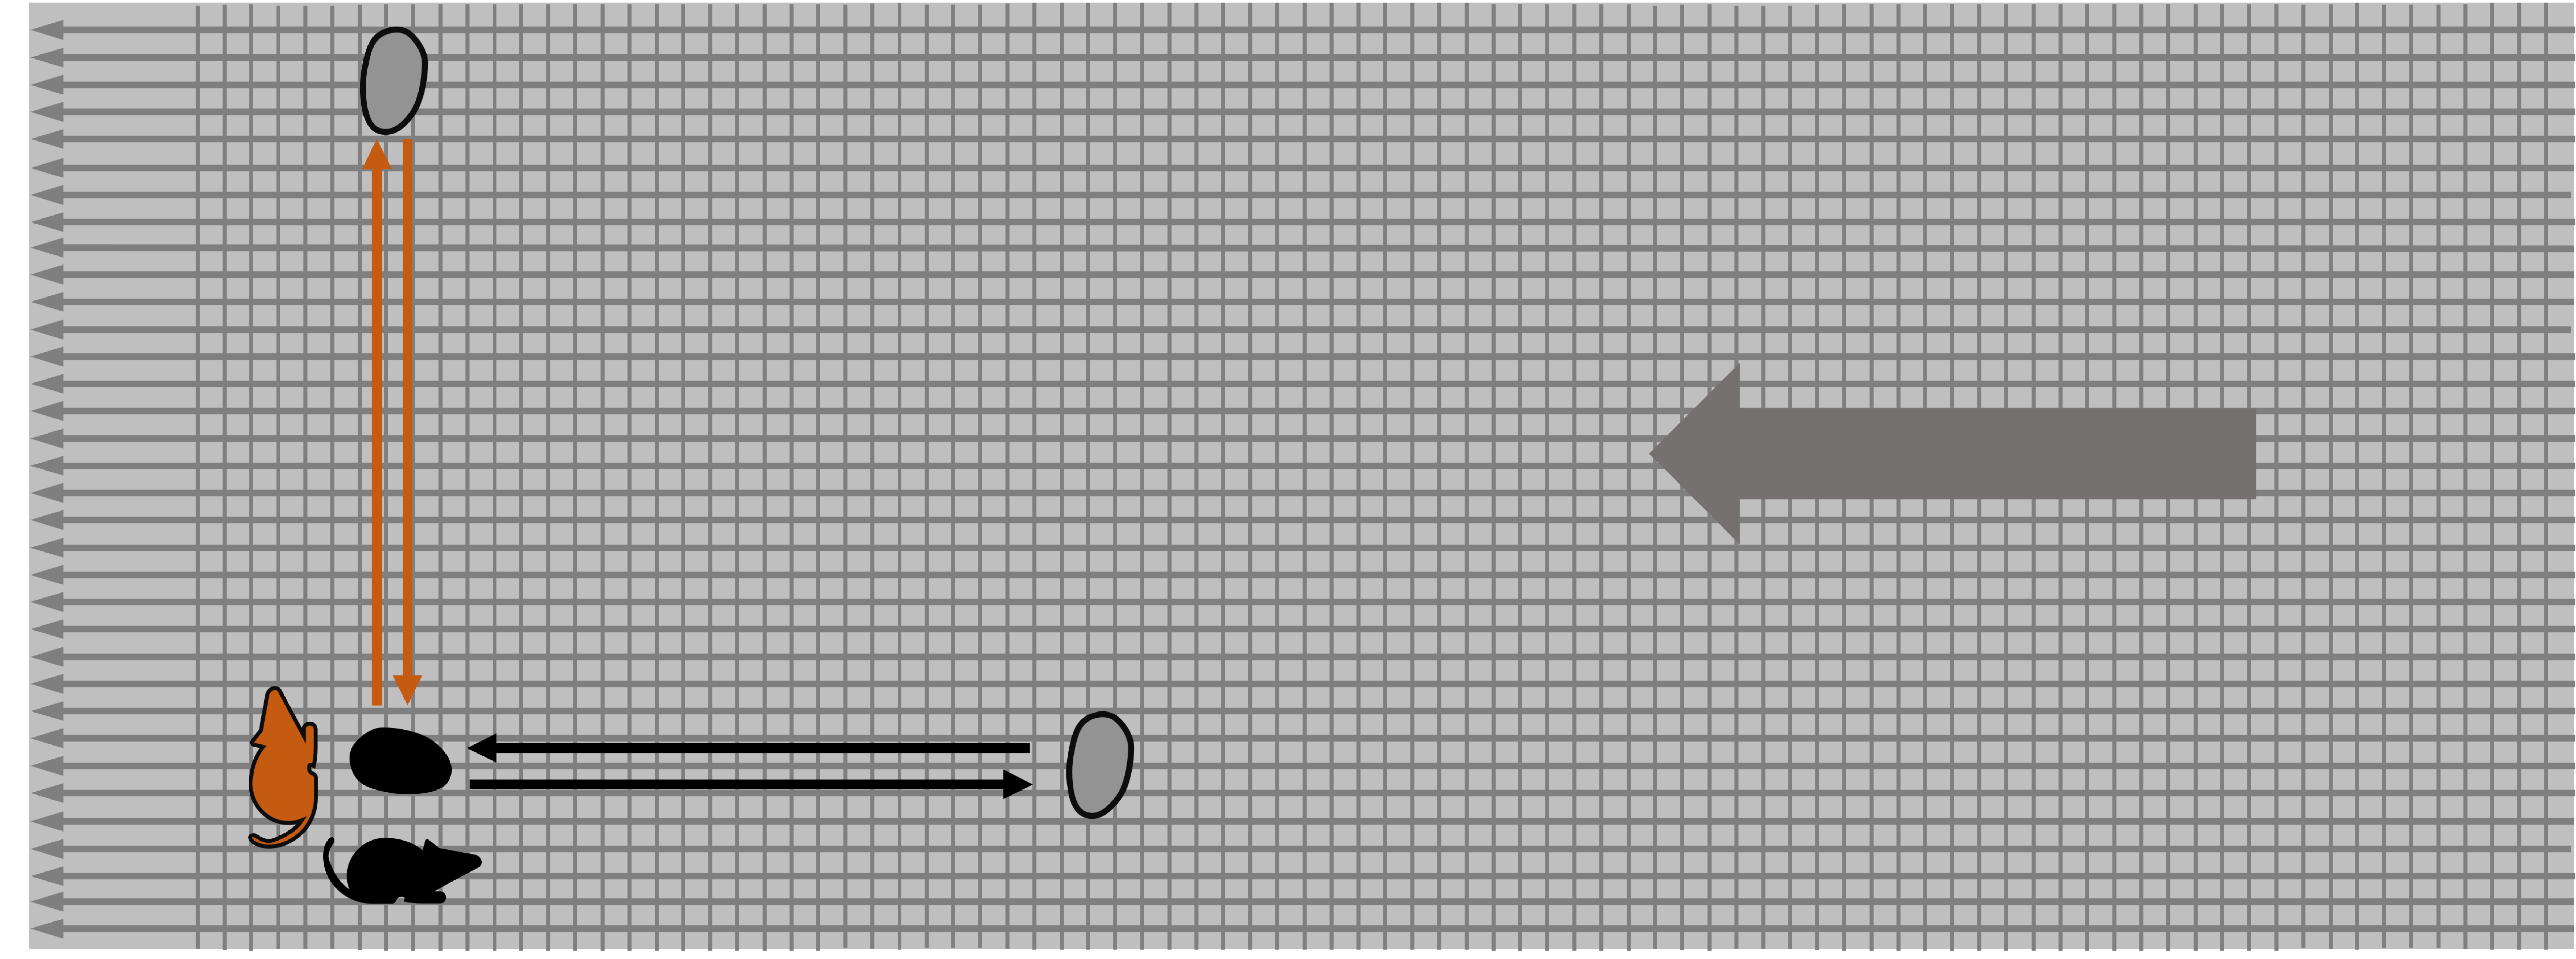
\includegraphics[width=\textwidth]{images/pdf/rats_moving.pdf}
		\caption{Room's \protect\hyperlink{def-Reference-frame}{reference frame}.}
		\label{fig: rat with moving platform}
	\end{subfigure}
	\begin{subfigure}{0.9\textwidth}
		\vspace{0.2cm}
		\centering
		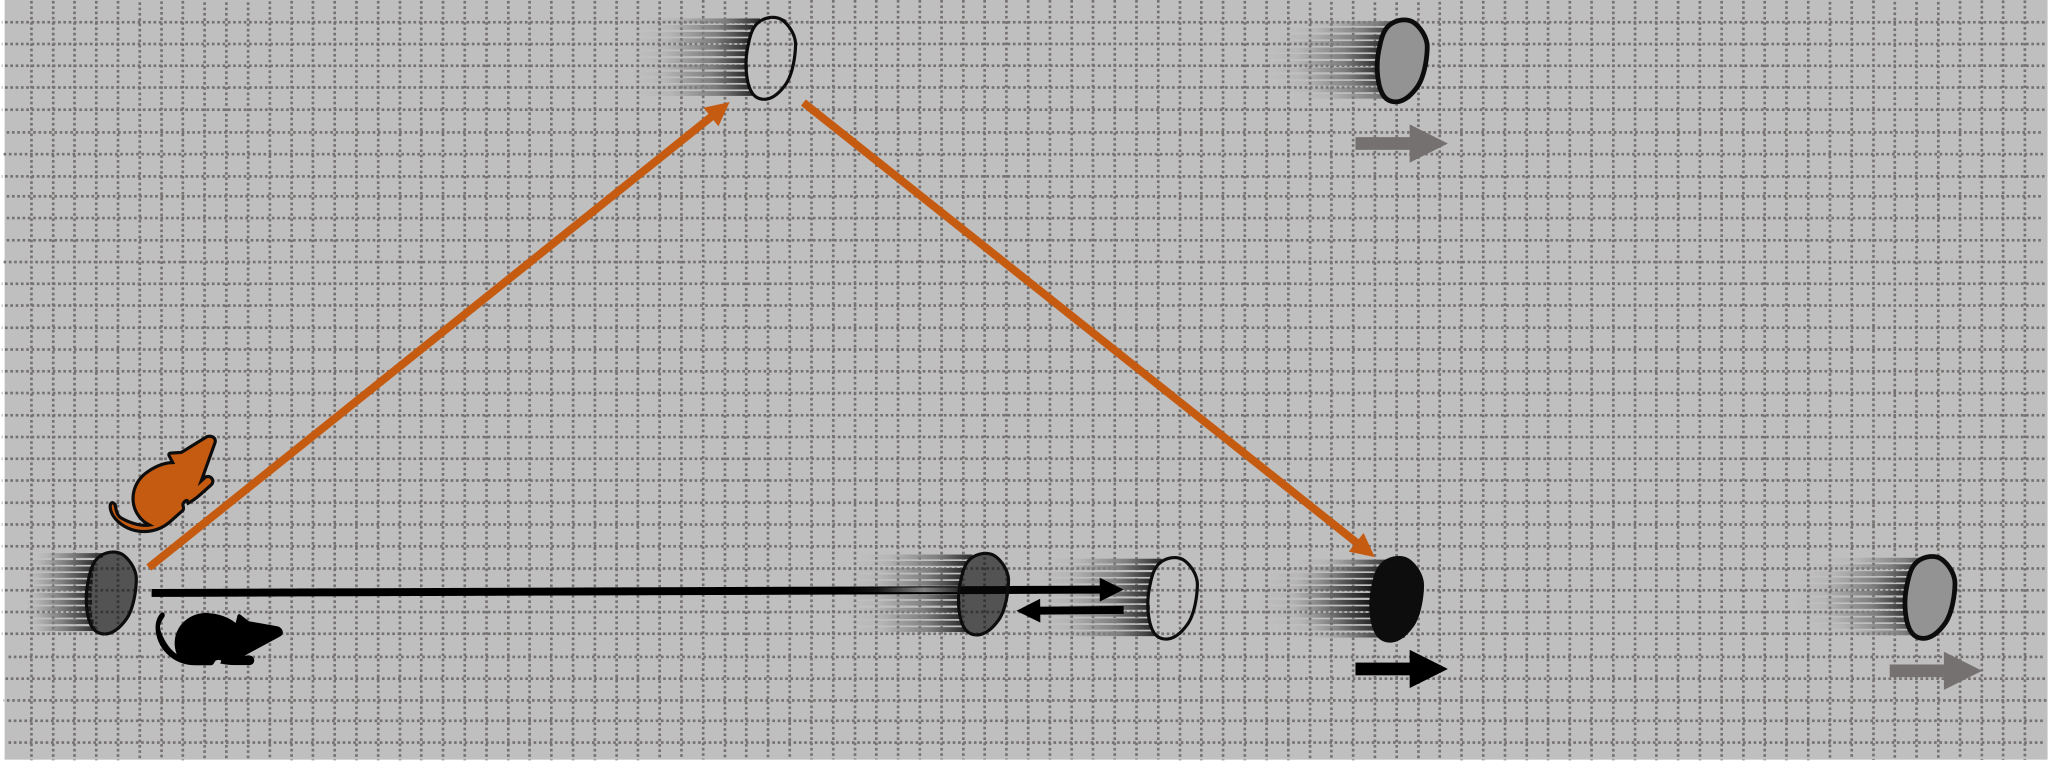
\includegraphics[width=\textwidth]{images/pdf/rats_platform_frame.pdf}
		\caption{Platform's \protect\hyperlink{def-Reference-frame}{reference frame}.}
		\label{fig: rat platform reference frame}
	\end{subfigure}
	\caption{Rats running on a moving platform of a treadmill from two different \protect\hyperlink{def-Reference-frame}{reference frame}s, with the paths of the rats represented as arrows.}
	\label{fig: treadmill}
\end{figure}
%███████████

\iffalse javascript{rats_on_treadmill}
\fi

In the room's \hyperlink{def-Reference-frame}{reference frame}, we have the platform moving backwards.
The rat that is moving straight ahead will have impedance to its movement from the backwards pull of the platform.
But after it turns around, it will have a boost from the platform to return to the starting rock.
Meanwhile, the sideways-moving rat will have to move sideways and balance out the platform's backwards pull to keep its movement in the direction of the hanging rocks.
This gives different lengths of paths depending on the \hyperlink{def-Reference-frame}{reference frame}, as shown in Figure (\ref{fig: treadmill}).
The rats in the platform's reference frame, move with the same speed for all the paths, represented by the arrows.
Whereas, in the room's reference frame, we have a slower constant speed of the sideways-moving rat and two different speeds for the forward and backward paths of the other rat.
This leads to different times for the rats to return to the starting rock.

The rats here use the medium of the treadmill's platform to move, and similarly, it was thought that light needed a medium, called the aether, to travel through space.
If there was this medium, we could test how fast it moved relative to Earth by finding the difference between the return times of light emitted in two perpendicular directions, just as in the treadmill example.
So, next, we will look at the notion of a universal medium referred to as the \hyperlink{def-aether}{aether} and whether we can have the same frame swapping when it comes to light traveling in two different frames of reference, as we did in this section.

%███████████████████████████████████████████████████████████████████
%███████████████████████████████████████████████████████████████████
\section{The Aether}%, a Medium for Light} % and a Universal Rest Frame}

In the 1800s, the theory was that light was a wave and, therefore, would need a medium that filled the \hyperlink{def-vacuum}{vacuum} of space for it to travel through, called "the luminiferous \hyperlink{def-aether}{aether}", and that light would travel at a constant speed relative to this \hyperlink{def-aether}{aether}, like how the rats in the previous section moved at a constant speed relative to the medium of the treadmill's platform.
If the aether existed, the Earth would be moving through it, illustrated in Figure (\ref{fig: Aether}).

%█████████████
\begin{figure}[ht]
	\figuretitle{The Earth and the Aether}
	\centering
	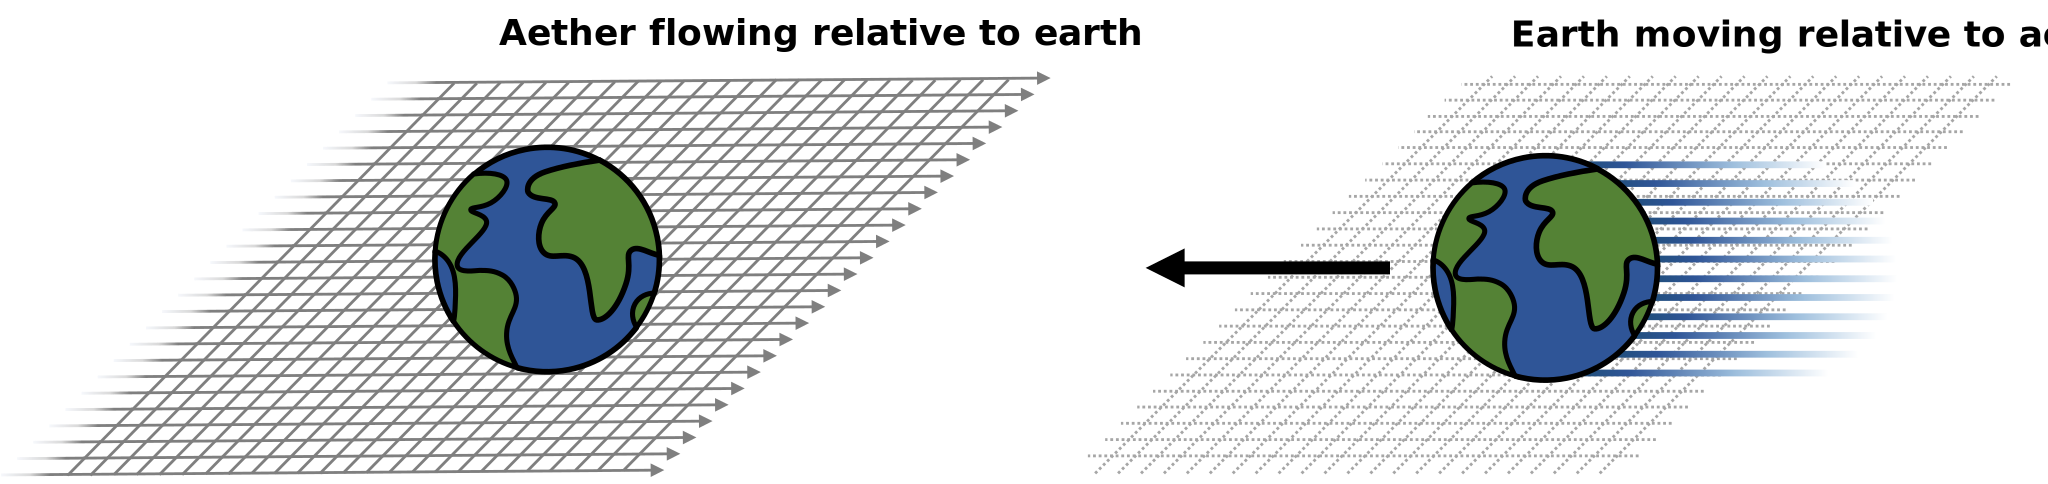
\includegraphics[width=0.9\textwidth]{images/pdf/earth_and_aether.pdf}
	\caption{A diagram showing the proposed \protect\hyperlink{def-aether}{aether}'s and Earth's movement relative to each other.}
	\label{fig: Aether}
\end{figure}
%███████████

So, an experimental setup by Michelson and Morley, shown in Figure (\ref{fig: Michelson_morley}), called an interferometer, was devised to measure Earth's movement through the \hyperlink{def-aether}{aether} \cite{EtherExperiment}, by measuring how it affected the return times of light that were emitted in different directions, as observed in Earth's \hyperlink{def-Reference-frame}{reference frame}.
It did this by splitting a single light beam into two perpendicular paths that are then reflected back to be recombined and sent toward a light detector.
By rotating the setup, the two light paths could be aligned, one parallel and the other perpendicular to the Earth's motion through the presumed \hyperlink{def-aether}{aether}.
They reasoned that if the speed of light was constant with respect to the proposed \hyperlink{def-aether}{aether}, just like in the rat experiment from the previous section, the split light beams would recombine at different times.

From the previous section's system of rats on a treadmill, we can see that the treadmill's platform is analogous to the \hyperlink{def-aether}{aether}, and the rats are analogous to the light.
Both have the room where these experiments are done as the other inertial reference frame.

%█████████████
\begin{figure}[H]
	\figuretitle{Experiment to Detect the Aether}
	\centering
	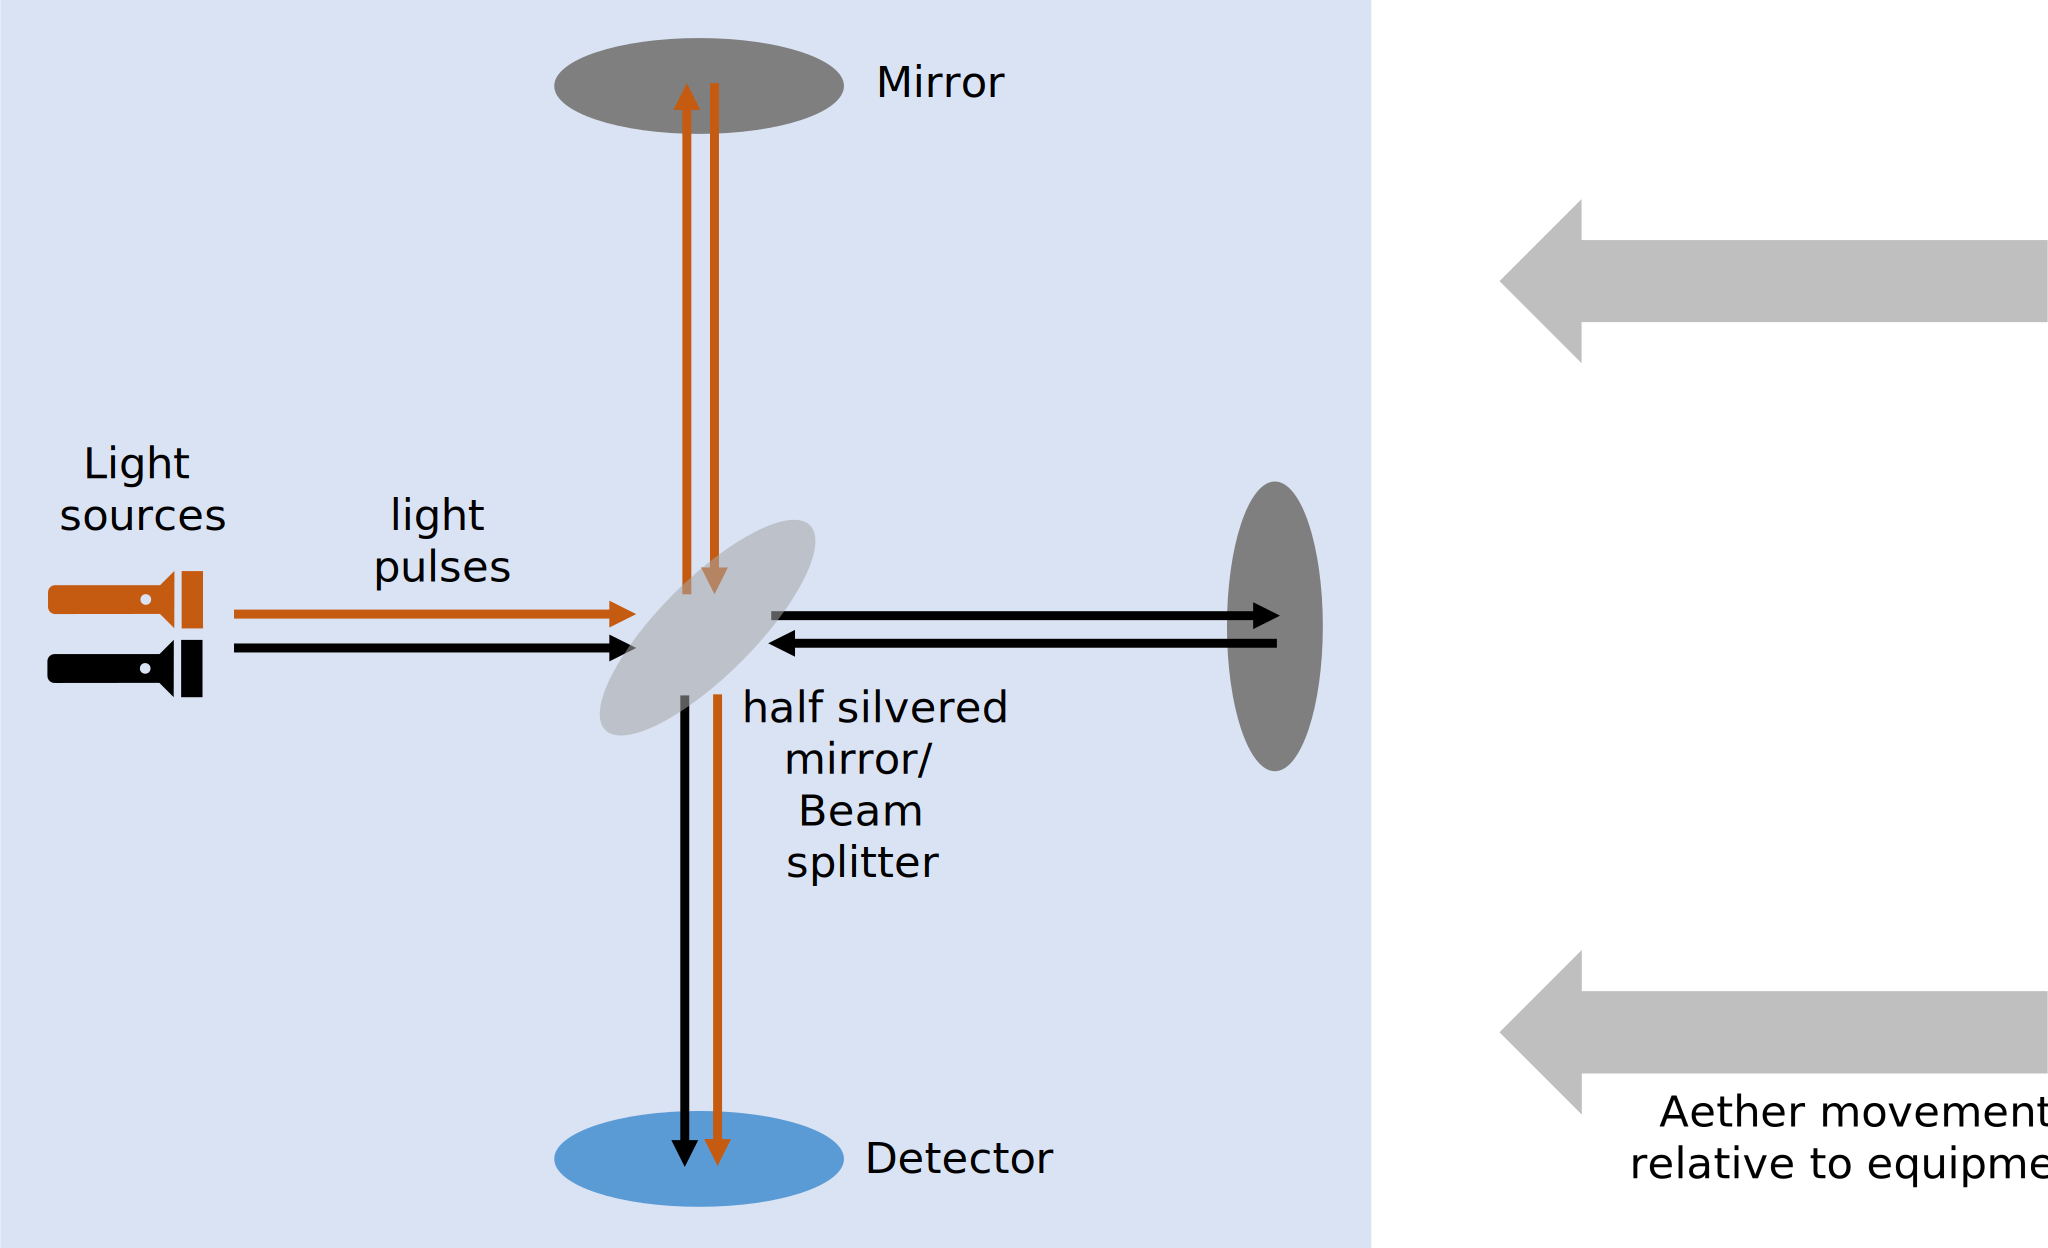
\includegraphics[width=8cm]{images/pdf/Michelson_morley.pdf}
	\caption{A diagram showing the Michelson-Morley experiment, we can take the part of the paths between the beam splitter and two mirrors to be analogous to the case of the paths in the previous section of the rat and treadmill system.}
	\label{fig: Michelson_morley}
\end{figure}
%███████████

However, when Michelson and Morley performed the experiment, they found no difference in travel time to the detector for both paths, indicating that there was no difference in the speed of light in any direction in Earth's \hyperlink{def-Reference-frame}{reference frame}.
Hence, light's speed is not dependent on the supposed \hyperlink{def-aether}{aether}.
This null result seriously discredited the \hyperlink{def-aether}{aether} theories.
It ultimately led to the proposal by Einstein in 1905 that the speed of light (in a \hyperlink{def-vacuum}{vacuum}) is a universal constant and is independent of the motion of the \hyperlink{def-observer}{observer} or source.

To allow for us to have this universal speed of light (in a \hyperlink{def-vacuum}{vacuum}), it will require us to change our ideas of how time and positions are perceived by different \hyperlink{def-observer}{observer}s.

%███████████████████████████████████████████████████████████████████
%███████████████████████████████████████████████████████████████████
\section{Speed of Light}% as a Constant}

The experiments showed light does not have a medium that it travels at a constant velocity relative to and, therefore, must instead travel at a constant velocity in a \hyperlink{def-vacuum}{vacuum} in all \hyperlink{def-Reference-frame}{reference frame}s.
This is independent of how fast the source and receiver of that light are moving in the frame, as shown with a moving train's headlights in Figure (\ref{fig: train torch}).
Light moves slower in objects such as glass, but this is due to the interactions between it and the material, impeding the movement of light.

Light itself moves extremely fast compared to any other everyday speeds we are used to (roughly 300 000 000 meters per second; it can travel the world's diameter in the blink of an eye).
This is why we do not notice any delay in things we see in everyday life, though we should remember that there is this delay.
For example, the light we currently see from the sun was emitted eight minutes ago for it to reach us now, and the further an object is located from us, the further back in time we are currently seeing it because of this delay.

When we look at the same train setup as in Figure (\ref{fig: train cannonball}), but now have it in a \hyperlink{def-vacuum}{vacuum}, where the cannon firing a cannonball is swapped for headlights emitting light, we will find the same speed of light when measured relative to the train or the track, but how can this be true?

%█████████████
\begin{figure}[H]
	\figuretitle{Emitted Light in Different Frames}
	\centering
	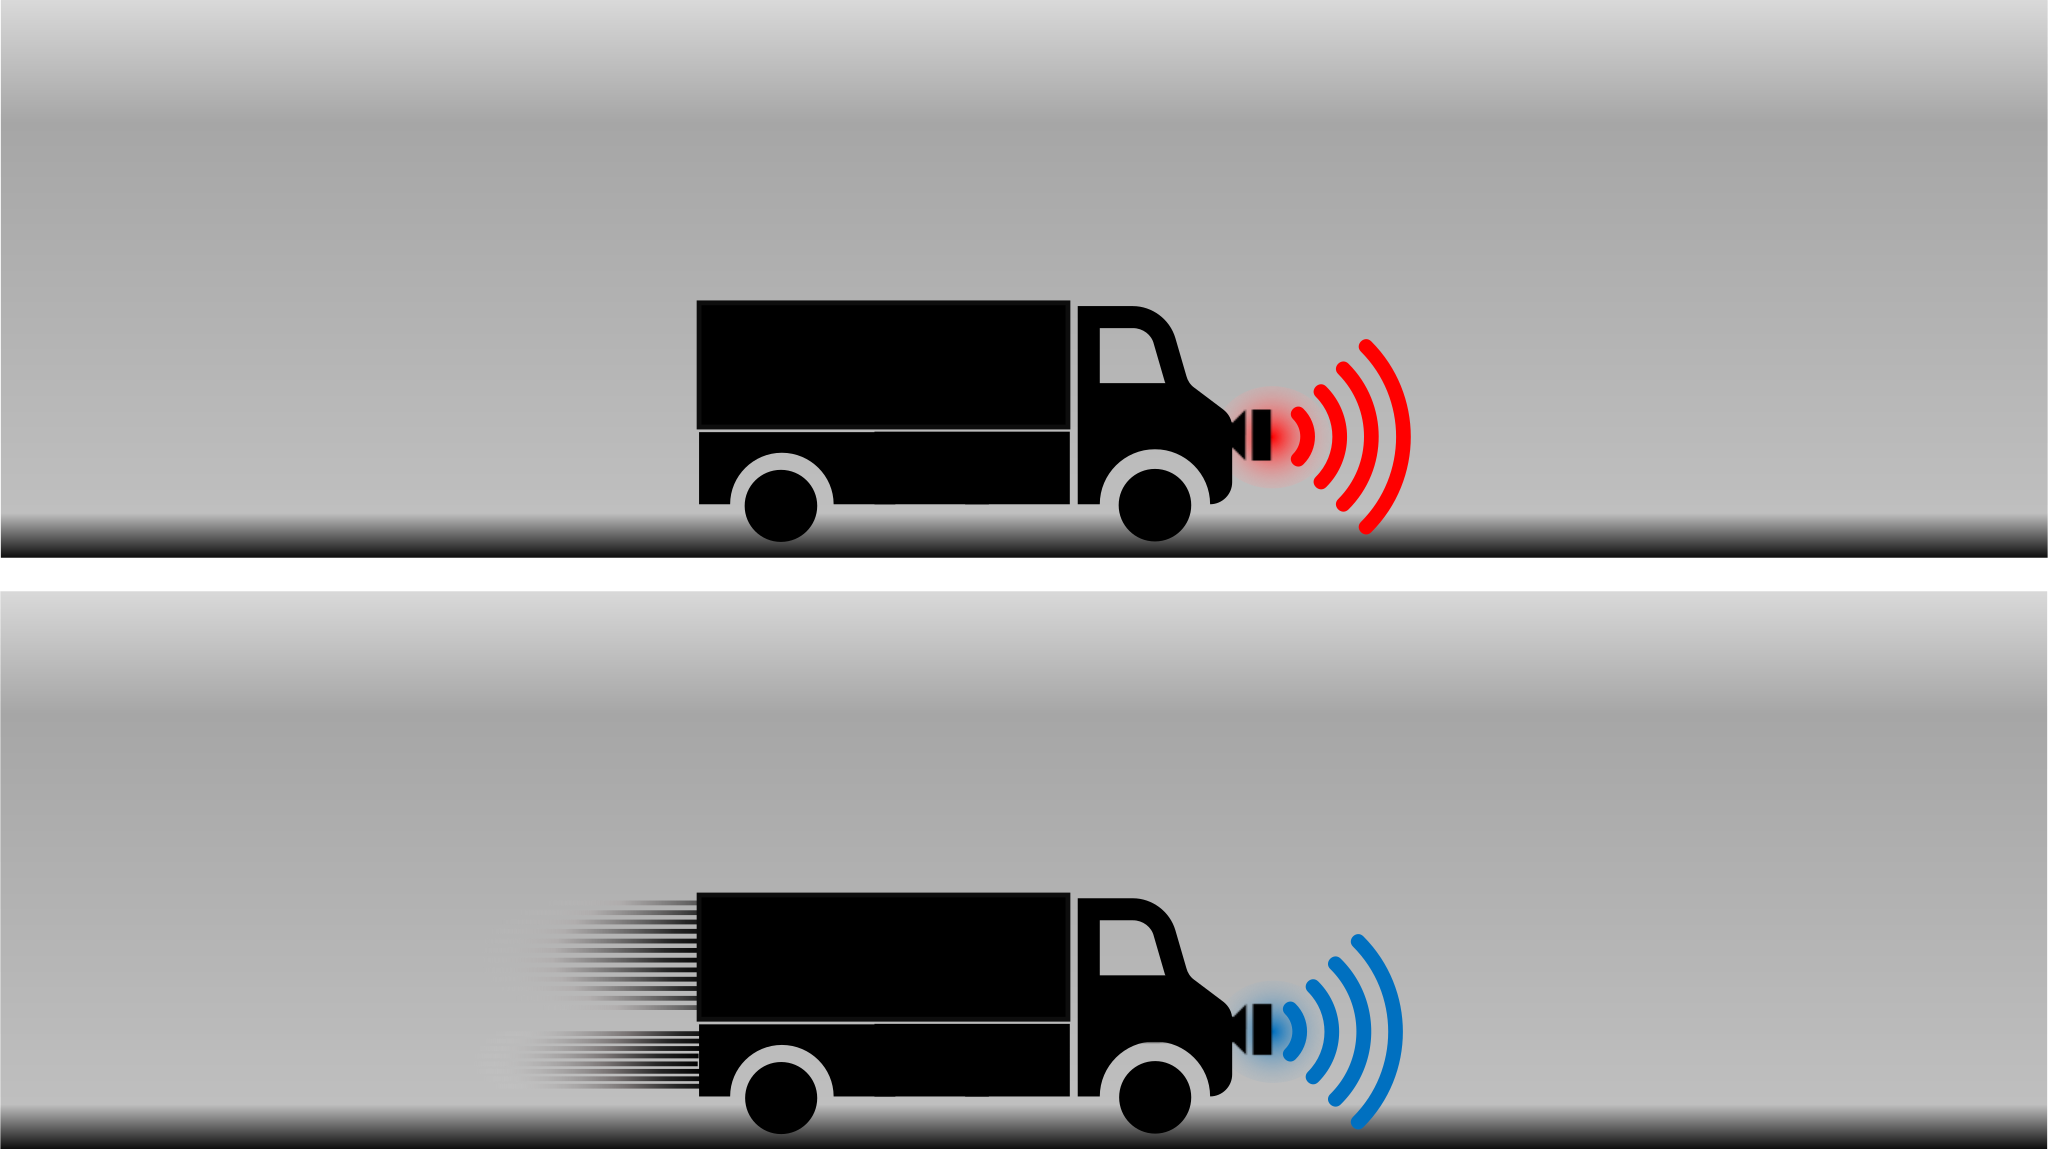
\includegraphics[width=8cm]{images/pdf/lorry_torch.pdf}
	\caption{A diagram, showing light emitted from a train in two different \protect\hyperlink{def-Reference-frame}{reference frame}s, with the emitted light having the same speed in each frame, though with different frequencies and energies due to the \protect\hyperlink{def-doppler-effect}{Doppler effect}, which will be explained later.}
	\label{fig: train torch}
\end{figure}
%███████████

For this to be true, we need a new way of thinking about velocity addition.
This is because the velocities of objects must be added in a way that is consistent with the requirement that the speed of light is constant but also gives the approximate classical addition at speeds of objects at much less than the speed of light, like how we observed in the situation with the cannon and train, shown in Figure (\ref{fig: train cannonball}).
Since the speed of the light depends only on the units of time and positions, the only way to correct for this is to have the measured positions and times of objects \hyperlink{def-transform}{transform} differently when swapping between \hyperlink{def-Reference-frame}{reference frame}s than the classical way.
This is what we will talk about next.
For the curious, it was the \href{https://scienceready.com.au/pages/determination-of-speed-of-light}{experiment by Ole Rømer} that showed that light traveled at a finite speed rather than being instantaneously emitted and received.

%███████████████████████████████████████████████████████████████████
%███████████████████████████████████████████████████████████████████
\section{Position and Time}

%███████████████████████████████████████████████████████████████████
\subsection{Time Dilation}\label{Subsect: Time Dilation}

Let us imagine a simple clock, as shown in Figure (\ref{fig: train clock}), made of a light pulse moving back and forth between two mirrors on a moving train's floor and roof.
We will keep time by taking a tick of this clock to be when the light travels from one mirror to the other and back again.
For an \hyperlink{def-observer}{observer} in the train, they will see the light go straight up and down between the mirrors, but an \hyperlink{def-observer}{observer} stationary relative to the track will see not just the light traveling up and down but also with the direction of the train.
Hence, it will travel a longer distance between ticks.

Since the distance traveled by the light in the moving frame is longer and the speed of light is the same for both reference frames, as shown in previous sections, we are only left with two possibilities to keep the speed of light invariant: either the height of the train is shorter, to give the same path length for light so that the ticks happen at the same rate, or that time itself moves slower in moving objects, the first option leads to paradoxes as shown in Figure (\ref{fig: width contraction}).

%█████████████
\begin{figure}[H]
	\figuretitle{Paradox of Height and Width Contraction}
	\centering
	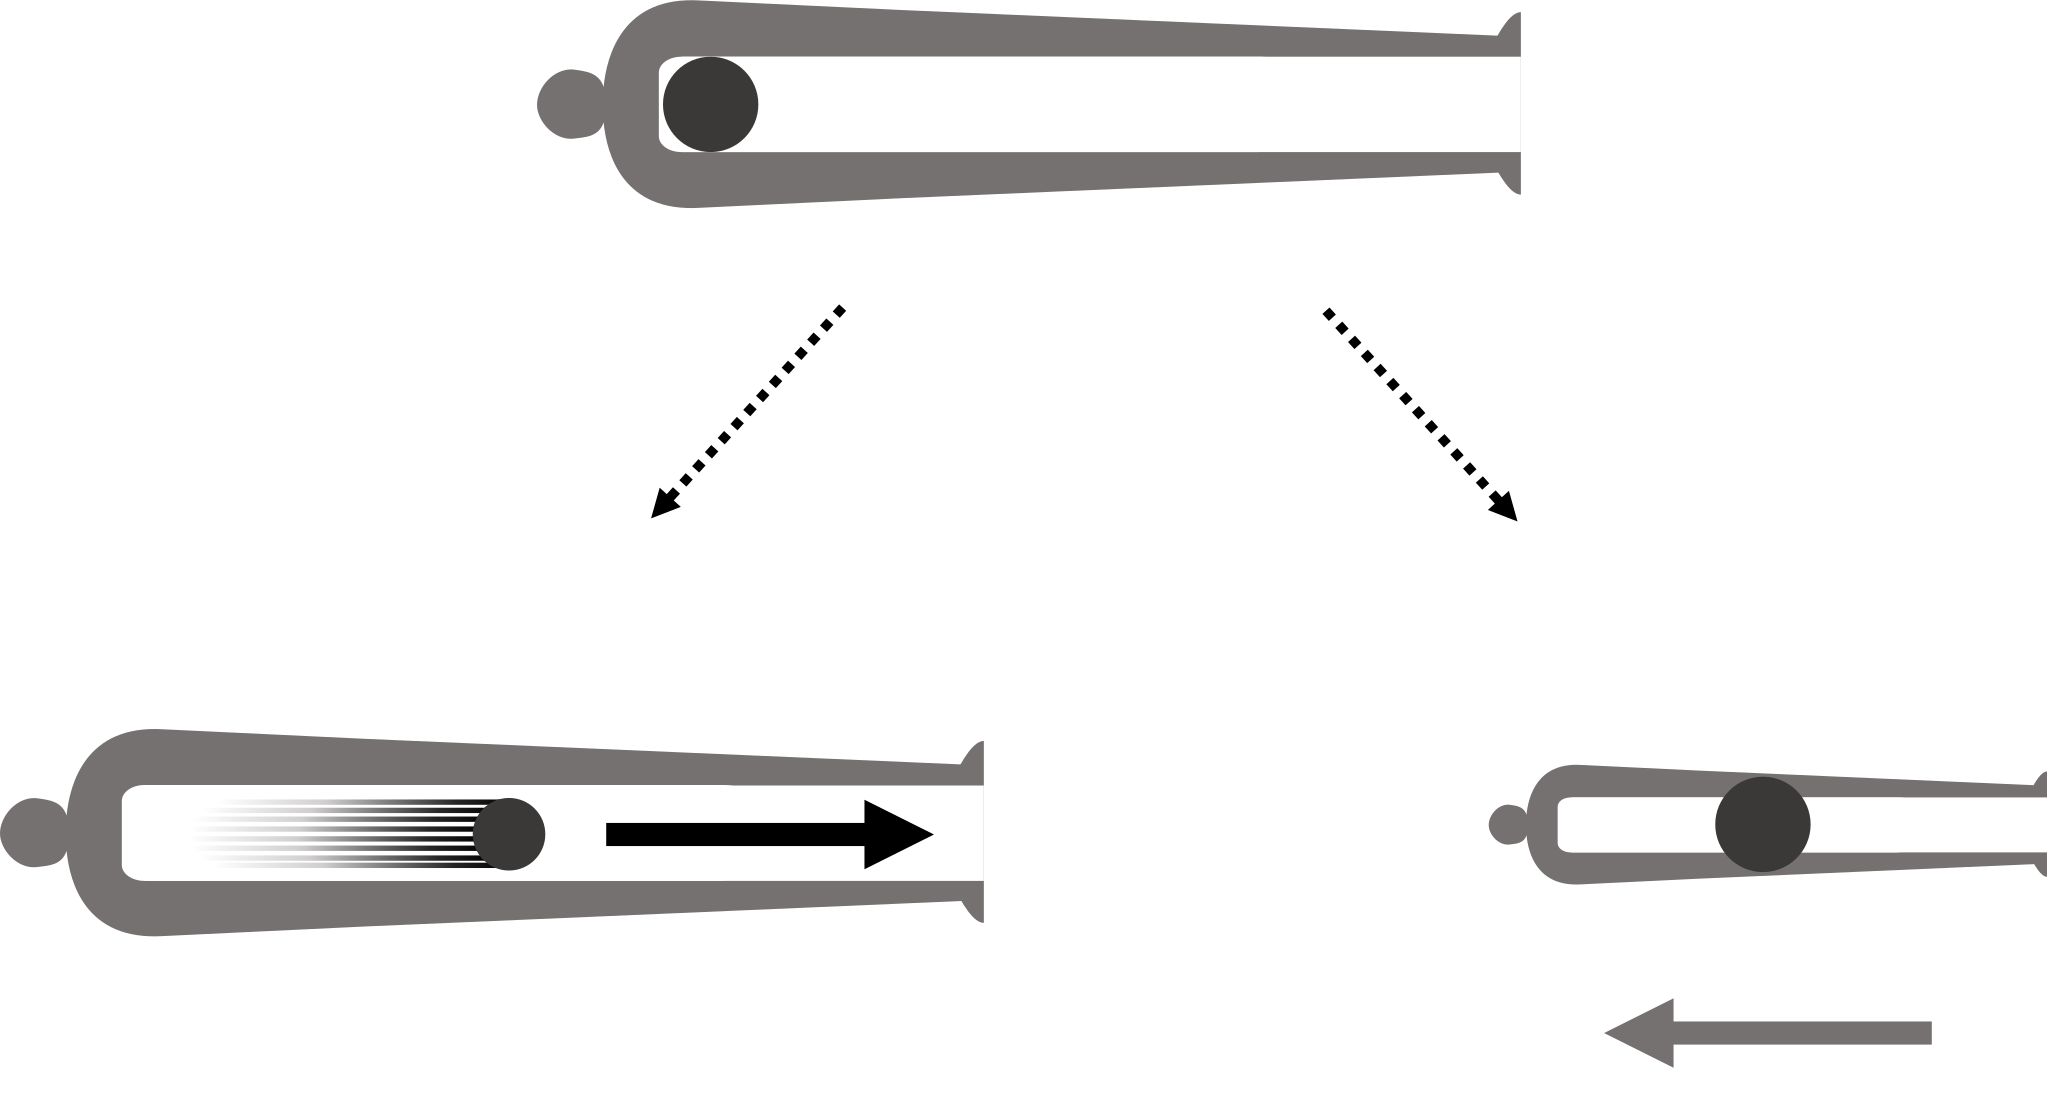
\includegraphics[width=8cm]{images/pdf/Cannon_Balls.pdf}
	\caption{A diagram showing why there must not be a contraction in the perpendicular direction to the frame's relative motion. The top Figure shows a ball and cannon at rest. The bottom figures show the cannon ball being fired in the frame of the cannon (left), where the moving ball has a contracted width, and (right) in the frame of the ball, where the canon is now moving and has a contract width, with the ball at rest being the same size. Both frames would contradict each other if there was a change in the width of moving objects, as the walls of the cannon and the surface of the ball would overlap in one frame and have a gap between them in the other. So, we require no size change perpendicular to the object's movement.}
	\label{fig: width contraction}
\end{figure}
%███████████

%Suppose we have a ball at rest in a pipe such that the ball touches the inner circumference of the pipe; if we were to make now the ball move, we would have it Lorentz contracted along the direction of the movement, but if we also had it contract perpendicular to the direction of movement then in the rest frame of the pipe we would have the ball smaller such that it no longer was touching the inner pipe, but if we changed to the frame of the ball it would be the pipe that was moving. We would expect the pipe to contract and be smaller than the ball (so that the ball would get stuck), so in the two different frames, we would have two contradictory outcomes. Still, we should be able to go from one frame to the other and not have these contradictions, so we require that there is no size change perpendicular to the object's movement.

From this paradox, we are only left with the possibility that the perceived travel time of the light must be longer in the track's \hyperlink{def-Reference-frame}{reference frame}, Meaning the light clock ticks slower to the \hyperlink{def-observer}{observer} on the track watching it as it moves.

How much slower the time is passing in the moving train relative to the track observer can be solved using the ratio of the lengths of the paths in each frame as shown in Figure (\ref{fig: train clock}), as this is the same ratio as the time between the ticks.

%█████████████
\begin{figure}[H]
	\figuretitle{Light Clock on a train}
	\centering
	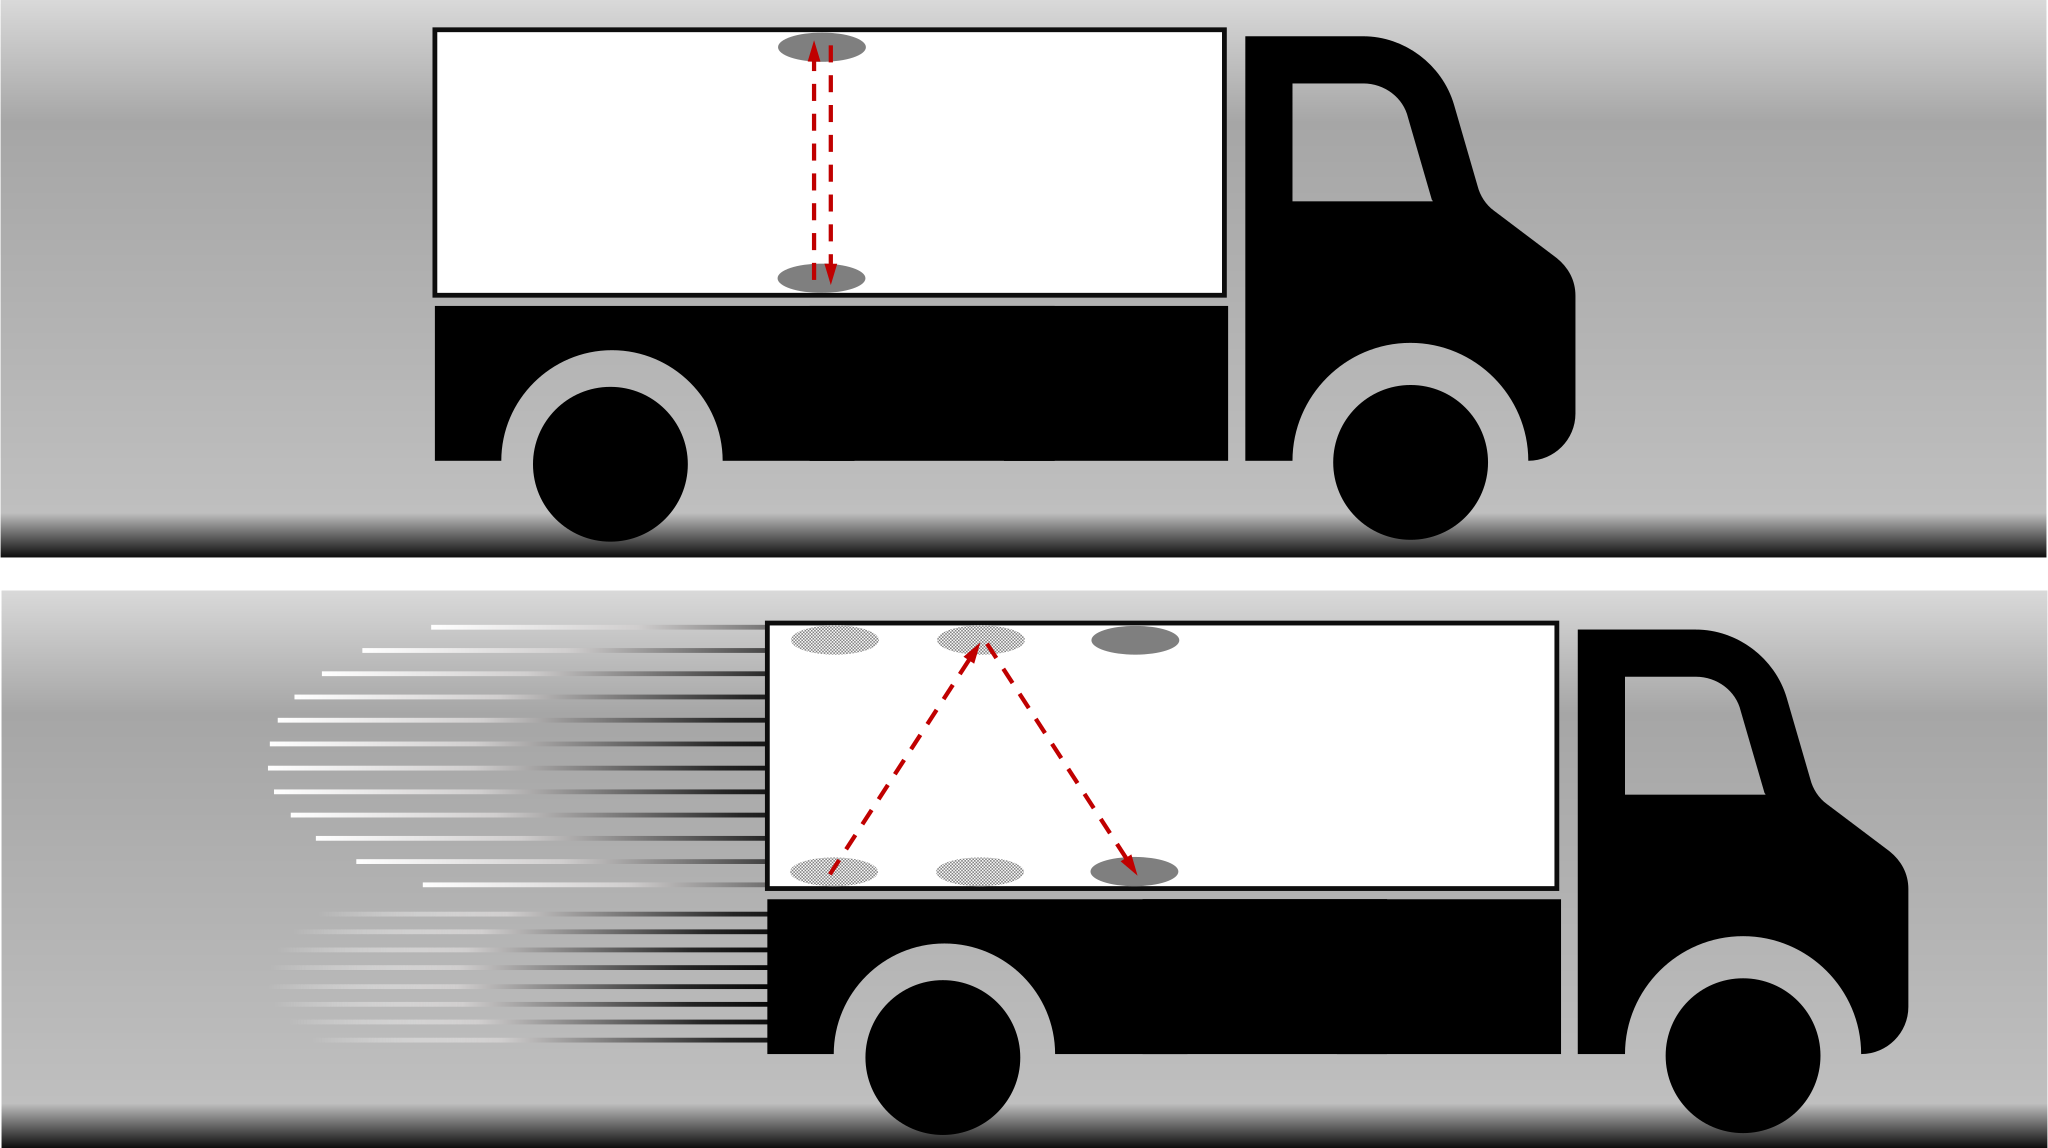
\includegraphics[width=8cm]{images/pdf/lorry_clock.pdf}
	\caption{A diagram, showing the extra distance light travels in the track's frame with the train moving, leading to the train's time being perceived to move slower to an observer in the track's frame of reference.}
	\label{fig: train clock}
\end{figure}
%███████████

The ticking slows down the same way for any type of clock.
If you were to play a movie on the train, it would take a longer time for it to play through from start to finish for an observer watching it from the track's \hyperlink{def-Reference-frame}{reference frame}.
The actual time itself is being slowed down.

The closer the train goes to the speed of light, the more significant the difference in how fast the track frame's time flows relative to the train frame's time.
This can be seen as a longer horizontal stretch in the path taken for the light from the perspective of someone standing still on the track, with the time between each tick approaching infinity as the speed of the train approaches the speed of light.

If now, we instead had two trains moving at the same speed relative to the track but in opposite directions.
Each train would see its light moving vertically up and down while the other train's light moves diagonally.
Hence, each train perceives the other train's clock ticking slower.
An observer in the track's reference frame would see the trains move at the same speed and, hence, the passage of time between ticks as being the same for both trains.
This concept is confusing and difficult to visualize, but it will get easier with practice.
For now, though, we will continue building up the concepts of special relativity.

%███████████████████████████████████████████████████████████████████
\subsection{Simultaneity}

Let us imagine a train in its \hyperlink{def-proper-frame}{rest frame}, with a light bulb in the middle and mirrors on the front and back walls.
Suppose the light bulb gives off a pulse of light.
The light will travel from the center of the train to the mirrors \hyperlink{def-simultaneity}{simultaneously} and back to the light bulb also \hyperlink{def-simultaneity}{simultaneously}.
But an \hyperlink{def-observer}{observer} on the track watching the train drive past will see the light bulb \hyperlink{def-simultaneity}{simultaneously} emit light in both directions and \hyperlink{def-simultaneity}{simultaneously} return to the bulb again.
However, the light reflects off each wall's mirrors at different times in the track's frame to do this, as shown in Figure (\ref{fig: train simultaneity}).
This is because the speed of light is the same for both directions, but the train is moving, meaning the back of the train is moving towards where the bulb was when the light pulse was emitted, making the distance traveled shorter.
The light travels a longer distance to the front wall due to the wall moving away from where it was emitted.
Because of this, the \hyperlink{def-observer}{observer} on the track will see the light hit the mirrors at different times.

%█████████████
\begin{figure}[htbp]
	\figuretitle{Simultaneity of Events in Different Frames}
	\centering
	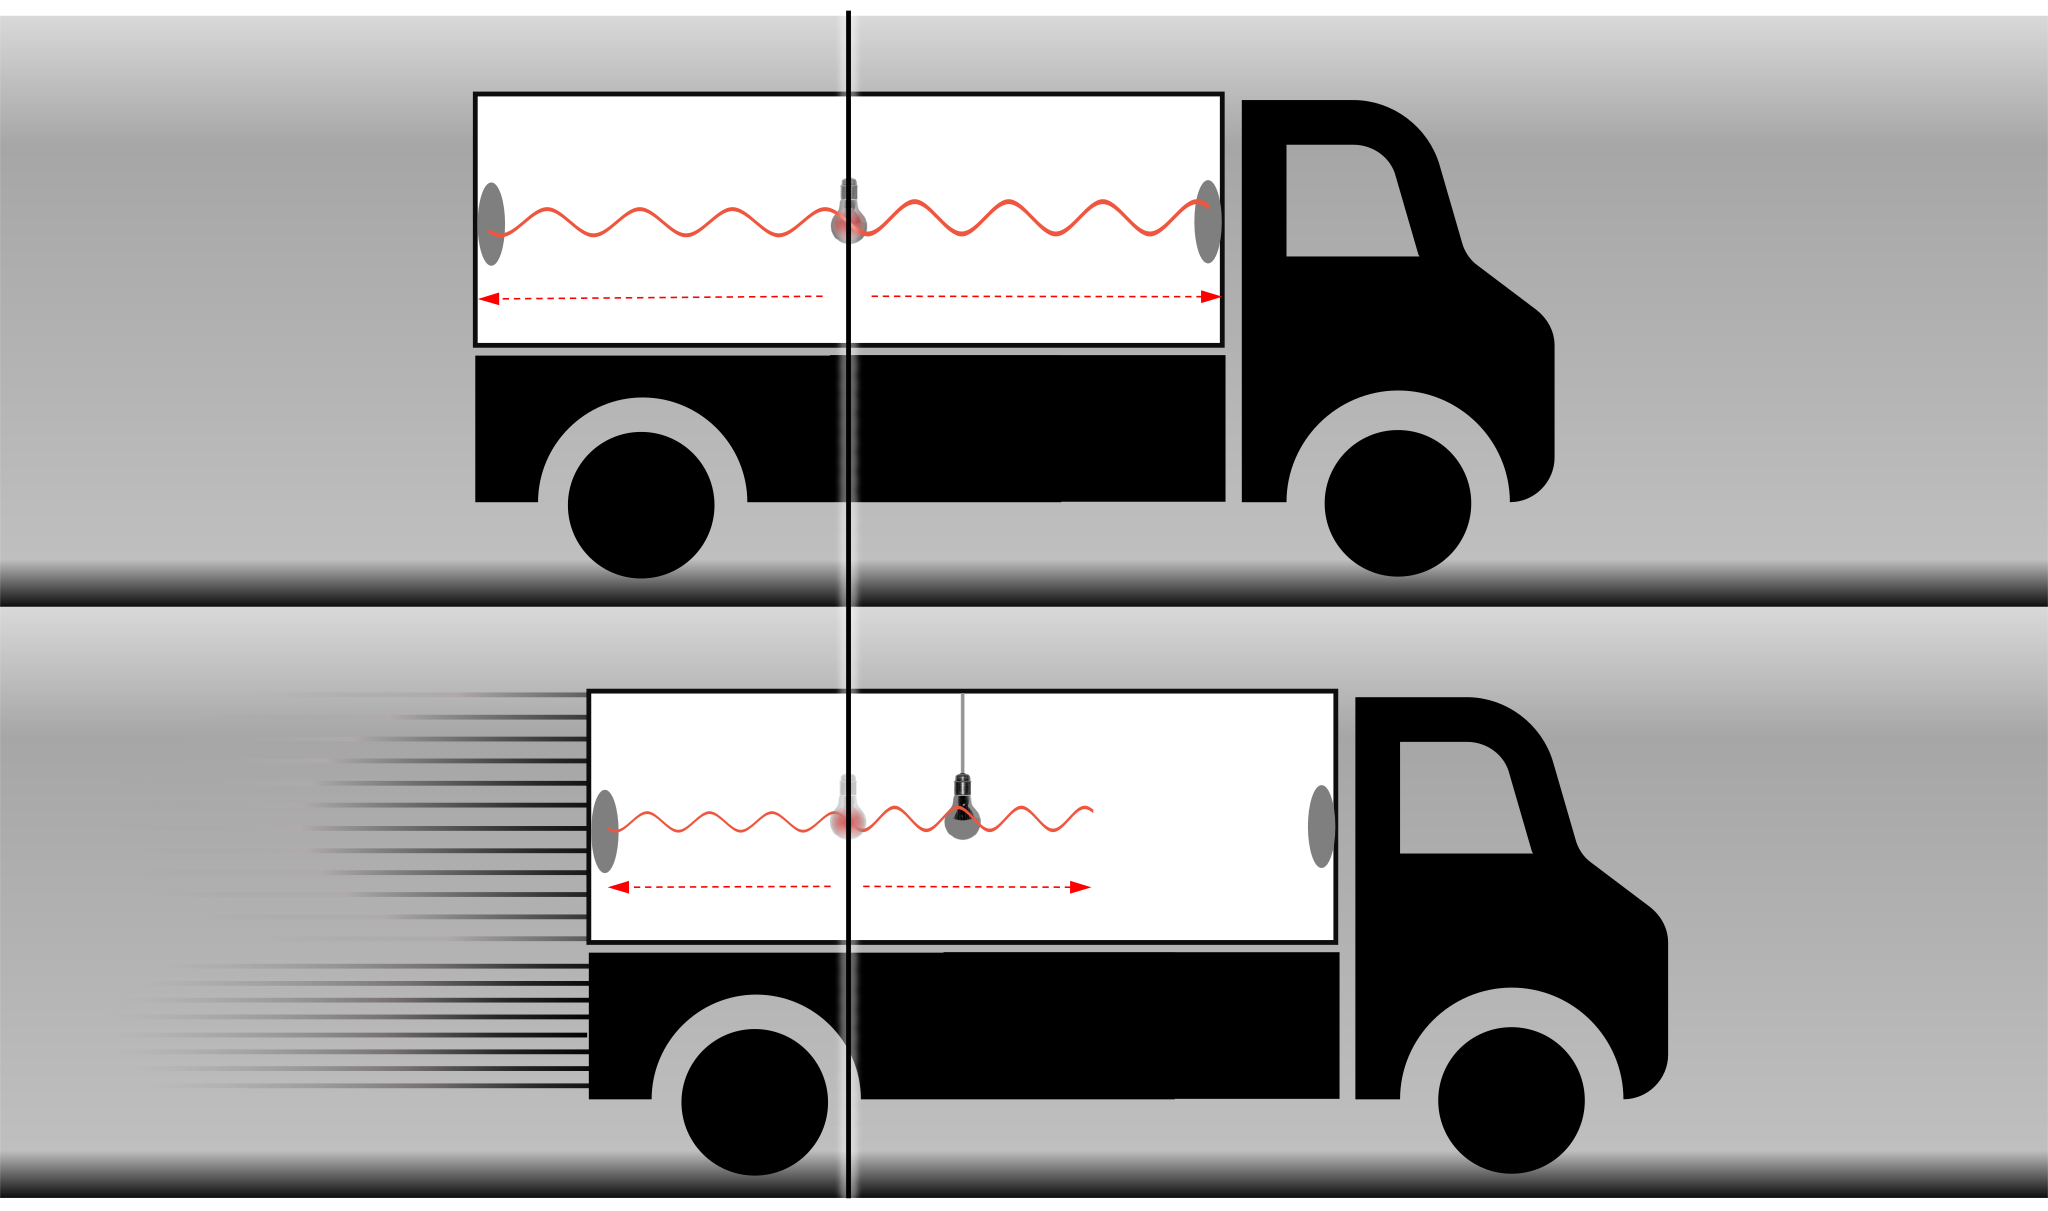
\includegraphics[width=8cm]{images/pdf/lorry_simul.pdf}
	\caption{A diagram showing how two \protect\hyperlink{def-event}{event}s of light reaching the two walls of the train are \protect\hyperlink{def-simultaneity}{simultaneous} in one frame but happening at different times in another, due to train's movement in the second frame and the speed of light remaining the same.}
	\label{fig: train simultaneity}
\end{figure}
%███████████

So, times of \hyperlink{def-event}{event}s (like when the light reaches either mirror) are different for \hyperlink{def-observer}{observer}s in different \hyperlink{def-Reference-frame}{reference frame}s, there is no one true order of \hyperlink{def-event}{event}s.
For example, an \hyperlink{def-observer}{observer} in a faster-moving train moving in an opposite direction would see the light reach the front wall first.
However, for all \hyperlink{def-observer}{observer}s, the light will return to the central light bulb \hyperlink{def-simultaneity}{simultaneously}.
If two \hyperlink{def-event}{event}s happen in the same position \hyperlink{def-simultaneity}{simultaneously}, then this happens \hyperlink{def-simultaneity}{simultaneously} in all frames of reference.
This means the light returns to the center of the light bulb \hyperlink{def-simultaneity}{simultaneously} in each frame.

A note here is that we are talking about when the events \textbf{actually} happen in each frame and not when the light from these events reaches the observer, which is later due to the time it takes the light to travel to the observer.
Also, I have left out any mention of \hyperlink{def-length-contraction}{length contraction} of the truck, which will be introduced in the next section, and why it needs to be equal in both directions from the lightbulb for the light to \hyperlink{def-simultaneity}{simultaneously} return to the light bulb.

%███████████████████████████████████████████████████████████████████
\subsection{Length Contraction}\label{sect: Length Contraction}

Suppose we have a train in its \hyperlink{def-proper-frame}{rest frame} with a square container with light emitted in all four directions from the center so that it will bounce off the mirrored sides of the train and return to the center \hyperlink{def-simultaneity}{simultaneously}.
We require that in the moving frame, they also all return to the center \hyperlink{def-simultaneity}{simultaneously}, as multiple \hyperlink{def-event}{event}s that happen at a single point \hyperlink{def-simultaneity}{simultaneously} in one frame, must happen \hyperlink{def-simultaneity}{simultaneously} in all other frames.
This time between the light being emitted and absorbed will be the \hyperlink{def-time-dilation}{dilated time}, that was described in section (\ref{Subsect: Time Dilation}).

To achieve this \hyperlink{def-simultaneity}{simultaneity} in the return of the light to the bulb, the total length of the path of light in each of the four directions must be the same.
As its speed is the same in all directions.
We can work out the length of the upward path from the \hyperlink{def-time-dilation}{time dilation} section (\ref{Subsect: Time Dilation}), and this is the length the path needs to be in the horizontal directions as well, the paths can only have this length if the train's length is contracted when moving, the exact amount of contraction can be worked geometrically, and it turns out that the ratio of the increase in the amount of time that passes before the light is reabsorbed is inversely proportional to the amount the train is contracted in the direction of its movement.

%█████████████
\begin{figure}[H]
	\figuretitle{Length Contraction of Moving Train}
	\centering
	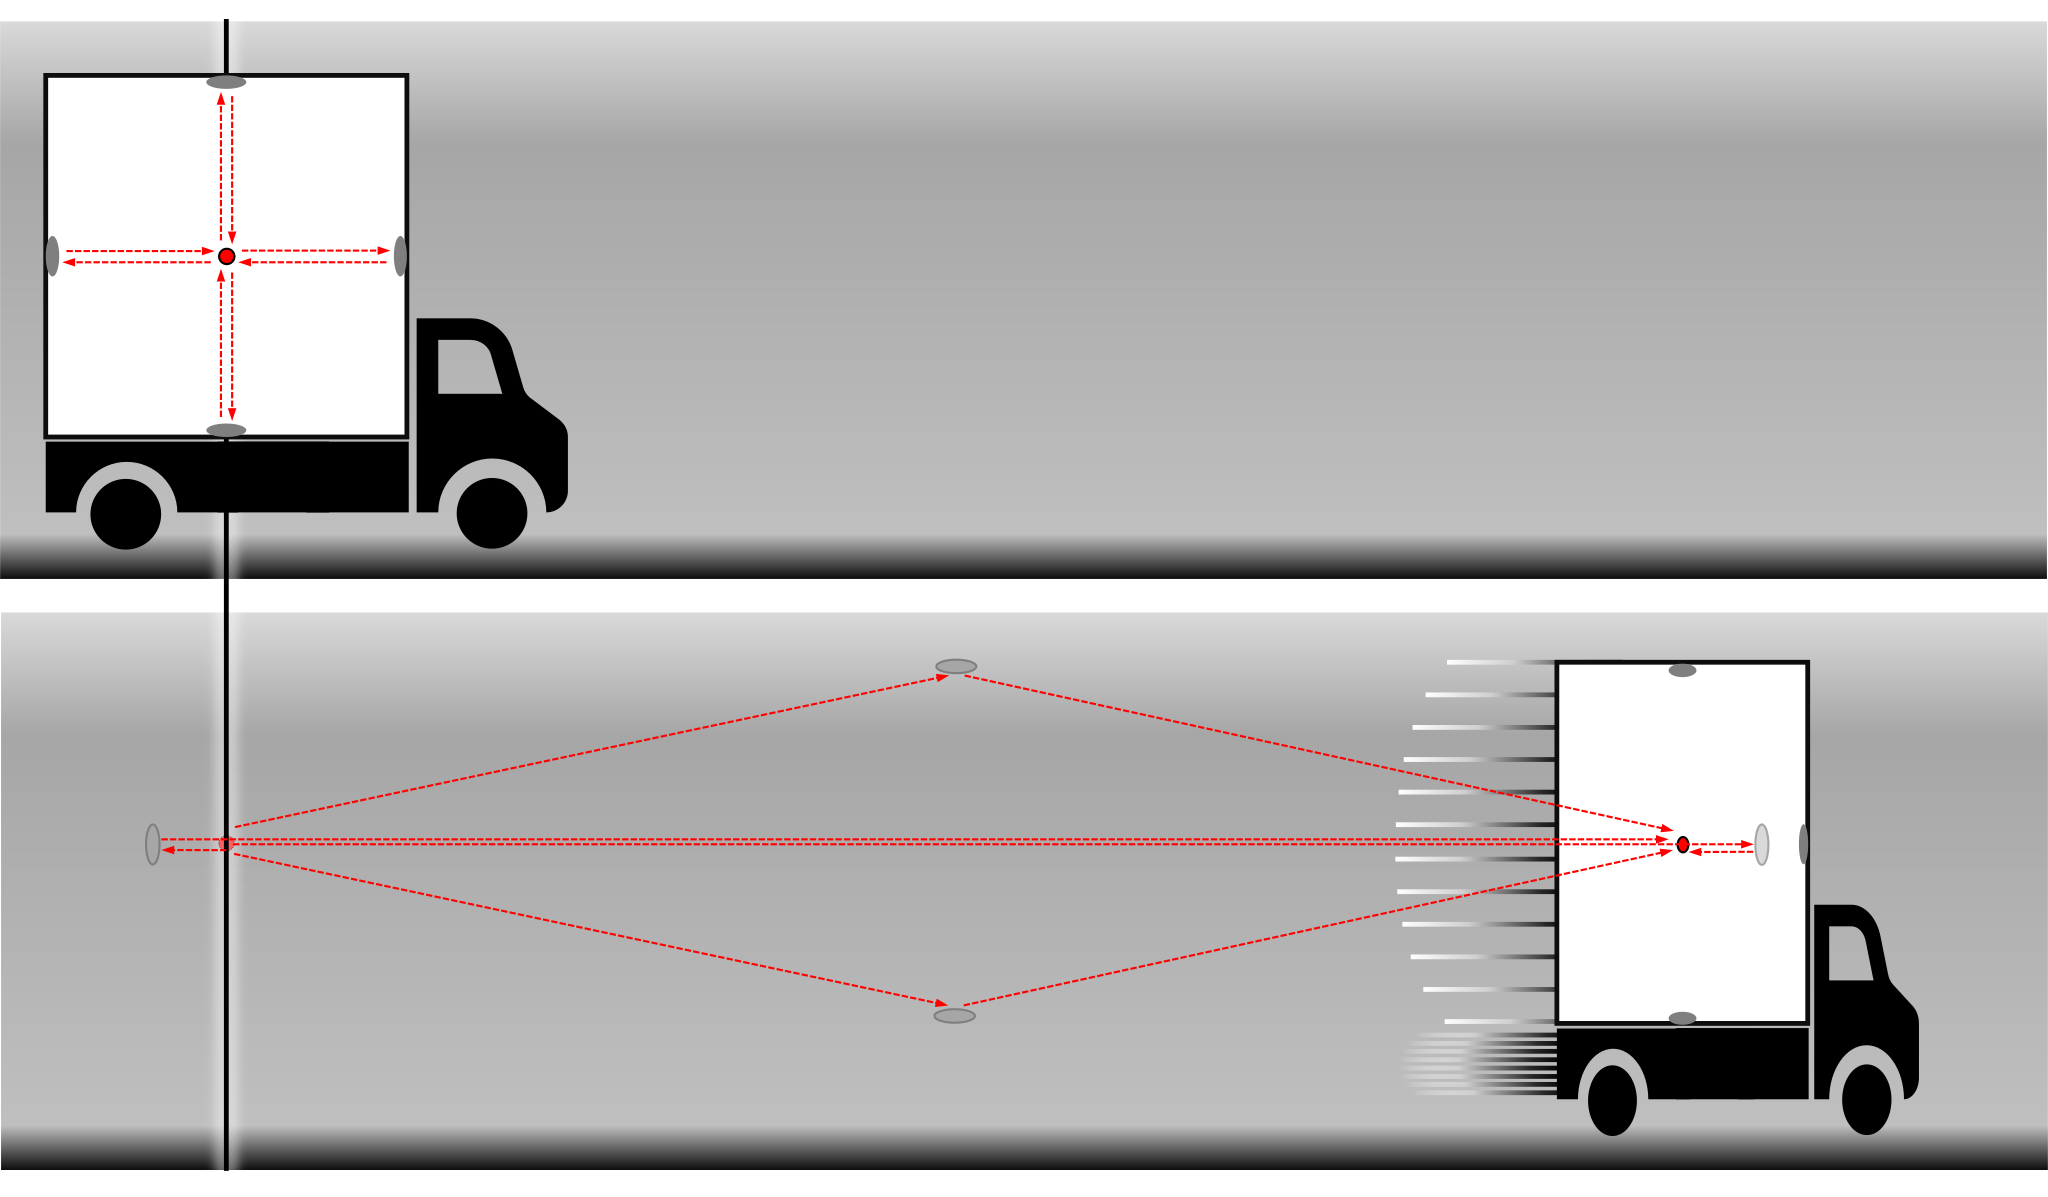
\includegraphics[width=8cm]{images/pdf/Full_Lorry_Transform.pdf}
	\caption{A diagram, showing a train with a square container in its \protect\hyperlink{def-proper-frame}{rest frame} (top), emitting light from a central bulb in the four directions, with all light being reflected by the mirrored sides back to the center. In the second frame with the train now moving (bottom), we see the train's length contracted and what the light paths would be in this frame.}
	\label{fig: full train transform}
\end{figure}
%███████████

So now we know that moving objects must shrink in the direction they move to allow for a consistent speed of light in each frame.
But this is not noticeable when objects move much slower than light speed.
If you are unsatisfied with this, the next section will reason the need for length contraction in another way.

% The faster you go, the closer things are in that frame, so it would take a shorter amount of time to get to places the closer you get to the speed of light (is this true)

%██████████████████████
\subsubsection{Another Illustration of Length Contraction}

Suppose we have three equally distanced cars at rest on the road, as shown in Figure (\ref{fig: cars}).
If the middle car sends out a pulse of light, it will reach the front and back car at the same time for the road \hyperlink{def-observer}{observer} and the \hyperlink{def-observer}{observer}s in the car. When it reaches them both, all the cars accelerate for a predetermined fixed amount of time.
This means that after this acceleration period, the cars are now moving but still equally spaced relative to the \hyperlink{def-observer}{observer}s in the cars and the \hyperlink{def-observer}{observer} on the road.
As for all \hyperlink{def-observer}{observer}s, the light reached the front and back cars at the same time.

Now, suppose we do this a second time, with the middle car releasing another pulse.
In that case, we have in the frame of the \hyperlink{def-observer}{observer}s in the cars: again, with the front and back drivers receiving the pulses simultaneously, meaning that they will start accelerating simultaneously.
After the acceleration has finished, the distances between the cars will be the same for the car observers.
But for the road \hyperlink{def-observer}{observer}, they see the back car receive the signal first, as that car is moving towards the point where the light pulse was emitted, and the front car is moving away from it.
This would mean the back car would start accelerating first to get to the final constant velocity and get closer to the front car before the front car begins to accelerate to that same final speed that the back car had already reached.
Hence, the cars end up closer together after all this.
The \hyperlink{def-observer}{observer}s in the car and the road \hyperlink{def-observer}{observer} disagree with what the distances between the cars are.
This contraction of length between cars, in the road's frame in which the cars are moving, is called Lorentz \hyperlink{def-length-contraction}{length contraction}, which means that objects that are moving faster become shorter, and the distances between the objects also become shorter.

%█████████████
\begin{figure}[H]
	\figuretitle{Length Contraction Between Three Accelerating Cars}
	\centering
	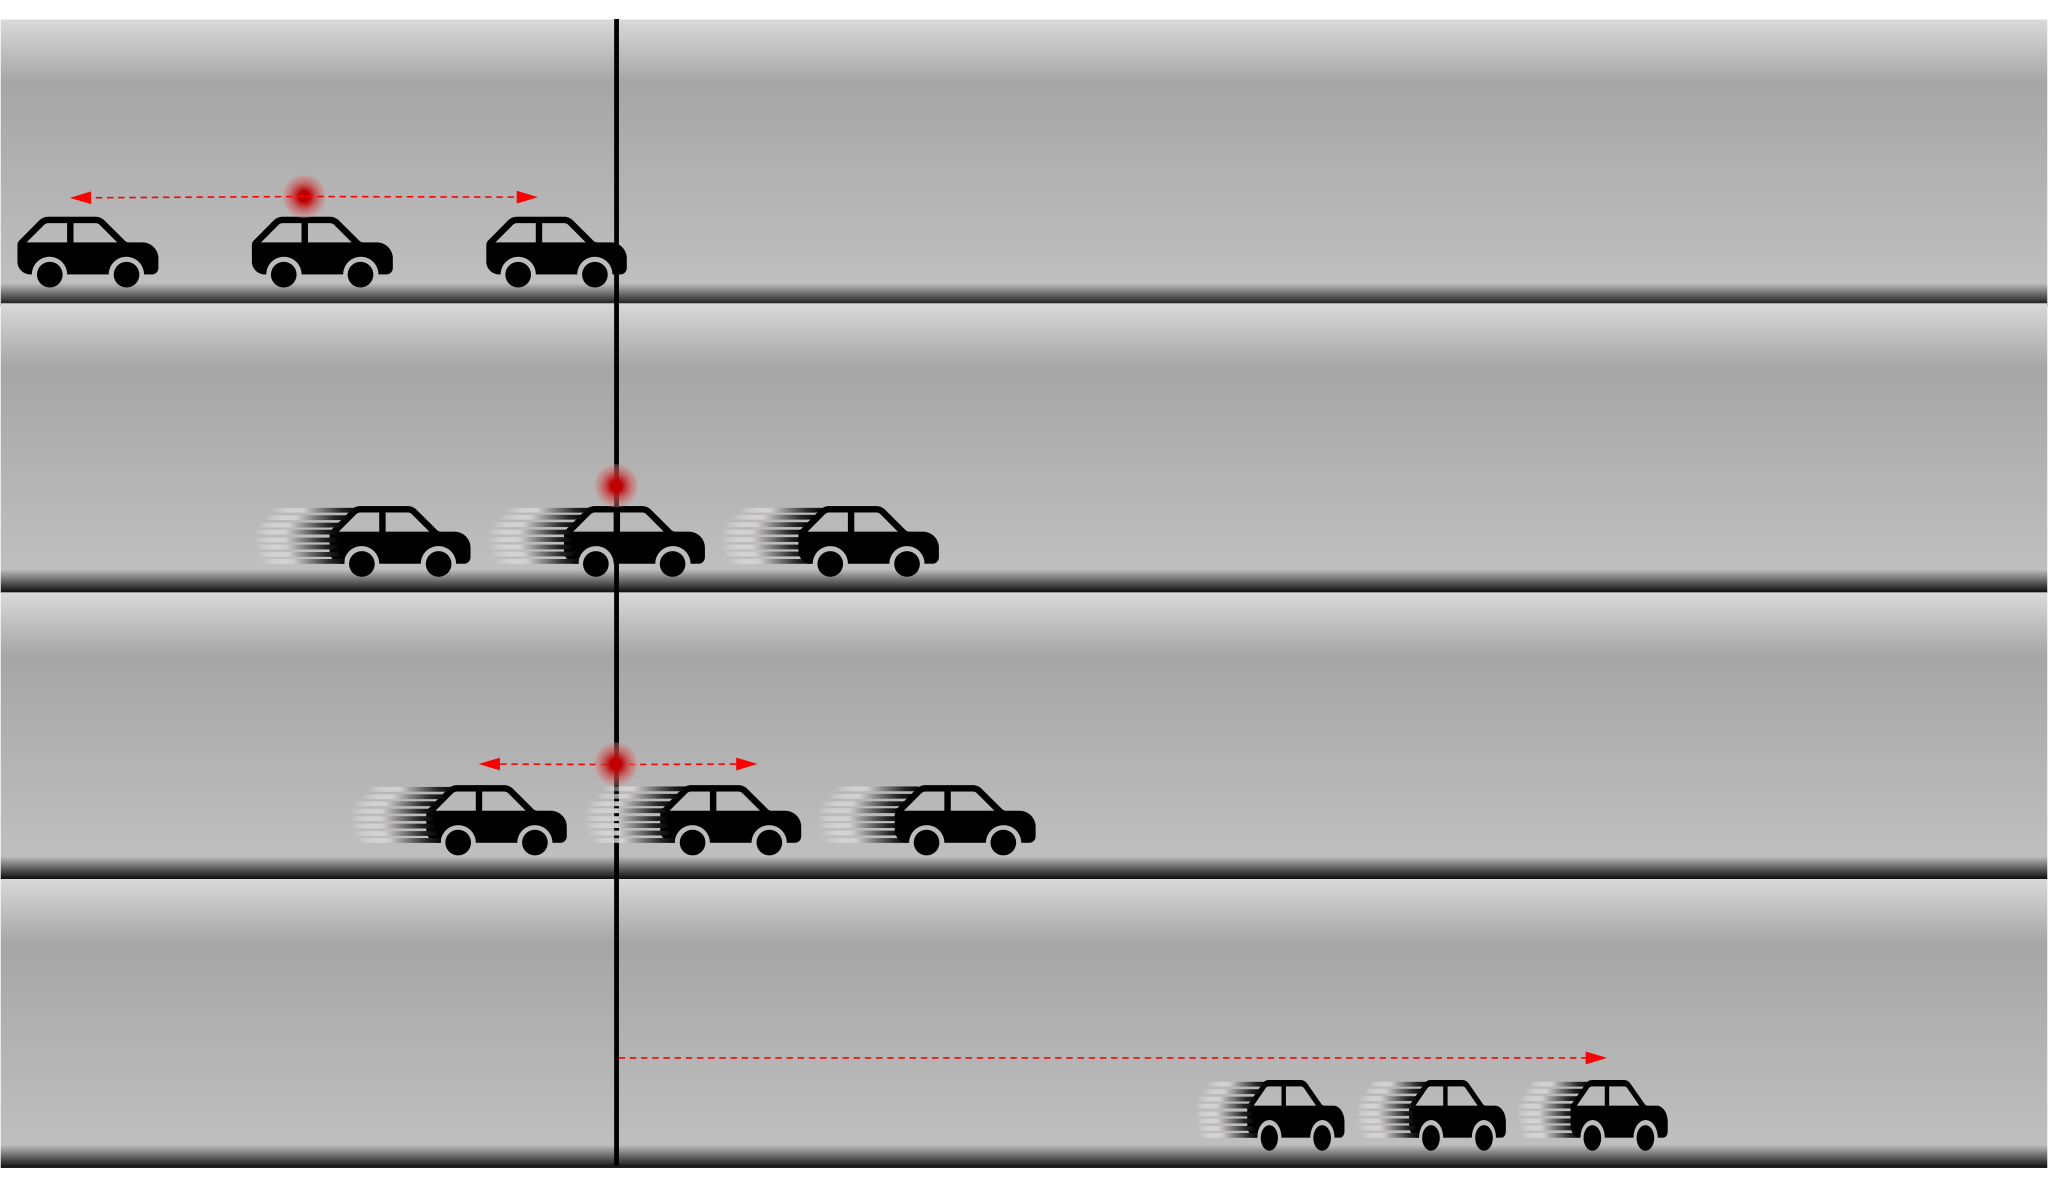
\includegraphics[width=8cm]{images/pdf/cars.pdf}
	\caption{A diagram, illustrating an experiment with three cars initially at rest and equally spaced on a road. The middle car emits light that reaches the front and back cars \protect\hyperlink{def-simultaneity}{simultaneously}, triggering all cars to accelerate for a predetermined time. Now another light is emitted from the middle car after the acceleration has finished, the road \protect\hyperlink{def-observer}{observer} sees this second light pulse reach the back car first, as it is moving towards where the light had been emitted, this causes it to begin accelerating before the front car. This results in the cars being closer together after acceleration, demonstrating Lorentz \protect\hyperlink{def-length-contraction}{length contraction}. However, to the car \protect\hyperlink{def-observer}{observer}, the distance between the cars remains unchanged from the initial distances.}
	\label{fig: cars}
\end{figure}
%███████████

%███████████████████████████████████████████████████████████████████
%███████████████████████████████████████████████████████████████████
\section{Doppler Effect}

*** start

If we have a source at rest, emitting circular pulses of light with equal times between each pulse, we will have concentric circular pulses in this frame, but if we move to a frame where the source is now moving to the right, each circular pulse is now being emitted from a different position as the source is moving.
Due to the source moving, each pulse will be emitted closer to the right-hand side of the previous pulses, creating a bunching up of the pulses (increase in frequency) in the direction of movement and a spreading out (decrease in frequency) of the pulses in the opposite direction.
This also happens in the classical version of the \hyperlink{def-doppler-effect}{Doppler effect}.
For example, you will notice that an ambulance or police car sounds different when driving toward or away from you due to the bunching up and spreading out of the sound waves in the direction and opposite of the moving vehicle.
In special relativity, we also must take the \hyperlink{def-time-dilation}{time dilation} of the pulses into account, as there will be a longer time between each subsequential pulse.
This is Due to objects moving relative to an observer having their perceived time moving more slowly.
This has a decreasing effect on the frequency in all directions.
However, directly in the direction of movement of the source, this is outweighed by the frequency increase from the previous bunching-up effect.
Since the energy of the light is proportional to the frequency, it is also increased in the direction of motion of the source due to the \hyperlink{def-doppler-effect}{Doppler effect}s and decreased in the opposite direction.

%█████████████
\begin{figure}[H]
	\figuretitle{Spherical Waves From a Moving Source}
	\centering
	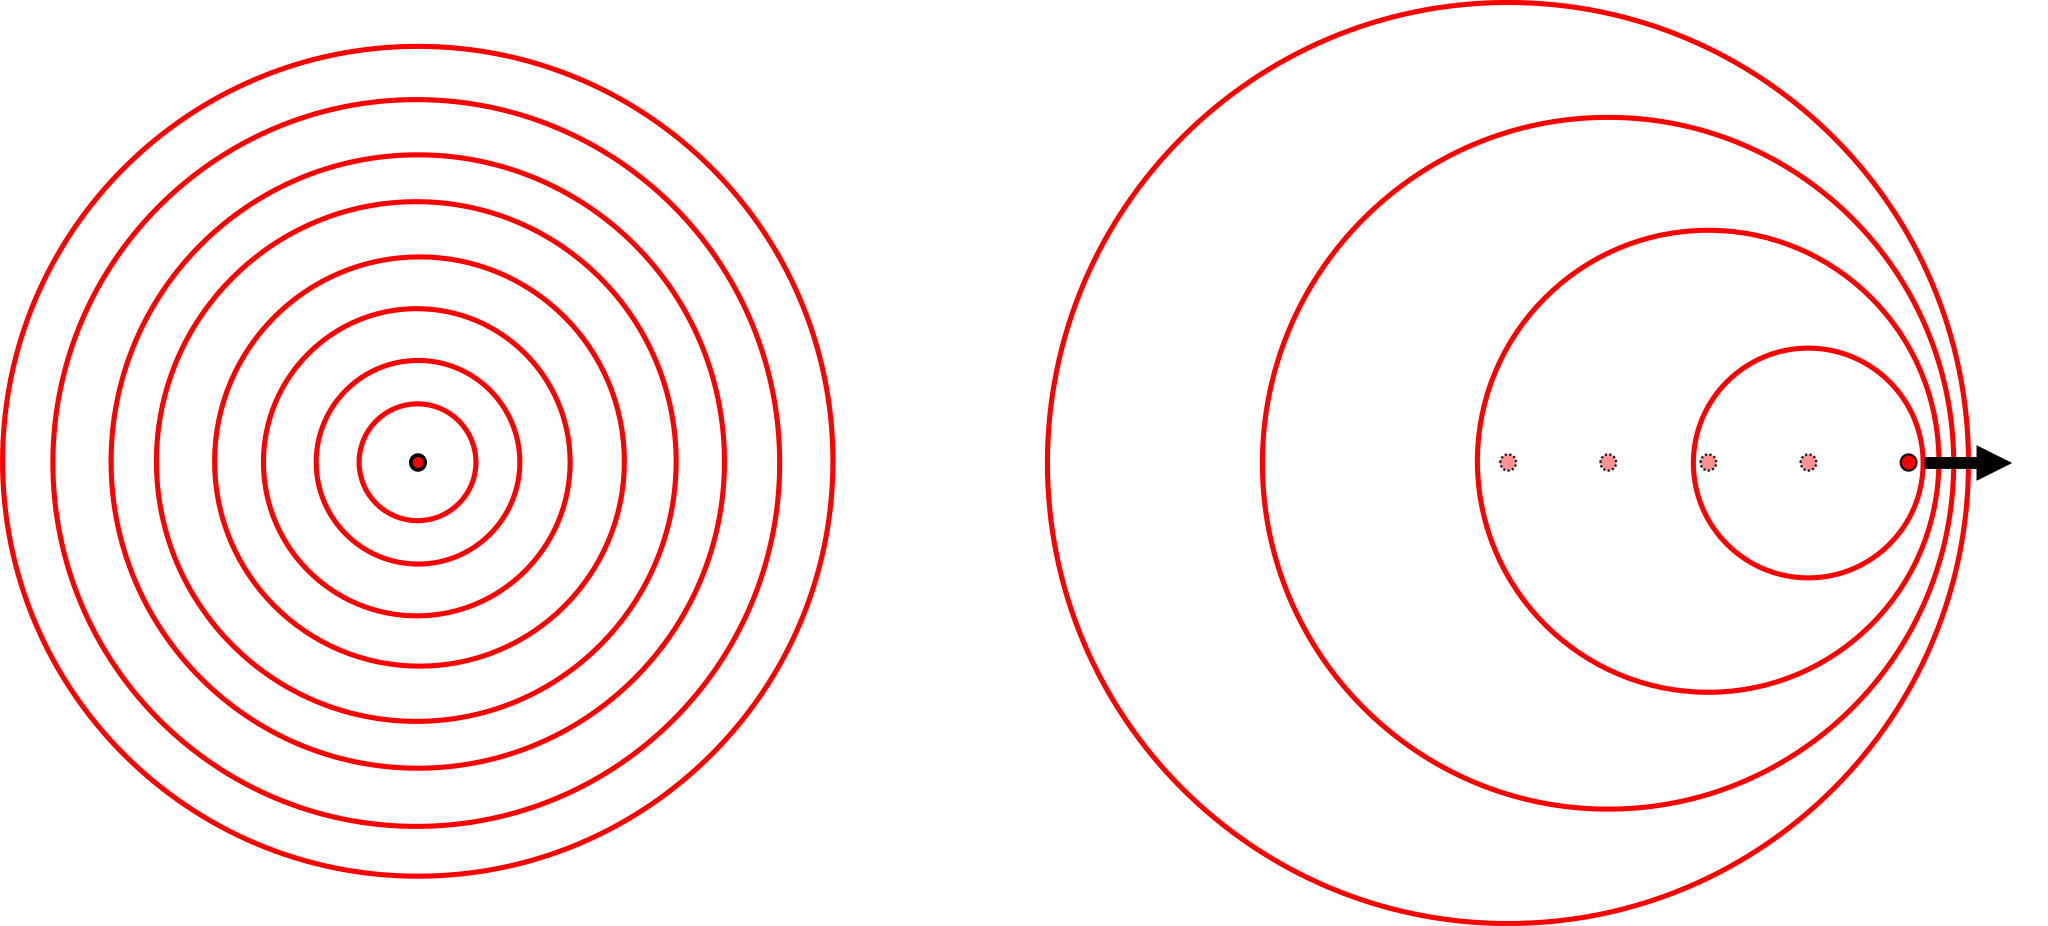
\includegraphics[width=8cm]{images/pdf/Doppler.pdf}
	\caption{A diagram showing (left) a central source at rest emitting several circular pulses of light with equal time between each pulse, (right) the same source in a frame where it is now moving and emitting circular pulses of light, but each subsequential pulse is emitted from a different position as the source is moving, marked by a faded dot.}
	\label{fig: doppler effect intro}
\end{figure}
%███████████

One thing not mentioned yet in this picture so far is how the light is also affected by what is called the \hyperlink{def-aberration}{aberration}, which is the change in the angular distribution of the light at each part of the spherical pulses, which will be explained in the next section.

%███████████████████████████████████████████████████████████████████
%███████████████████████████████████████████████████████████████████
\section{Aberration}

Here, we will talk about what the \hyperlink{def-doppler-effect}{Doppler effect} in the previous section has yet to show, which is the effect on the angular distribution of the light in each part of the spherical pulses.
We will show that there is a higher concentration of light in the direction of the source's movement, as shown in Figure (\ref{fig: train aberrated}).

With the help of the \hyperlink{def-length-contraction}{length contraction} section (\ref{sect: Length Contraction}), let us imagine a train with a spherical mirrored container, a central bulb emits light in all directions, in the \hyperlink{def-proper-frame}{rest frame} all light reaches the spherical wall at the same time and returns to the center bulb \hyperlink{def-simultaneity}{simultaneously} aswell.
Then in the moving frame, we have the spherical container \hyperlink{def-length-contraction}{length contracted} and the light moving at the same speed but reflecting off the walls at different times, returning to the center bulb simultaneously, for this to be true, the directions of the light have to be aberrated (have their direction of propagation changed) in the way shown in the diagram to allow for this \hyperlink{def-simultaneity}{simultaneous} return to the bulb.

%█████████████
\begin{figure}[htbp]
	\figuretitle{Aberration of Light on a train}
	\centering
	\begin{subfigure}{.49\textwidth}
		\centering
		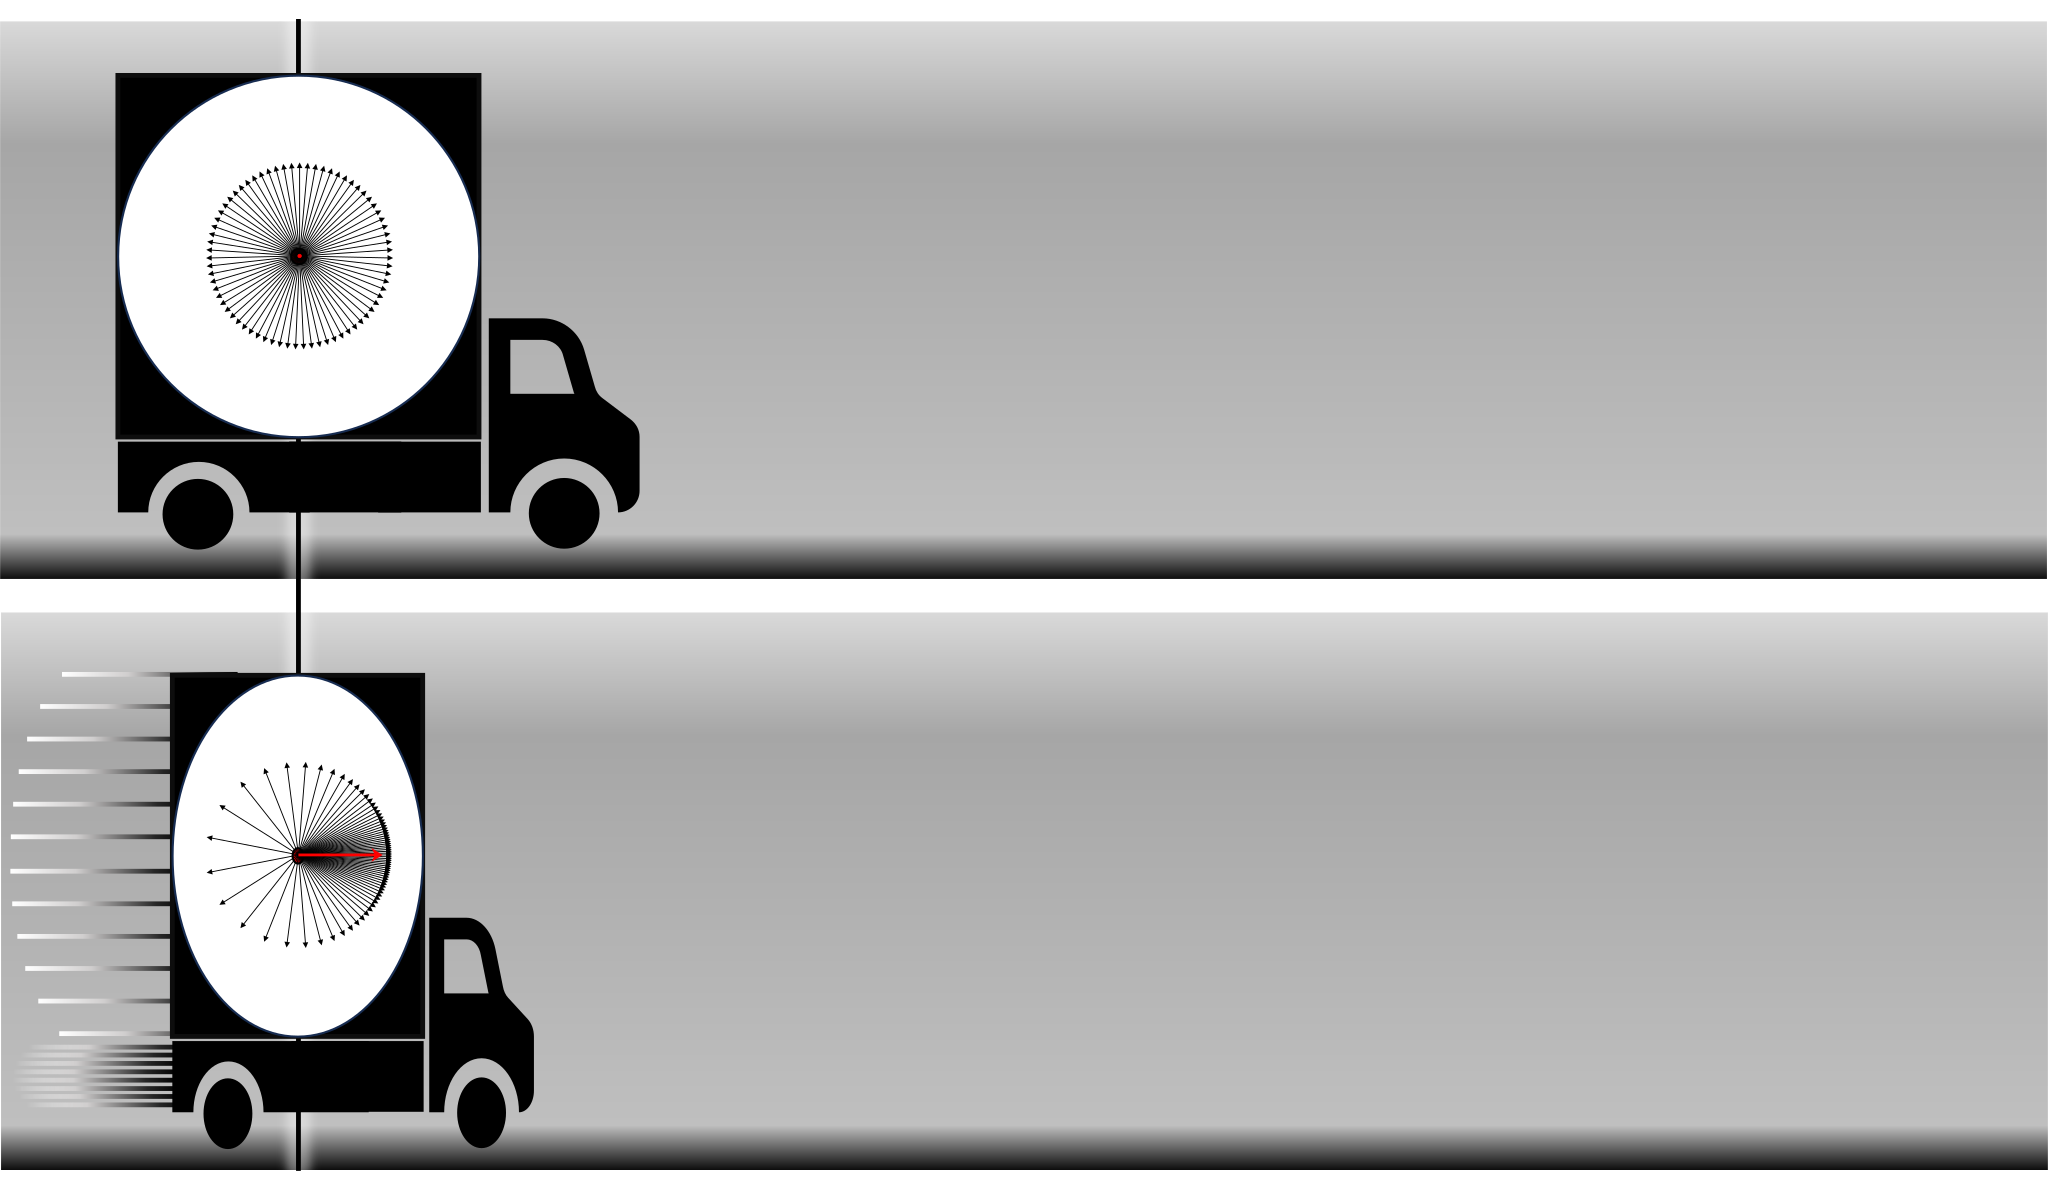
\includegraphics[width=5.5cm]{images/pdf/Aberrated_lorrys_1.pdf}
		\caption{Pulse emitted}
		\label{fig: train aberrated 1}
	\end{subfigure}
	\begin{subfigure}{.49\textwidth}
		\centering
		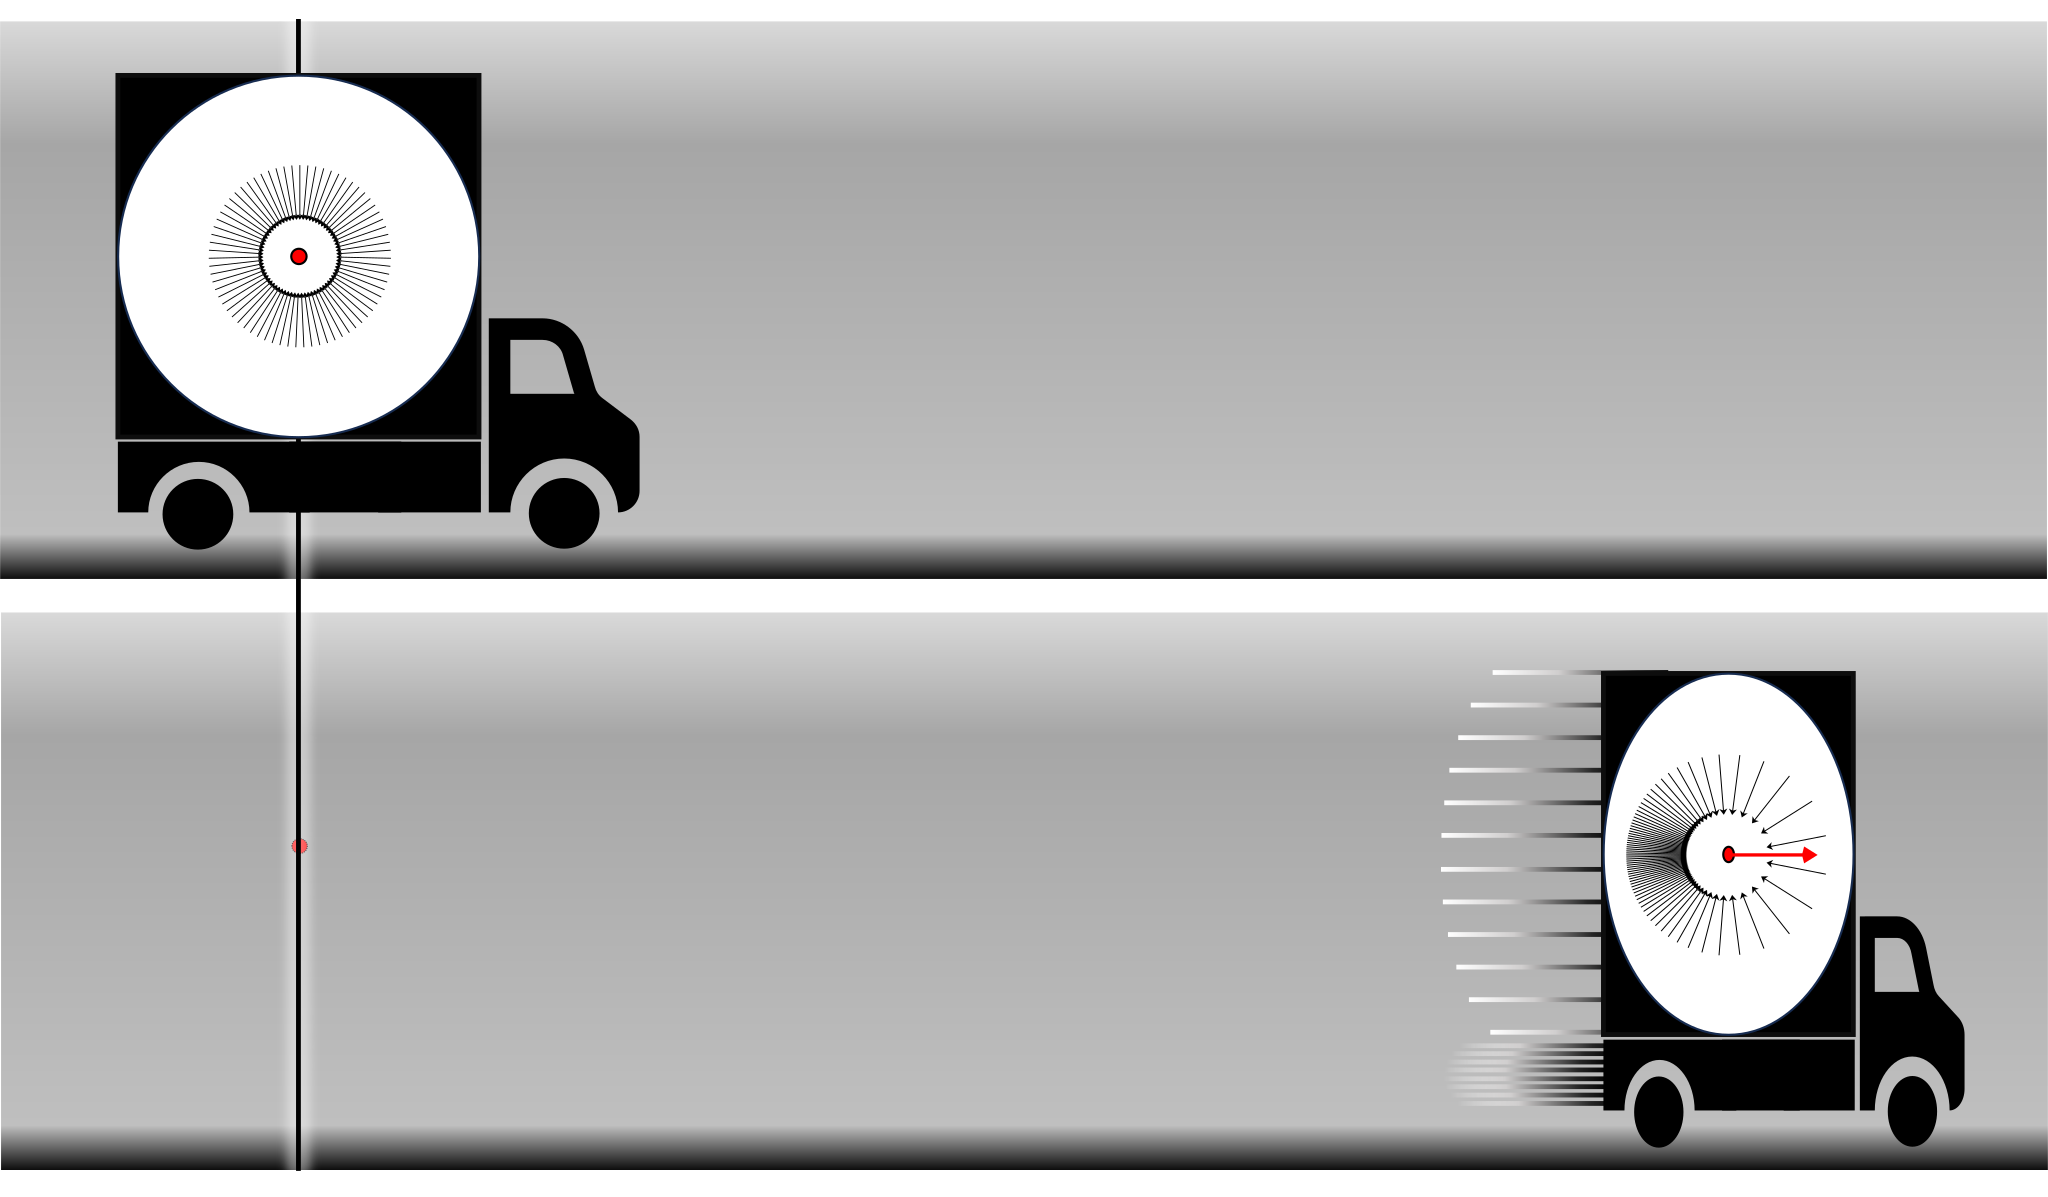
\includegraphics[width=5.5cm]{images/pdf/Aberrated_lorrys_2.pdf}
		\caption{Pulse absorbed}
		\label{fig: train aberrated 2}
	\end{subfigure}
	\caption{Two diagrams of a train with a spherical container in two different frames, a light pulse is emitted from the center of the container (left) and reflected back by the mirrored wall to be absorbed in the center again (right), the train in its \protect\hyperlink{def-proper-frame}{rest frame} (top of both figures) shows an evenly distributed outward light pulse, but in the frame, with the moving train (bottom of both figures) the emitted light is now more concentrated in the direction of the train's movement, which is required to allow the light to be reflected and returned to the center of the train \protect\hyperlink{def-simultaneity}{simultaneously}.}
	\label{fig: train aberrated}
\end{figure}
%███████████

%█████████████████████████████████████
\iffalse javascript{Aberration} \fi %█
%█████████████████████████████████████

From the diagrams, you can see how light is aberrated when emitted from a moving source relative to its \hyperlink{def-proper-frame}{rest frame} and when being absorbed by a source, the faster the source is moving, the more the direction of each part of the light pulse is aberrated.

% re-word next paragraph

If the speed of a source was to approach the speed of light, all emitted light's propagation direction would approach the direction of movement of the source.
If the source could theoretically reach the speed of light, all light would be emitted in the direction of the source but also move at the same speed.
That is, the source would move with the emitted light, and it would not leave the vicinity of the source.
The rate at which it emits the light would also tend to zero.
If a photon theoretically had mass and its influence of the gravitational force moved at the speed of light, then we would not be able to feel any gravitational effects from this theoretical photon with mass outside its vicinity.
This is due to all its gravitational field being propagated in the direction of its movement and at the same speed as the photon.

Another note is that in astrophysics, it must be taken into account that the Earth's view of the universe is distorted by \hyperlink{def-aberration}{aberration} when looking through telescopes, with the aberrational effect depending on where it is in its rotation around the sun.

We will look at the combination of the Doppler effect and aberration after a side note on velocity transforms for velocities less than that of light.

% as shown in diagram ref{...}. *** diagram of Earth's view of the universe is distorted from the \hyperlink{def-aberration}{aberration} (example on wiki) ***

%███████████████████████████████████████████████████████████████████
\subsection{General Velocity Transformation}

We looked at how velocities at the speed of light change between different frames of reference, that is, how their directions are aberrated.
However, for objects moving at speeds less than light, we need the transforming speeds to be different as well as aberrated due to the \hyperlink{def-transform}{transform} needing to tend towards the classical \hyperlink{def-transform}{transform} as the speeds tend towards zero.
To understand the general velocity \hyperlink{def-transform}{transformation}, some mathematical detail is needed, so we will need to brush over this for now.

%███████████████████████████████████████████████████████████████████
%███████████████████████████████████████████████████████████████████
\section{Relativistic Beaming}

When the Doppler effect and relativistic aberration are taken together, it is known as relativistic beaming.
If we have a source in its \hyperlink{def-proper-frame}{rest frame} emitting a spherical pulse of light with evenly distributed angles.
Then in a second frame with the source now moving, the emitted light will have from the Doppler effect, that this spherical pulse's wavelength is bunched up in the direction of movement (giving a change in the color of the light), with the aberrational effect giving the angular spread of the light at a higher concentration in the direction of the movement of the source, as shown in figures (\ref{fig: Relativistic Beaming}).

%█████████████
\begin{figure}[H]
	\figuretitle{Relativistic Beaming of Emitted Light}
	\begin{subfigure}{.49\textwidth}
		\centering
		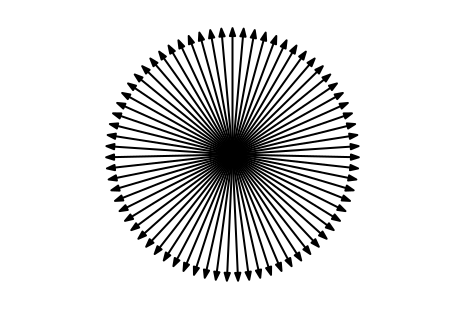
\includegraphics[width=5cm]{images/pdf/Rest_velocities.pdf}
		\caption{\hyperlink{def-proper-frame}{rest frame}}
	\end{subfigure}
	\begin{subfigure}{.49\textwidth}
		\centering
		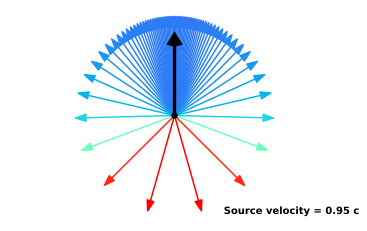
\includegraphics[width=5cm]{images/pdf/Aberrated_velocities.pdf}
		\caption{Moving frame}
	\end{subfigure}
	\caption{Outward light pulse from source in a rest and moving frame.}
	\label{fig: Relativistic Beaming}
\end{figure}
%███████████

%█████████████
\begin{figure}[H]
	\figuretitle{Relativistic Beaming Received Light}
	\begin{subfigure}{.49\textwidth}
		\centering
		\includegraphics[width=5cm]{images/pdf/Rest_velocities_inwards.pdf}
		\caption{\hyperlink{def-proper-frame}{rest frame}}
	\end{subfigure}
	\begin{subfigure}{.49\textwidth}
		\centering
		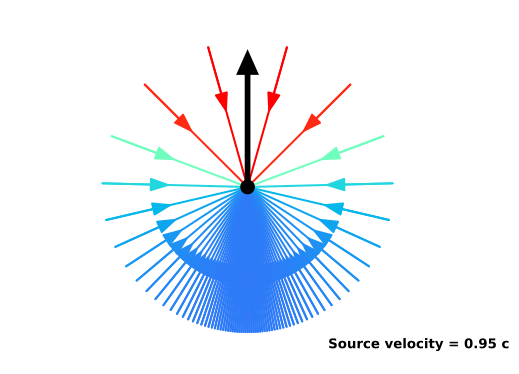
\includegraphics[width=5cm]{images/pdf/Aberrated_velocities_inwards.pdf}
		\caption{Moving frame}
	\end{subfigure}
	\caption{Inward light pulse from source in its rest and moving frame.}
	\label{fig: Relativistic Beaming Recieved}
\end{figure}
%███████████

For astrophysics, we need to consider this beaming when looking at distant stars that are moving relative to us so that we can accurately calculate their brightness and the spectrum of light that they are emitting, along with some other things.
We also need to consider that the position we are currently seeing the stars in is their past position due to the delay in light traveling to us on Earth, which is referred to as the retarded position.
We will talk about this next.

%███████████████████████████████████████████████████████████████████
\subsection{Retarded Field}

If a source in its rest frame continually emits pulses of light with a constant time between each pulse, we get what is shown in Figure (\ref{fig: multiple emitting pulses rest frame}).
If we wanted to know what this light field looked like in the source's moving frame, we would need to take into account that the source is moving so that the position the source emitted each pulse from is its past position (retarded position)and that we have the dilated time between pulses in this moving frame, so using this and the beaming effect from the previous section we get the light field as shown in Figure (\ref{fig: multiple emitting pulses moving frame}).
From this, we can work out the distribution and, hence, the concentration of the light for any moving source relative to that of it at rest.
If you look closely at the diagrams, you will see the aberrated rings of all the pulses, all with different points from which they were emitted, with them being more compact in the direction of the source's movement.

%█████████████
\begin{figure}[H]
	\figuretitle{Field of Light Pulses from a Source}
	\begin{subfigure}{.49\textwidth}
		\centering
		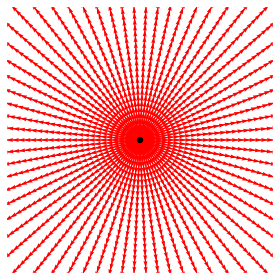
\includegraphics[width=5cm]{images/pdf/Field_Rest_Frame.pdf}
		\caption{Source's Rest Frame}
		\label{fig: multiple emitting pulses rest frame}
	\end{subfigure}
	\begin{subfigure}{.49\textwidth}
		\centering
		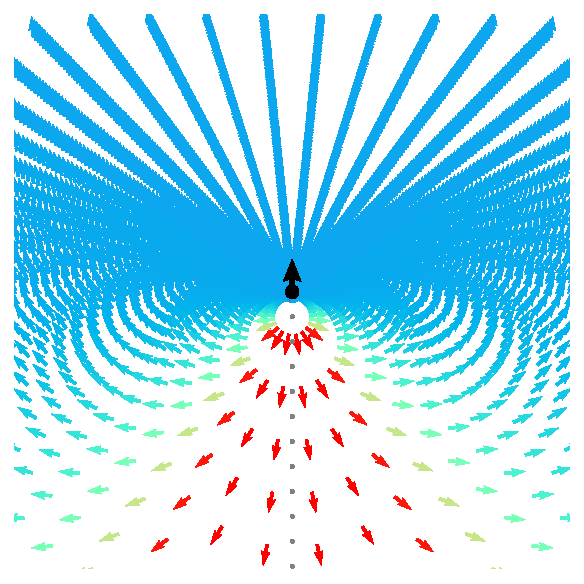
\includegraphics[width=5cm]{images/pdf/Field_Moving_Frame_Doppler.pdf}
		\caption{Source's Moving frame}
		\label{fig: multiple emitting pulses moving frame}
	\end{subfigure}
	\caption{A diagram, showing multiple spherically symmetrical pulses of light from a source at rest (left), and in a corresponding inertial frame where the source is now moving (right), the colors show the \protect\hyperlink{def-doppler-effect}{Doppler effect} on the light.} % add retarded sources positions as grey dots
	\label{fig: full field transformation 0}
\end{figure}
%███████████

In particle physics, the photon is the particle that is the carrier of the electromagnetic force between charges.
This light field that gives rise to the electric field in the source charge's rest frame should transform to provide the combined electric and magnetic field in the charge's moving frame.

The diagram of the moving source shows you where the source and light currently are.
But, if you were at a particular point in the field, you would see the source at its retarded position and not where it currently is, as the light has taken time to get to you.
This will be used in the next section to show that you can perceive things moving faster than light, even if they are not.

%Currently, however, you will not be able to find a complete and direct derivation of the electromagnetic force from special relativity and the electric force if you do find one, though you will find quotes in many physics books (such as the Feynman lectures) that the magnetic field is just the relativistic effect applied to the electric field, so if you find a nice derivation I will add it to the math section.

%███████████████████████████████████████████████████████████████████
\subsection{Perceived vs Actual Speed}
% REF: relativity visualized book:

Imagine that a ball one light year away (the distance it takes light to travel in a year) is fired directly towards you, as shown in Figure (\ref{fig: perceived vs actual speed}).
It will take one year for the first light from when the ball starts moving to reach you.
If the ball moves at three-quarters of the speed of light, it will hit you in four-thirds of a year (a year and four months) after it is fired.
The last light from the ball will reach you just as the ball hits you.
As you perceive it, the time between the first and last light from the moving ball is four months.
During those four months, you will see the ball start at its initial position and travel a distance of one light-year.
So, to you, the ball appears to have been moving three times faster than light.
This is just how it appears to the \hyperlink{def-observer}{observer} due to the delay in the light signal, giving the latency in how the system is observed.

%█████████████
\begin{figure}[H]
	\figuretitle{Perceived Faster Than Light Movement}
	\centering
	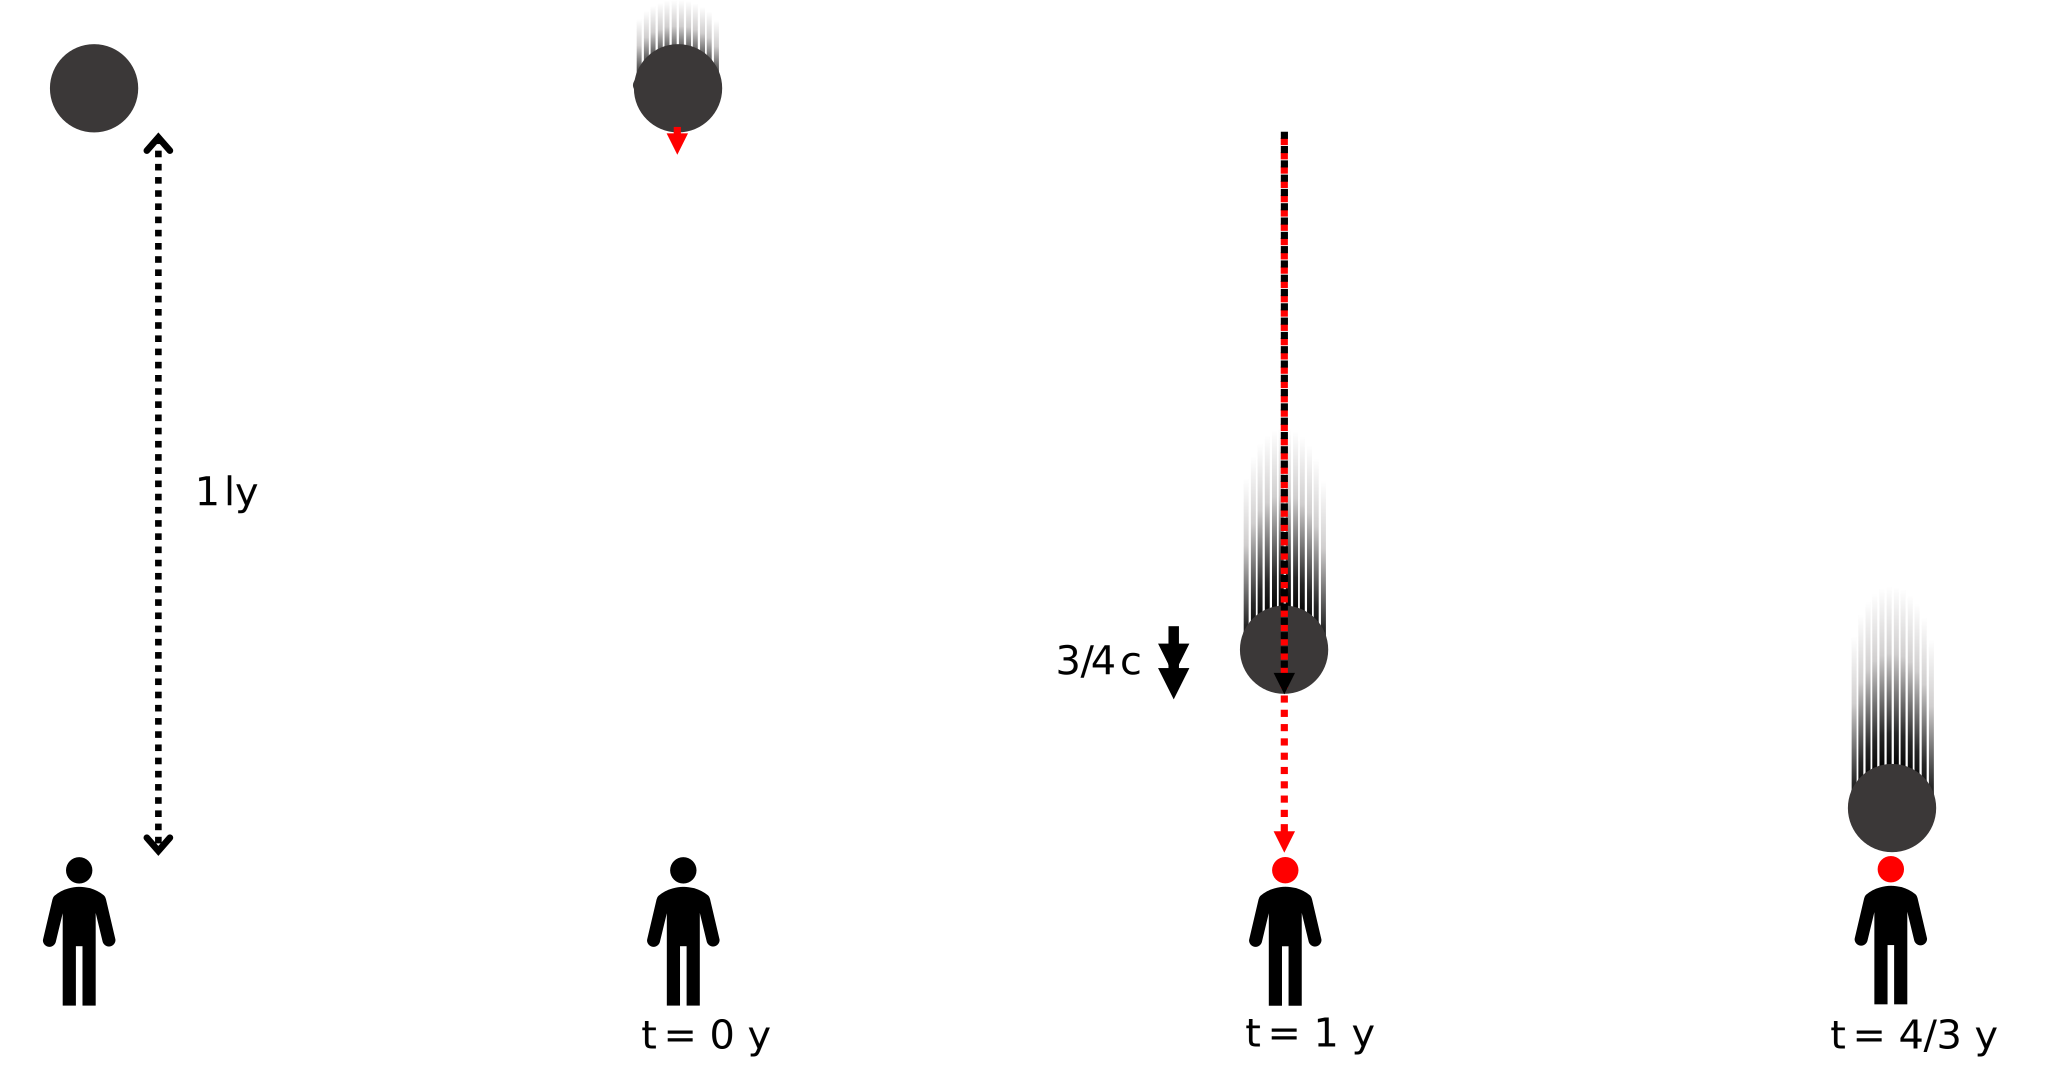
\includegraphics[width=10cm]{images/pdf/Perceived_speed.pdf}
	\caption{A diagram demonstrating the perceived speed of a ball vs its actual speed.}
	\label{fig: perceived vs actual speed}
\end{figure}
%███████████

This shows how important it is to consider the delay in the light from objects when observing relativistic systems.
This view is called the delayed/retarded view, meaning what we see now are objects in their past positions, and the further things are from us, the further into the past we are currently seeing them.

%*** Javascript can redo train diagrams but with speeds less than that of light and have the time between emission and absorption being identical, but speeds and direction of pulse changing depending on rest direction

%*** javascript Diagram could have an animated polar graph of how velocities change for low and fast velocities and frame changes *** could show classical addition of velocities in it too, either as an overlay, beside it, or using button

% Is there a way to visualize the change in none speed of light velocities

%███████████████████████████████████████████████████████████████████
%███████████████████████████████████████████████████████████████████
%\section{The More Abstract Properties...}% of Momentum, Energy and Mass}

%*** could talk about what happens to the quantities without saying why

%This also means that it is impossible to get any particle with mass up to the speed of light, as the closer the particle gets to the speed of light, the heavier it is perceived and, therefore, keeps requiring a greater and greater force to accelerate it, This amount of perceived mass tends to infinity and the force needed to accelerate it would also tend to infinity.\newline

%***
%(diagram)
%If we have two balls roll to the center of a train at rest and hit each other and stick, giving zero overall momentum as both ball's momentum cancels each other out, but to the observer on the track, the stuck-together balls move with the train, so the ball at the back of the train must have more momentum before the collision...
%*** So far, this is also true for classical frame transform

%From before, we have that the consequence of the different times and coordinates is that if a moving object emits light to allow the speed of light to stay constant, the transform will also have the consequence of changing the frequency of the light and hence its energy.

%Since energy is measured in units of position and time (as well as mass), the energy of a particle and systems in different frames have to go through transformations themselves, which leads to the famous energy and mass equivalence equation E=mc2 (this is the reduced form of the equation)\newline

%From finding how the momentum changes between 2 frames due to the Lorentz transformations, we see a relation between the mass of a particle and how much energy this particle is equivalent to. That is, if a particle with a certain mass annihilates with its anti-particle, it gives out photons, corresponding to the energy of the particle, which is different whether it is at rest or moving, as the perceived mass of a particle increases the faster it moves\newline

%███████████████████████████████████████████████████████████████████
%███████████████████████████████████████████████████████████████████
\section{Summary}

A key early concept was that light traveled through a medium called the luminiferous aether.
The Michelson-Morley experiment attempted to measure Earth's motion relative to this aether.
Surprisingly, no difference was found in the speed of light regardless of direction through this proposed aether.
This conflicted with the intuitive addition of velocities, discredited the aether theory, and led Einstein to propose light's constant speed in all inertial frames of reference as a fundamental principle.

Special relativity emerged from this insight that light's speed in a vacuum is constant for all observers, regardless of the light source's speed relative to each observer.
This required rethinking the concepts of time intervals and distances between points to accommodate light's fixed speed.
This led to the requirement that a clock moving relative to an observer ticks slower from the observer's perspective while also being contracted in the direction of its motion.
This was shown in Figure (\ref{fig: train clock}) and Figure (\ref{fig: full train transform}).
The faster an object moves relative to an observer, the more its lengths contract, and its time dilates to the observer.

It also led to the \hyperlink{def-simultaneity}{simultaneity} of events not being absolute.
For example, light emitted from the middle of a moving train reaches the front and back walls simultaneously for an observer at rest in the train.
But an observer standing still on the track sees the light hit both walls at different times, as shown in Figure (\ref{fig: train simultaneity}).
There is no universal "now" at a distance - observers relate times of events differently.

Classical physics provides an excellent approximation of reality at low speeds.
Relativistic effects only become readily noticeable at speeds approaching that of light.
We do not experience them because motions in everyday life are very slow relative to that of light, which is roughly three hundred million meters per second.

When it comes to velocities, they combine differently than in classical physics.
However, we must ensure that the transforms reduce to the intuitive addition of velocities of classical physics at low speeds while accommodating light's constant rate in all frames of reference.
This leads to initially bizarre outcomes like \textbf{apparent} faster-than-light motion emerging from how relativistic optical effects play out across distances, which is due to the delay in light signals from objects at a distance.
Nevertheless, special relativity gives a truer, more accurate picture of reality.

Due to space-time effects on wave propagation, we also have seen that the emitted light's frequencies shift (doppler effect) for a moving source that light is concentrated in the direction of the source's motion (aberrational effect).
Together, both intensely focus light in the direction of rapidly moving objects, giving relativistic beaming.

These effects will all be explained more fully with math in the coming chapters, along with other effects that require the math to fully understand, as well as new energy, mass, and momentum conservation laws.
We will derive everything step by step, starting with the transformation of positions and times between reference frames.



%███████████████████████████████████████████████████████████████████
%███████████████████████████████████████████████████████████████████

%*** observered vs apparent vs perceived vs retarded when it comes to velocity, time, arrival time, position


\newgeometry{top=1in, bottom=1in, left=1in, right=1in}
\setlength{\headwidth}{\textwidth}
%███████████████████████████████████████████████████████████████████
%███████████████████████████████████████████████████████████████████
\section{Definitions}
\begin{multicols}{2}

%██████████████████
\subsection*{\underline{Mathematical Framework}}

%
\term{def-Reference-frame}{Reference frame}{reference frame,frame of reference}{
An abstract coordinate system, consisting of three spatial and one time axis. The origin, orientation, and scale of its axis are specified by a set of points in space. The purpose of it is to provide a standardized means of defining the position and orientation of objects at any instant in time.}

%
\term{def-Inertial-reference-frame}{Inertial reference frame}{Inertial reference frame, Inertial frame of reference}{
A reference frame that is not undergoing any acceleration. An observer's reference frame is inertial if they do not feel a force acting on them.}

%
\term{def-proper-frame}{Proper/Rest frame}{proper frame,rest frame}{
This is the reference frame of the observer or object itself.}

%
\term{def-Primed-Frame}{Primed frame}{Primed frame,Prime frame}{
A reference frame that is moving relative to the current frame.}

%
\term{def-initial-Frame}{Initial frame}{initial frame}{
The first reference frame that we are comparing the current or primed reference frame to.}

%
\term{def-Moving-Frame}{Moving frame}{moving frame}{
An inertial reference frame that is moving relative to the rest frame.}

%
\term{def-frame-velocity}{frame velocity}{frame velocity}{
The velocity of a reference frame relative to the current reference frame.}

%
\term{def-transform}{Frame transform}{frame transform,frame transformation,transform,transformation}{
The changing of coordinates and other quantities in a reference frame into their corresponding values in another reference frame.}

%
\term{def-galilean-transform}{Galilean/Classical frame transform}{galilean,galilean transform,classical transform,Galilean frame transform,classical frame transform,classical tranformation}{
Transformation of coordinates and physical quantities according to Newtonian physics between two frames of reference.}

%
\term{def-lorentz-transform}{Relativistic frame transform}{Relativistic transform,Relativistic frame transform,Relativistic tranformation,lorentz transform,lorentz transformation}{
The changing of the spatial coordinates, the time coordinate, and other physical quantities into their corresponding values in a different inertial reference frame using equations from special relativity.}

%
\term{def-observer}{Observer}{observer}{
An entity/thing with an associated frame of reference/system of coordinates, with respect to which you can measure an object's position, orientation, shape, signal emission and other properties.}

%
\term{def-event}{Event}{event}{
An occurrence that can be specified by a unique combination of the three spatial and one time coordinates. These four coordinates, together, form a point in spacetime.}

%
\term{def-simultaneity}{Simultaneity}{simultaneous,simultaneity,simultaneously}{
Within a reference frame, two or more events are simultaneous if they occur at the same time within it. Classically, if any two events are simultaneous in one reference frame, they are also simultaneous in another. This is not true in special relativity, and the order of events can depend on the frame of reference.}

%
\term{def-retarded-position}{Retarded position}{retarded position}{
The previous position of a source, that an observer currently sees it at, due to the time delay between when a moving source emitting the signal and when the observer detects it.}

%██████████████████
\subsection*{\underline{The Mechanics}}

%
\term{def-aether}{Aether}{aether}{
A proposed medium that filled the vacuum of space that light propagated through.}

%
\term{def-vacuum}{Vacuum}{vacuum}{
Space that contains no matter.}

%
\term{def-length-contraction}{Lorentz length contraction}{lorentz length contraction,length contraction}{
The shortening of a moving object along the direction of its motion relative to an observer (compared to the length of object at rest).}

%
\term{def-time-dilation}{Time dilation}{time dilation}{
The slowing of the passing of time for objects in motion relative to an observer, compared to the passing of time for the observer.}

%
\term{def-doppler-effect}{Doppler effect}{doppler effect}{
The change of a wave's frequency due to the motion of its source relative to an observer. This is due to the bunching up of the wave in the direction of movement of the source and the stretching of the wave in the opposite direction, as well as the dilation of time between the emission of the crests of the emitted wave.}

%
\term{def-aberration}{Aberration of light}{aberration,aberrated,aberrate,aberrating,aberrates}{
The changing of the direction of the propagation of light when changing to another reference frame.}

%
\term{def-relativistic-beaming}{Relativistic beaming}{relativistic beaming,beaming}{
The accumulation of the Doppler effect and aberration of light, and how it affects the amount of light and its frequency emitted at different angles from a moving source. This effect can be extended to any wave or field emitted at the speed of light from a moving source.}

%
\term{def-retarded-field}{Retarded field}{retarded field}{
A moving source's field, where each point in the field has had its field propagated at the speed of light from the source's retarded position (i.e. the previous position of the source where it had emitted that part of the field from).}

%
\term{def-field}{Field}{field}{
A physical quantity that has a value (or a set of values) assigned to every point in space and time.}

%
\term{def-light-year}{Light year}{light year}{
The distance light travels in one year (in a vacuum).}

%██████████████████
\subsection*{\underline{Definitions for Later Chapters}}

%
\term{def-lorentz-invariant}{Lorentz Invariant/Frame independent}{invariant,lorentz invariant,transform invariant,transformation invariant,frame independent}{
A quantity or law of physics is Lorentz Invariant/Frame independent, if it remains unchanged when transforming coordinates and other quantities to any other inertial reference frame.}

%
\term{def-postulates}{Postulates}{postulate}{
A statement that is assumed to be true and is used as a basis for reasoning for a theory.}

%
\term{def-flux}{Flux}{flux}{
A measure of how much of a quantity is passing through a given surface in a given time (flowrate through a surface)}

%
\term{def-apparent-velocity}{Perceived/Apparent Velocity}{perceived velocity,apparent velocity}{
The velocity an object appears to have due to the time delay in the signal of light from it, as the time delay from each position along a sources path is different due to having different distances the signal needs to travel to observer (It is the consequence of the time difference in the propagation time of the light signal from the different positions of a source's path).}

%
\term{def-rest-mass}{Rest mass}{Rest mass,proper mass}{
The mass of a particle in its own rest frame}

%
\term{def-rest-mass-energy}{Rest mass energy}{Rest mass energy,rest energy, proper energy}{
The energy a particle has due to its rest mass (given by its rest mass times speed of light squared)}

\end{multicols}
\restoregeometry
\setlength{\headwidth}{\textwidth}

%███████████████████████████████████████████████████████████████████
%███████████████████████████████████████████████████████████████████
%███████████████████████████████████████████████████████████████████
\chapter{Positions, Time and Velocity} %The Math Begins:

Now that we have learned about the concepts of special relativity, we can let the mathematics begin, with classical relativity as a starting point, which will give us an understanding of how to \hyperlink{def-transform}{transform} between \hyperlink{def-Reference-frame}{reference frame}s.
We can then compare special relativity to this to help with our intuition.

%███████████████████████████████████████████████████████████████████
%███████████████████████████████████████████████████████████████████
\section{Classical Relativity}

For classical (Galilean) relativity, if we have two \hyperlink{def-observer}{observer}s moving relative to each other at constant velocity and want to find how each \hyperlink{def-observer}{observer} would describe the positions and motion of a particle relative to them, we need to know the positions and times in one observer's frame and how to \hyperlink{def-transform}{transform} them into the other \hyperlink{def-observer}{observer}s frame.
i.e.
if we have how one \hyperlink{def-observer}{observer} would describe the coordinates of a particle over time relative to them and we want to now know the coordinates of the particle with respect to the other \hyperlink{def-observer}{observer}, we need to know how the transformation of coordinates works.

Before special relativity, it was assumed that distances between two positions were the same for all \hyperlink{def-observer}{observer}s, i.e.
the first \hyperlink{def-observer}{observer} would see a stick and measure it to be the same length as another \hyperlink{def-observer}{observer} moving relative to them would measure it to be.
long story short, lengths are the same for all \hyperlink{def-observer}{observer}s in \hyperlink{def-galilean-transform}{Galilean transform}.
Another assumption is that time is constant for everyone, i.e.
clocks move at the same rate for each \hyperlink{def-observer}{observer} and if a particle was to emit light at a particular time.
This light would be emitted at the same time for the other \hyperlink{def-observer}{observer}s too.

So let us see how the mathematics works for the classical coordinate system transform between two \hyperlink{def-observer}{observer}s.
If we have the coordinate system in one \hyperlink{def-Inertial-reference-frame}{inertial reference frame} ${<\!\!S\!>}$ to describe an \hyperlink{def-event}{event} ${E}$, which is given by the set of spatial and time coordinates $({x},{y},{z})$ and ${t}$, and we want to find the coordinates of the event in another "primed" \hyperlink{def-Inertial-reference-frame}{inertial reference frame}/coordinate system that is moving at a relative speed $v$ to the first frame in the z-axis, that was initially overlapping with the first frame at time $t=0$, with the events coordinates now described by $x{'}, y{'}, z{'}$ at time $t{'}$.
The direction of the second frame is in the upwards z-direction instead of being to the right in the case of the truck diagrams from the previous chapter, this is to help us when we use spherical polar coordinates later and to help see the symmetries.

%█████████████
\begin{figure}[H]
	\figuretitle{...}
	\centering
	\tikzsetnextfilename{Tikz_simple_Galilean_transform_derivation}
	\begin{tikzpicture}[scale=3]%,tdplot_main_coords]
		\coordinate (O) at (0,0,0);
		%
		\draw (1.7,2,0) node{ {\large ${<\!\!S\!>}$}};
		\draw[black, thick,->] (1.5,0,0) -- (2.1,0,0) node[anchor=north east]{$x$};
		\draw[black, thick,->] (1.7,-0.2,0) -- (1.7,0.45,0) node[anchor=north west]{$z$};
		\draw[black, thick,->] (1.7,0,0.3) -- (1.7,0,-0.7) node[anchor=west]{$y$};
		%
		\draw[gray, dashed, thick,->] (1.5,1.2,0) -- (2.1,1.2,0) node[anchor=north east]{$x{'}$};
		\draw[gray, dashed, thick,->] (1.7,1,0) -- (1.7,1.7,0) node[anchor= west]{$z{'}$};
		\draw[gray, dashed, thick,->] (1.7,1.2,0.3) -- (1.7,1.2,-0.8) node[anchor=south]{$y{'}$};
		\draw[gray, thick, ->>] (1.55,1.2,0) -- (1.55,1.42,0) node[anchor=east]{$v$};
		\fill[red] (2.35,1.4,0) circle (0.6pt);
		%
		\draw[red, thick, ->] (1.7,0,0) -- (2.35,1.37,0) node[midway,anchor=west]{$\vec{OE}$};
		\draw[red, thick, ->] (1.7,0,0) -- (1.7,1.2,0) node[midway,anchor=east]{$\vec{OO{'}}$};
		\draw[red, thick, ->] (1.7,1.2,0) -- (2.32,1.4,0) node[midway,anchor=south]{$\vec{O{'}E}$};
		%
	\end{tikzpicture}
	\caption{Diagram, of a \protect\hyperlink{def-Reference-frame}{reference frame} ${<\!\!S\!>}$ with its associated $(x,y,z)$ coordinate system at rest in this frame, it also shows a primed coordinate axis $(x{'}, y{'}, z{'})$ at time $t=t{'}$ from when the axis where overlapping, associated with another \protect\hyperlink{def-Inertial-reference-frame}{inertial reference frame}s moving at velocity $v$ in the z-axis, it shows an \protect\hyperlink{def-event}{event} with position vector $\vec{OE}$ in this frame and the vector $\vec{OO{'}}$ to this primed axis origin and the vector $\vec{O{'}E}$ which is the vector from this primed origin to the \protect\hyperlink{def-event}{event} in the shown frame.}
	\label{fig: simple Galilean transform derivation}
\end{figure}
%███████████

For frame ${<\!\!S\!>}$ we have its origin ${O}$ and an \hyperlink{def-event}{event} ${E}$ located at

\begin{equation}
	\vec{OE}=(x,y,z)
\end{equation}

at time ${t}$ from axis overlap, and a prime frame ${<\!\!S{'}\!\!>}$'s origin $O{'}$ moving at relative velocity $v$ so that in the original frame we have after a time

\begin{equation}
	\vec{OO{'}}=(0,0,vt)
\end{equation}

in ${<\!\!S{'}\!\!>}$ we have the \hyperlink{def-event}{event}'s coordinates as

\begin{equation}
	\vec{O{'}E} = ( x{'}, y{'}, z{'} ) = \vec{OE} - \vec{OO{'}} = (x,y,z-vt)
	\label{eq: classical event}
\end{equation}

for frame ${<\!\!S\!>}$ we have

\begin{equation}
	\vec{OE} = (x,y,z) = \vec{OO{'}} + \vec{O{'}E} = (x{'},y{'},z{'}+vt{'})
	\label{eq: classical event 2}
\end{equation}

so we have $x=x{'}$, $y=y{'}$, $t=t{'}$ (time is assumed to be the same across reference frames in classical relativity), and for the z-components

\begin{equation}
	\begin{aligned}
		 & z{'} = z - vt \\
		 & z = z{'}+vt{'}
	\end{aligned}
\end{equation}

This shows the symmetry between the frames, as if we were originally in the ${<\!\!S{'}\!\!>}$ frame we would have the ${<\!\!S\!>}$ frame moving at -$v$ relative to it, so we would expect that the inverse \hyperlink{def-transform}{transformation} would replace one frame's coordinates with the other and have the opposite \hyperlink{def-frame-velocity}{frame velocity} instead.
So the inverse of going from \hyperlink{def-Primed-Frame}{primed frame} to original is just a matter of swapping all primed coordinates with original coordinates and changing the sign on the \hyperlink{def-frame-velocity}{frame velocity}, this can be seen from starting at time $t=0$ we have the frame's origins overlapping and that there is a symmetry from here, we have the freedom to choose either frame to be the original, as no frame is particularly special and depending which one you pick the relative velocity is either $v$ or -$v$.

The full description of the position and time \hyperlink{def-transform}{transform} for an \hyperlink{def-event}{event} is given as

\begin{equation}
	\begin{aligned}
		 & x{'}=x               \\
		 & y{'}=y               \\
		 & z{'} = z-vt          \\
		\text{at time \ \ \ } \\
		 & t{'}= t
	\end{aligned}
	\label{eq: Galilean transformation}
\end{equation}

%███████████████████████████████████████████████████████████████████
%███████████████████████████████████████████████████████████████████
\section{Postulates of Special Relativity}

\begin{tcolorbox}[breakable]
	\begin{enumerate}
		\item The laws of physics are the same in all \hyperlink{def-Inertial-reference-frame}{inertial frames of reference} (i.e.
if an \hyperlink{def-observer}{observer} carries out an experiment in an \hyperlink{def-Inertial-reference-frame}{inertial reference frame}, there would be no difference if the experiment was instead carried out within a different \hyperlink{def-Inertial-reference-frame}{inertial reference frame})
		\item The speed of light in a \hyperlink{def-vacuum}{vacuum} is the same in all inertial/non-accelerating frames of reference.
	\end{enumerate}
\end{tcolorbox}

They are not the only assumptions, you may notice some small jumps in the logic when it comes to the derivation.
But be aware small miss understandings have thrown people down the special relativity rabbit hole when trying to find inconsistencies or prove it wrong, throughout I will try to leave as few logical gaps as possible, and explain as simply and as in-depth as possible so that you do not do this yourself.

%███████████████████████████████████████████████████████████████████
%███████████████████████████████████████████████████████████████████
\section{Time Dilation}

%█████████████
\begin{figure}[ht]
	\figuretitle{...}
	\centering
	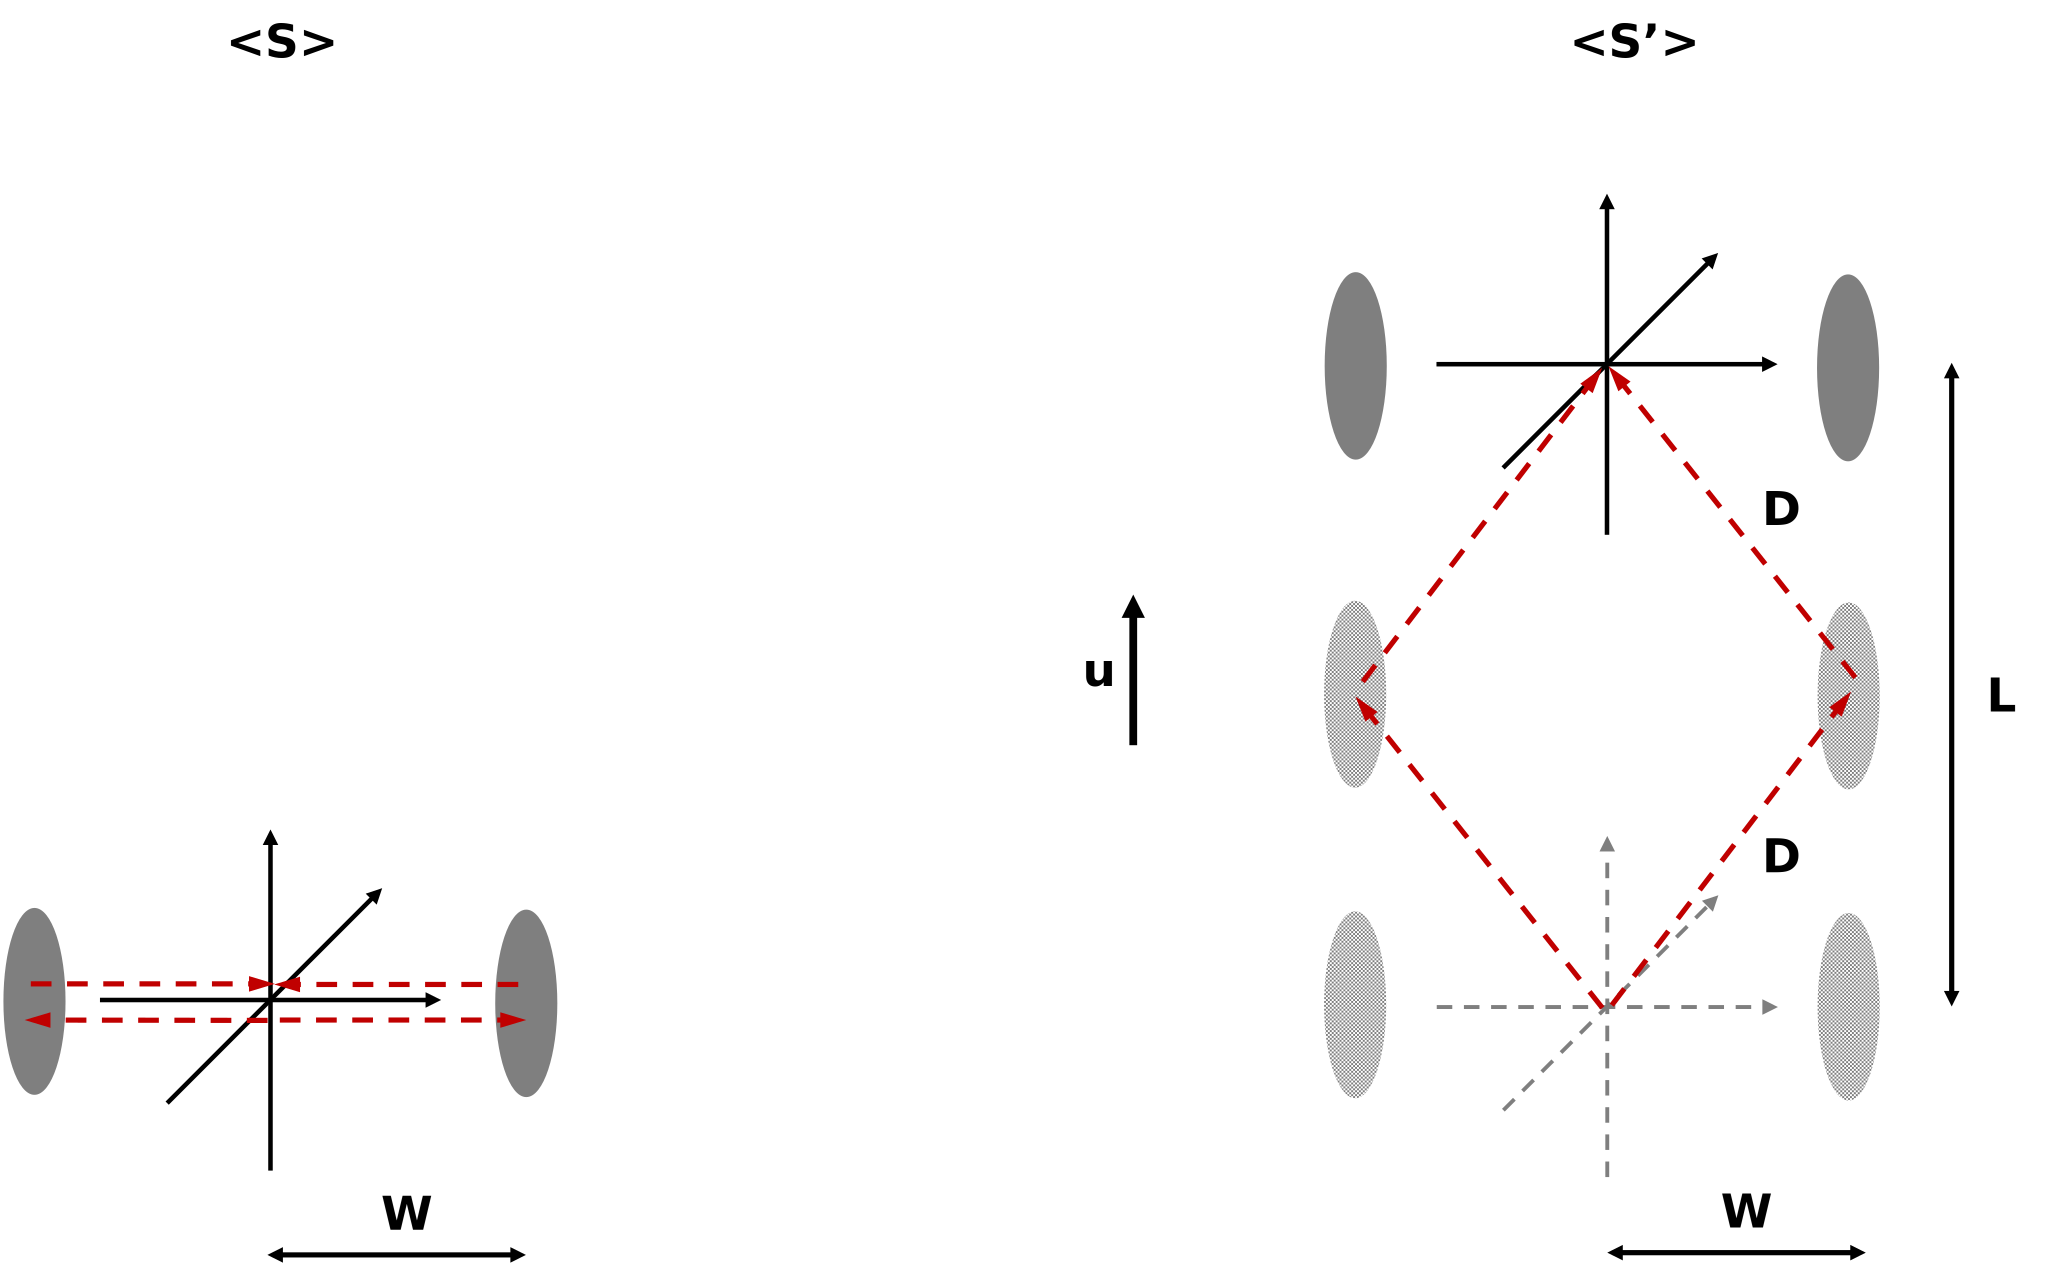
\includegraphics[width=10cm]{images/pdf/Light_clock.pdf}
	\caption{A diagram showing a clock keeping time using light, light is emitted from the origin and reflected off a mirror back to the origin, shown here in two different frames (describe what things are in the diagram)(need axis labels)}
	\label{fig: light clock}
\end{figure}
%███████████

We can have a clock that keeps time using a light pulse being emitted from a bulb towards a mirror and back again, recording a tick on its clock each time it returns to where it was emitted, taking a time $\Delta \tau$ in the rest frame to return.
The distance the light travels to the mirror and back in this time is

\begin{equation}
	2W=c\Delta \tau,
\end{equation}

the distance the bulb travels during this in the moving frame is

\begin{equation}
	L=u\Delta t{'} = -v \Delta t{'},
\end{equation}

where $\Delta t{'}$ is the time it took light to return in moving frame and $u$ is the speed of the bulb which is in the opposite direction of the \hyperlink{def-Primed-Frame}{primed frame} relative to the \hyperlink{def-proper-frame}{proper frame}, i.e.
$u=-v$, the distance light travels in this time is

\begin{equation}
	2D = c \Delta t{'},
\end{equation}

this forms a triangle, so we have the square of the hypotenuse $2D$ equal to the square of the lengths $W$ and $L$:

\begin{equation}
	c^2 \Delta t{'}^2 = v^2 \Delta t{'}^2 + c^2\Delta \tau^2
\end{equation}

rearranging to find the time it took in the \hyperlink{def-Primed-Frame}{primed frame} relative to the time in the \hyperlink{def-proper-frame}{proper frame}, we find

\begin{equation}
	\Delta t{'} = \dfrac{1}{\sqrt{1-\dfrac{v^2}{c^2}}} \Delta \tau = {\gamma} \Delta \tau
\end{equation}

with

\begin{equation}
	{\gamma} = \dfrac{1}{\sqrt{1-\dfrac{v^2}{c^2}}}.
\end{equation}

which means

\begin{equation}
	\Delta t{'} \geq \Delta \tau
\end{equation}

So we take this outcome as the time taken between two \hyperlink{def-event}{event}s in the same position in the moving frame taking longer than in the \hyperlink{def-proper-frame}{rest frame} of the clock, due to the longer distance it must travel at the same speed.

%███████████████████████████████████████████████████████████████████
%███████████████████████████████████████████████████████████████████
\section{Length Contraction TODO}

%█████████████
\begin{figure}[H]
	\figuretitle{...}
	\centering
	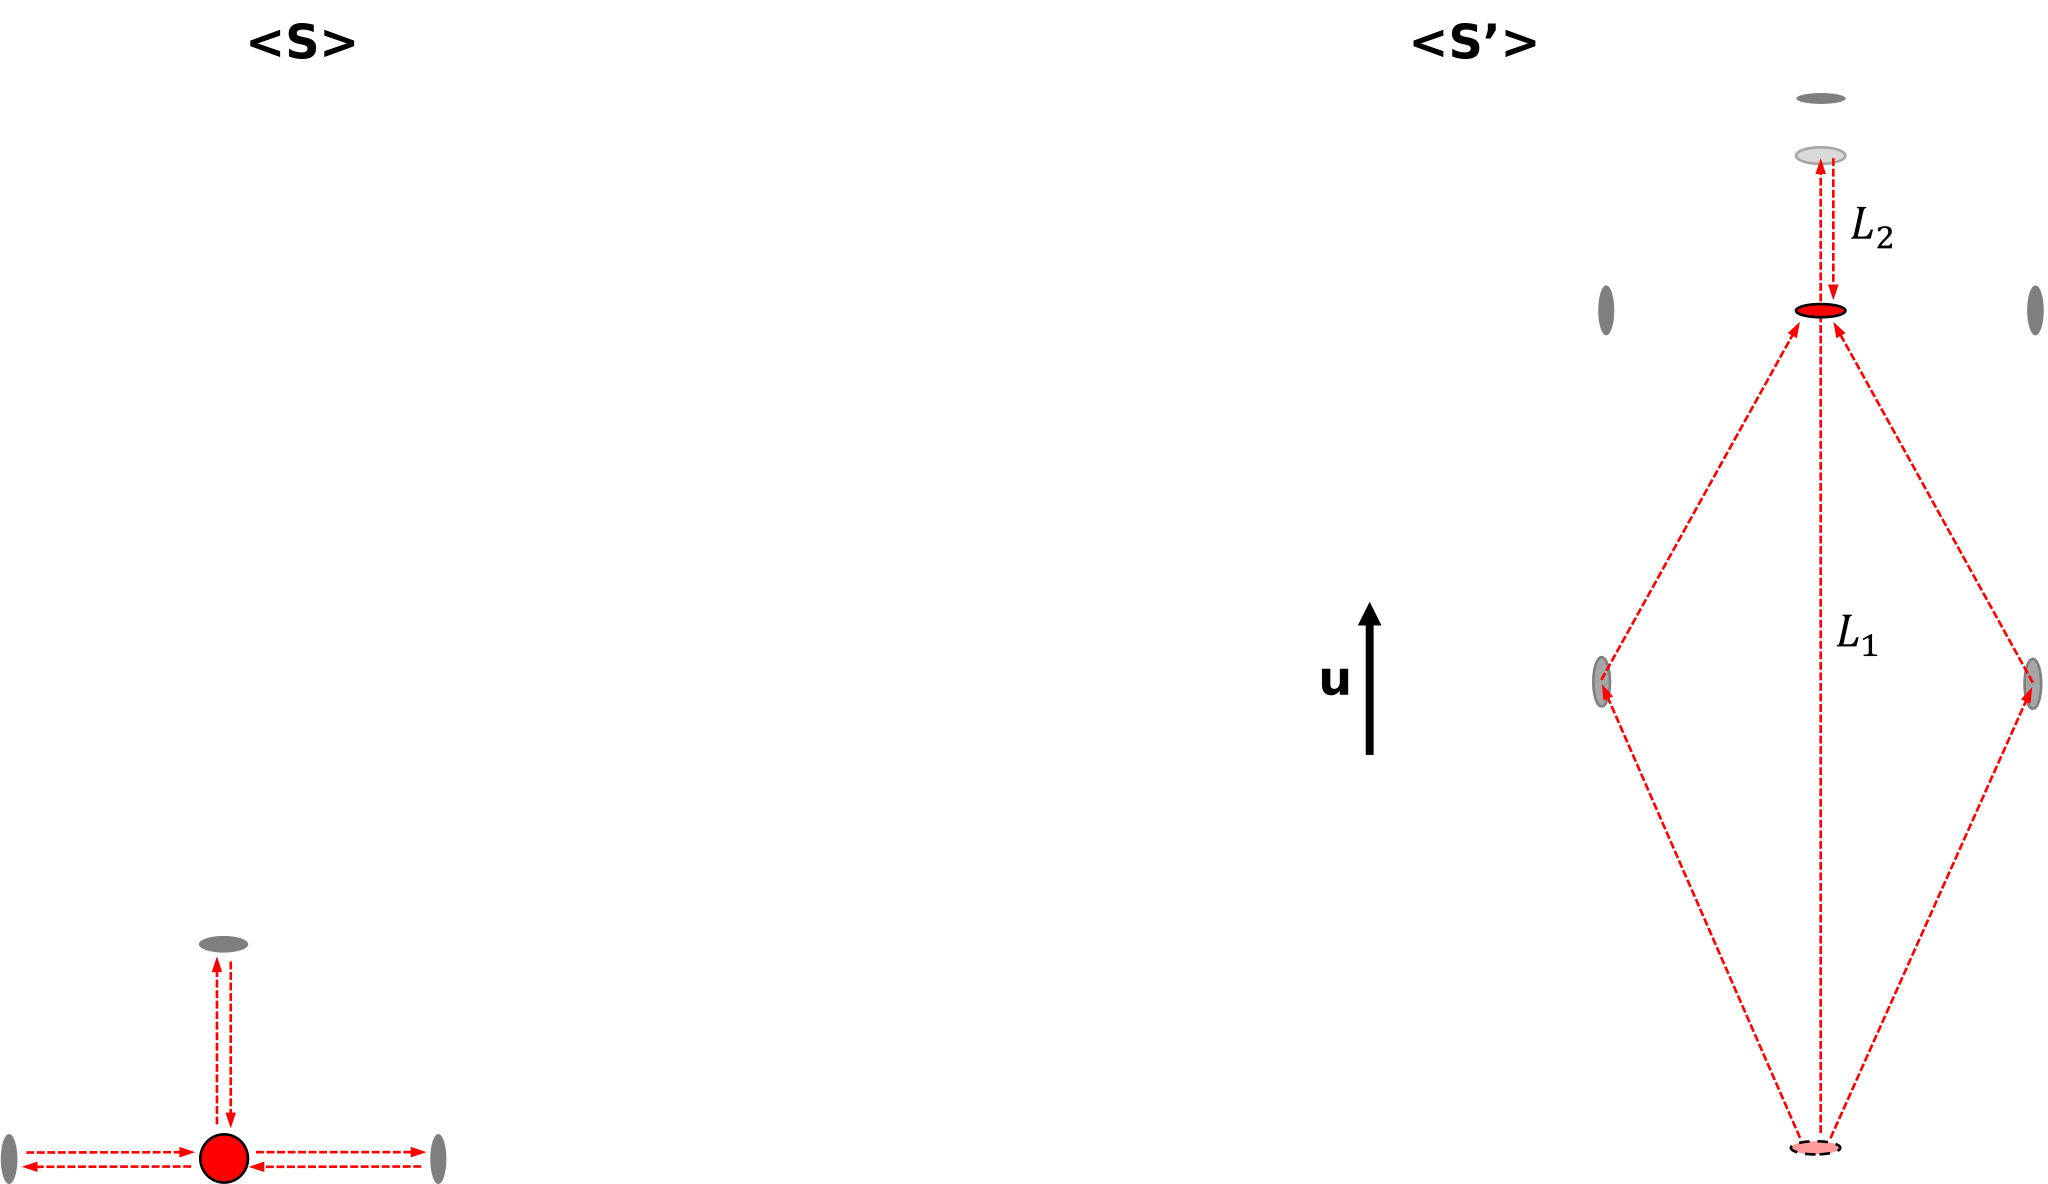
\includegraphics[width=10cm]{images/pdf/Length_Contraction.pdf}
	\caption{A diagram, showing a central bulb emitting light in the three directions, with all light being reflected by the mirrors back to the center, this is shown at rest on the left and moving in another inertial frame with the system now moving, with its length slightly contracted in the direction of movement.}
	\label{fig: length contraction math}
\end{figure}
%███████████

If we have a system in its rest frame with light emitted in three directions from the center, one directly in front and the other two to the sides, with equally distanced mirrors in the three directions so that they will be reflected back and return to the center simultaneously.
we require that in the moving frame they also all return to the center simultaneously, as multiple events that happen at a single point simultaneously in one frame, must happen simultaneously in all other frames.
This time between the light being emitted and absorbed will be the dilated time from the previous section.
To achieve this simultaneity in the return of the light to the bulb, the length of the full path of light from there center to the mirrors and back in each direction must be the same (as its speed of light is the same in all directions and the return time must be the same), we can work out the length of the sideways paths from the time dilation section, and this is the length the path needs to be in the vertical directions as well, the paths can only have this length if the system length is contracted when moving in the direction of movement.
Note that there is no contraction in the perpendicular direction to the movement due to the paradox explained in Figure (\ref{fig: width contraction}).

The pulse sent forward has a distance

\begin{equation}
	L_1= c{t}_1^{'}= D{'} + ut{'}_1
\end{equation}

to travel to get to the mirror that is moving away from the point it was emitted, where $t{'}_1$ is the time taken to get there and $D{'}$ is the distance between the mirror in front and the bulb and $u$ being the speed the bulb and mirrors are moving in the primed frame.
After this, the light then must travel back to the bulb a distance

\begin{equation}
	L_2 = ct{'}_2= D{'} - ut{'}_2
\end{equation}

where $t{'}_2$ is the time taken to return to the bulb from the mirror, both of these give the two times as

\begin{equation}
	t{'}_1=\frac{D'}{c-u}
\end{equation}

and

\begin{equation}
	t{'}_2=\frac{D'}{c+u}
\end{equation}

adding both times together gives the total primed time

\begin{equation}
	t{'} = D{'}(\frac{1}{c+u} + \frac{1}{c-u})=\frac{D'}{c}\frac{1}{1-u^2/c^2} =\frac{D'}{c}\frac{1}{1-v^2/c^2}={\gamma}^2 \frac{D'}{c}
\end{equation}

from the time dilation equation, we have

\begin{equation}
	ct{'}=c{\gamma} t = {\gamma} D = {\gamma}^2 D{'}
\end{equation}

and finally leading to the contracted distance to the front mirror in the primed frame being

\begin{equation}
	D{'} = \frac{1}{{\gamma}}D
\end{equation}

so we have

\begin{equation}
	D{'} \leq D
\end{equation}

we take from this that distances in the direction of movement of an object are contracted in its direction of movement compared to the rest frame of the object.

%███████████████████████████████████████████████████████████████████
%███████████████████████████████████████████████████████████████████
\section{Position and Time Transformation}

For the derivation of the coordinate transformation between two inertial frames, we will follow a similar line of thought as we did in the first chapter on the conceptual introduction.
For those who are curious, there is an alternative derivation using spherical light pulses given in Appendix \ref{spherical light pulse derivation}.

%█████████████
\begin{figure}[H]
	\figuretitle{...}
	\centering
	\tikzsetnextfilename{Tikz_simple_lorentz_transform_derivation}
	\begin{tikzpicture}[scale=3]%,tdplot_main_coords]
		\coordinate (O) at (0,0,0);
		%
		\draw (1.7,2,0) node{ {\large ${<\!\!S\!>}$}};
		\draw[black, thick,->] (1.5,0,0) -- (2.1,0,0) node[anchor=north east]{$x$};
		\draw[black, thick,->] (1.7,-0.2,0) -- (1.7,0.45,0) node[anchor=north west]{$z$};
		\draw[black, thick,->] (1.7,0,0.3) -- (1.7,0,-0.7) node[anchor=west]{$y$};
		%
		\draw[gray, dashed, thick,->] (1.5,1.2,0) -- (2.1,1.2,0) node[anchor=north east]{$x{'}$};
		\draw[gray, dashed, thick,->] (1.7,1,0) -- (1.7,1.7,0) node[anchor= west]{$z{'}$};
		\draw[gray, dashed, thick,->] (1.7,1.2,0.3) -- (1.7,1.2,-0.8) node[anchor=south]{$y{'}$};
		\draw[gray, thick, ->>] (1.55,1.2,0) -- (1.55,1.42,0) node[anchor=east]{$v$};
		\fill[red] (2.35,1.4,0) circle (0.6pt);
		%
		\draw[red, thick, ->] (1.7,0,0) -- (2.35,1.37,0) node[midway,anchor=west]{$\vec{OE}$};
		\draw[red, thick, ->] (1.7,0,0) -- (1.7,1.2,0) node[midway,anchor=east]{$\vec{OO{'}}$};
		\draw[red, thick, ->] (1.7,1.2,0) -- (2.32,1.4,0) node[midway,anchor=south]{$\vec{O{'}E}$};
		%
	\end{tikzpicture}
	\caption{A diagram showing an \protect\hyperlink{def-event}{event} in a frame with another primed frame's axis shown moving in the z-direction.}
	\label{fig: simple Lorentz transform derivation}
\end{figure}
%███████████

If we are in a frame ${<\!\!S\!>}$ with origin $O$ at position $(0,0,0)$ and a primed frame ${<\!\!S{'}\!\!>}$ moving in the z-direction at velocity $v$ such that the position of the primed origin in this frame is

\begin{equation}
	\vec{OO{'}}=(0,0,vt)
\end{equation}

at time ${t}$ from when the origins overlapped, if there is an \hyperlink{def-event}{event} (let us say light or another object reaching a mirror that is moving with the \hyperlink{def-Primed-Frame}{primed frame}s axis) described in this frames coordinates as

\begin{equation}
	E = (x,y,z,t)
\end{equation}

with the spatial coordinates shown in the diagram as

\begin{equation}
	\vec{OE}=(x,y,z)
\end{equation}

in the primed frame we have the event described as

\begin{equation}
	E{'} = (x{'},y{'},z{'},t{'})
\end{equation}

now in the current frame, we have the \hyperlink{def-Primed-Frame}{primed frame}'s axis moving with the mirror, from the previous chapter we should have this primed distance in the z-direction to the event contracted, as the primed z-coordinates are contracted in this frame, as seen from length contraction section; the events z-coordinate is $z=z{'}/{\gamma}$, so that distance between the primes origin and the event in this frame (not the primed frame) is

\begin{equation}
	\vec{O{'}E} = (x,y,z{'}/{\gamma})
\end{equation}

noting that we have the x and y-components unaffected due to the cannon and ball thought experiment from the first chapter.
From the diagram, we can see

\begin{equation}
	\vec{OE}= \vec{OO{'}} + \vec{O{'}E}
	\label{eq: event}
\end{equation}

subbing each component into this equation for the z-direction and rearranging, we have

\begin{equation}
	z{'} = {\gamma} (z-vt)
\end{equation}

If we were instead in frame ${<\!\!S{'}\!\!>}$ we would have $\vec{OE}=(x,y,z/{\gamma})$, $\vec{OO{'}}=(0,0,vt{'})$, and $\vec{O{'}E} = (x,y,z{'})$, doing the same for these we have

\begin{equation}
	z = {\gamma} (z{'}+vt{'})
\end{equation}

This should be expected as this shows the expected symmetry between the frames because if we were originally in the ${<\!\!S{'}\!\!>}$ frame we would have the ${<\!\!S\!>}$ frame moving instead at -$v$ in the z-direction relative to the ${<\!\!S{'}\!\!>}$ frame, so we would expect that the inverse \hyperlink{def-transform}{transformation} would replace one frame's coordinates with the other and have the negative of the velocity instead.
Now substituting the z transforms into each other we have

\begin{equation}
	z = {\gamma} ( {\gamma} (z-vt)+vt{'})
\end{equation}

and rearranging gives

\begin{equation}
	t{'} = {\gamma} \left( \left( \dfrac{1}{{\gamma}^2}-1 \right)\frac{z}{v} + t \right)
\end{equation}

with ${\gamma}^{-2}=1-v^2/c^2$ then giving

\begin{equation}
	t{'} = {\gamma} \left( t - \dfrac{vz}{c^2} \right)
\end{equation}

leaving full description of the location and time of an \hyperlink{def-event}{event} as

\begin{equation}
	\mhl{
		\begin{aligned}
			 & x{'}=x                                           \\
			 & y{'}=y                                           \\
			 & z{'} = {\gamma} (z-vt)                           \\
			\text{at time \ \ \ }                             \\
			 & t{'}={\gamma} \bigg(t-\frac{vz}{c^2}\bigg)       \\
			\text{with \ \ \ }                                \\
			 & {\gamma} = \dfrac{1}{\sqrt{1-\frac{v^2}{c^2}}}
		\end{aligned}
	}
	\label{eq: Lorentz transformation}
\end{equation}

For the time \hyperlink{def-transform}{transform} the $\frac{vz}{c^2}$ term is the cause of \hyperlink{def-simultaneity}{simultaneous} \hyperlink{def-event}{event}s in one inertial frame no longer being \hyperlink{def-simultaneity}{simultaneous} in another inertial frame, and the gamma factor ${\gamma}$, is the term that causes the overall change in how fast time flows relative in each frame.
In the spatial coordinate transforms the gamma factor is the cause of the change of lengths in the direction of the frame's movement.
How the transformation works is shown in Figure (\ref{fig: coordinate transform}).

%█████████████
\begin{figure}[H]
	\figuretitle{...}
	\centering
	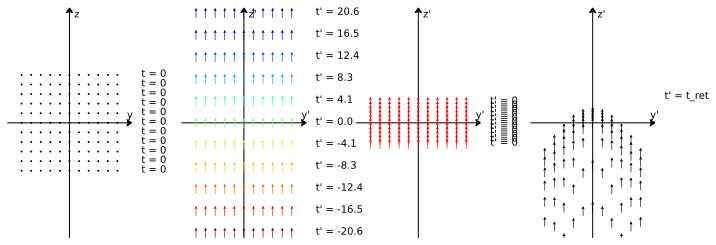
\includegraphics[width=10cm]{images/pdf/coordinate_transforms.pdf}
	\caption{A diagram, showing a grid of points at time $t=0$ that are at rest in their proper frame (left), giving the direct transformation into the moving primed frame (middle) where the points are now moving in the negative z-direction with the colors and labels showing the desynchronization of the primed times $t{'}$, the next figure (right) shows what these points would be when they are synchronized with the origin's time $t{'}=0$. *** split plots into several svgs and for other set later too, also call first picture "initial" frame of reference and others primed}
	\label{fig: coordinate transform}
\end{figure}
%███████████

%███████████████████████████████████████████████████████████████████
\subsection{Infinitesimal Changes of Coordinates}

\begin{equation}
	\begin{aligned}
		 & x{'}_2 - x{'}_1 = x_2 - x_1                                                                                   \\
		 & y{'}_2 - y{'}_1 = y_2 - y_1                                                                                   \\
		 & z{'}_2 - z{'}_1 = {\gamma} ( z_2 - v {t}_2) - {\gamma} ( z_1 - v {t}_1)                                           \\
		 & t{'}_2 - t{'}_1={\gamma} \bigg( {t}_2-\frac{v}{c^2} z_2 \bigg) - {\gamma} \bigg( {t}_1 - \frac{v}{c^2} z_1 \bigg)
	\end{aligned}
\end{equation}

leads to

\begin{equation}
	\label{eq: interval of Coordinates}
	\begin{aligned}
		 & \Delta x{'}= \Delta x                                              \\
		 & \Delta y{'}= \Delta y                                              \\
		 & \Delta z{'} = {\gamma} ( \Delta z-v \Delta t)                      \\
		 & \Delta t{'}={\gamma} \bigg( \Delta t-\frac{v}{c^2} \Delta z \bigg)
	\end{aligned}
\end{equation}

when taken the changes are infinitesimal this gives the differential quantities

\begin{equation}
	\label{eq: Infintesmal interval of Coordinates}
	\begin{aligned}
		 & dx{'}=dx                                        \\
		 & dy{'}=dy                                        \\
		 & dz{'} = {\gamma} (dz-vdt)                       \\
		 & dt{'}={\gamma} \bigg(dt-\frac{v}{c^2} dz \bigg)
	\end{aligned}
\end{equation}

%███████████████████████████████████████████████████████████████████
\subsection{Transforms with Low Relative Frame Speed Change}

For the coordinate transforms in the previous section we get back the classical \hyperlink{def-galilean-transform}{coordinates transform} for frame velocities much smaller than the speed of light, i.e.
with $v\ll c$ we have ${\gamma} \approx 1$ we get

\begin{equation}
	t{'} \approx t
\end{equation}

\begin{equation}
	z{'} \approx z - vt
\end{equation}

which is the expected result for the \hyperlink{def-galilean-transform}{classical coordinates transform}, and what we are used to seeing things work in everyday life.
The influence of the gamma factor is shown in Figure (\ref{fig: Gamma Factor}).

%█████████████
\begin{figure}[H]
	\figuretitle{...}
	\centering
	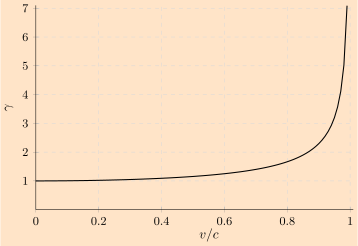
\includegraphics[width=10cm]{images/pdf/Gamma_Factor.pdf}
	\caption{A diagram, showing the magnitude of the gamma factor with increasing ratio of frame speed to the speed of light, with ${\gamma}$ tending to infinity as $v/c\rightarrow 1$.}
	\label{fig: Gamma Factor}
\end{figure}
%███████████

%███████████████████████████████████████████████████████████████████
%███████████████████████████████████████████████████████████████████
\section{Velocity}

from taking the infinitesimals of equations from eq.
\eqref{eq: Lorentz transformation}, we have the velocities as

\begin{equation}
	\begin{aligned}
		 & {{u}_{x}}^{'} = \frac{dx{'}}{dt{'}}=\frac{dx}{{\gamma} \bigg(dt-\frac{vdz}{c^2}\bigg) }                  \\
		 & {{u}_{y}}^{'} = \frac{dy{'}}{dt{'}}=\frac{dy}{{\gamma} \bigg(dt-\frac{vdz}{c^2}\bigg) }                  \\
		 & {{u}_{z}}^{'} = \frac{dz{'}}{dt{'}} = \frac{{\gamma} (dz-vdt)}{{\gamma} \bigg(dt-\frac{vdz}{c^2}\bigg) }
	\end{aligned}
\end{equation}

now dividing the top and bottom of the fraction by $dt$ we can give the equations in their vector form as

\begin{equation}
	\label{eq: velocity transform}
	\mhl{
		\begin{aligned}
			 & \mathbf{U}{'} = \dfrac{1}{{\gamma}\left(1- \dfrac{v}{c^2} {{u}_{z}}\right) }
			\begin{pmatrix}
				{{u}_{x}}                             \\
				{{u}_{y}}                             \\
				{\gamma} \left( {{u}_{z}} - v \right) \\
			\end{pmatrix}
			\\
			 & \text{at position $\mathbf{R}{'}$ and time $t{'}$ }
		\end{aligned}
	}
\end{equation}

the generalized velocity \hyperlink{def-transform}{transform} derived in appendix (todo) is

\begin{equation}
	\mathbf{U}{'} = \dfrac{1}{{\gamma}} \dfrac{\mathbf{u}_s + \Big[\dfrac{{\gamma}-1}{\|\mathbf{V}\|^2}(\mathbf{u}_s\cdot \mathbf{V})- {\gamma} \Big] \mathbf{V}}{1 - \dfrac{\mathbf{u}_s\cdot\mathbf{V}}{c^2}}
\end{equation}

with $\mathbf{V}$ being the frame's velocity in any generalized direction, instead of just being in the z-direction

%███████████████████████████████████████████████████████████████████
%███████████████████████████████████████████████████████████████████
\section{Acceleration}

To find how the acceleration of a particle transforms for an \hyperlink{def-observer}{observer} in two different frames we take the differential of the velocity \hyperlink{def-transform}{transform} eq.
\eqref{eq: velocity transform} and use the differentiation rules for two generic functions $f$ and $g$: $d(gf)=f dg+g df$, and $d[f(g(x))]= dg(x) * df(g(x))$

\begin{equation}
	\begin{aligned}
		d\mathbf{U}{'} & = \dfrac{1}{{\gamma}\left(1- \dfrac{v}{c^2} {{u}_{z}}\right) }
		\begin{pmatrix}
			d{{u}_{x}}          \\
			d{{u}_{y}}          \\
			{\gamma} d{{u}_{z}} \\
		\end{pmatrix}
		+ \dfrac{{\gamma} \dfrac{v}{c^2} d{{u}_{z}}}{{\gamma}^2\left(1- \dfrac{v}{c^2} {{u}_{z}}\right)^2 }
		\begin{pmatrix}
			{{u}_{x}}                             \\
			{{u}_{y}}                             \\
			{\gamma} \left( {{u}_{z}} - v \right) \\
		\end{pmatrix}                                           \\
		             & = ...
                                                     \\
		             & = \dfrac{1}{{\gamma}\left(1- \dfrac{v}{c^2} {{u}_{z}}\right)^2 }
		\begin{pmatrix}
			d{{u}_{x}} + \frac{v}{c^2}( {{u}_{x}} d{{u}_{z}} - {{u}_{z}} d{{u}_{x}}) \\
			d{{u}_{y}} + \frac{v}{c^2}( {{u}_{y}} d{{u}_{z}} - {{u}_{z}} d{{u}_{y}}) \\
			\frac{1}{{\gamma}} d{{u}_{z}}                    \\
		\end{pmatrix}
	\end{aligned}
\end{equation}

Now, divide by the time differential from the previous chapter to get the acceleration transform

\begin{equation}
	\mhl{
		\begin{aligned}
			\mathbf{a}{'} = \dfrac{1}{{\gamma}^2\left(1- \dfrac{v}{c^2} {{u}_{z}}\right)^3 }
			\begin{pmatrix}
				{{a}_{x}} + \frac{v}{c^2}({{u}_{x}} {{a}_{z}} - {{u}_{z}} {{a}_{x}}) \\
				{{a}_{y}} + \frac{v}{c^2}({{u}_{y}} {{a}_{z}} - {{u}_{z}} {{a}_{y}}) \\
				\frac{1}{{\gamma}} {{a}_{z}}                 \\
			\end{pmatrix}
			\\
			\text{at position $\mathbf{R}{'}$ and time $t{'}$ }
		\end{aligned}
	}
\end{equation}

%███████████████████████████████████████████████████████████████████
\subsection{Generalized Acceleration Transform}

3 acceleration (check this)

\begin{equation}
	\mathbf{a{'}} = \frac{1}{{\gamma} ^3 \left(1-\frac{(\mathbf{u}\cdot \mathbf{v})}{c^2}\right)^3}\left[ {\gamma} \left(1-\frac{(\mathbf{u}\cdot\mathbf{v})}{c^2}\right)\mathbf{a}+\frac{{\gamma} (\mathbf{a}\cdot\mathbf{v})}{c^2}\mathbf{u} + (1-{\gamma} ) (\mathbf{a}\cdot\hat{\mathbf{v}}) \cdot\hat{\mathbf{v}}\right]
\end{equation}

at position $\mathbf{R}{'}$ and time $t{'}$

%███████████████████████████████████████████████████████████████████
%███████████████████████████████████████████████████████████████████
\section{ch3-Variables}

\noindent ... \newline

\noindent ... \newline


%███████████████████████████████████████████████████████████████████
%███████████████████████████████████████████████████████████████████
%███████████████████████████████████████████████████████████████████
\chapter{Observers Delayed World View}

Light travels extremely fast (roughly 300,000,000 m/s) compared to other everyday speeds we are used to.
In the blink of an eye, light could travel around the world twice.
We do not need to normally worry about the delay in the light signal, as the time to propagate the distances in our everyday world is very short, so the signal can be approximated as being instantaneous, therefore ignoring the more complex modeling of the delayed signal.
But when it comes to particle physics or astronomy, we might be dealing with speeds close to that of light or also huge distances, e.g.
light has taken 152,000 years to travel from the Andromeda galaxy, so we are currently seeing this galaxy where it was and how it looked 152,000 years ago.
These past positions that we currently see are called the \hyperlink{def-retarded-position}{retarded position}s/delayed view positions.

%███████████████████████████████████████████████████████████████████
%███████████████████████████████████████████████████████████████████
\section{Relativistic Observers Delayed view}

*** change $\theta_c$ to $\alpha$

When looking at moving objects we see them where they were in their past positions, due to the delay in the light signal, so let us talk about the \hyperlink{def-transform}{transform} showing a source particle emitting a photon to an \hyperlink{def-observer}{observer}, showing the \hyperlink{def-retarded-position}{retarded position} the \hyperlink{def-observer}{observer} sees.

%█████████████
\begin{figure}[ht]
	\figuretitle{...}
	\begin{subfigure}[b]{.49\textwidth}
		\tikzsetnextfilename{Tikz_Particles_position_in_rest_frame}
		\begin{tikzpicture}[scale=5] %[,tdplot_main_coords]
			%\usetikzlibrary{arrows.meta}
			\draw[thick] (0,0) circle (0.025);
			\draw[black, thick,->] (0,0,0) -- (0.4,0,0) node[anchor=north east]{$y$};
			\draw[black, thick,->] (0,0,0) -- (0,0.4,0) node[anchor=north east]{$z$};
			\draw[black, thick,->] (0,0,0) -- (0,0,0.55) node[anchor=south east] {$x$};
			\draw[gray,dashed, thick,->] (0,0,0) -- (0.2,0,0) node[anchor=north east]{$y{'}$};
			\draw[gray,dashed, thick,->] (0,0,0) -- (0,0.2,0) node[anchor=north east]{$z{'}$};
			\draw[gray,dashed, thick,->] (0,0,0) -- (0,0,0.35) node[anchor=south] {$x{'}$};
			\draw[gray, thick,,->>] (-0.15,0,0) -- (-0.15,0.1,0) node[anchor=north east]{$v$};
			\draw[->] (0,0.25/2,0) to[bend left=45] (0.19/2,0.18/2,0);
			\node at (0.08,0.17,0) {$\theta_{\scalebox{0.5}{R} } $};
			\draw[red, thick, dotted,<-] (0.02,0.02,0) -- (0.47,0.46,0) node[midway,right] {\text{ $\mathbf{R}_{p}$}}; % Reduced by 0.02
			\fill[blue] (0.49,0.48,0) circle (0.4pt) node[anchor=east] {\text{ $\mathbf{R}$}}; % Reduced by 0.02
			\draw[gray,dashed] (0.49,0.48,0) -- (0.49,0.65,0); % Reduced by 0.02
			\draw[->] (0.49,0.58,0) arc (90:-135:0.1);
			\node at (0.54,0.47,0) {$\theta_c $};
		\end{tikzpicture}
		\caption{Source and \hyperlink{def-observer}{observer}'s \hyperlink{def-proper-frame}{rest frame}}
		% \label{fig:sub1}
	\end{subfigure}
	\begin{subfigure}[b]{.49\textwidth}
		\tikzsetnextfilename{Tikz_Particles_position_in_primed_frame_with_delayed_position}
		\begin{tikzpicture}[scale=5] %[,tdplot_main_coords]
			%\usetikzlibrary{arrows.meta}
			\draw[thick] (0,0) circle (0.025);
			\draw[gray,	thick, dashed] (0,0.7,0) circle (0.03);
			\draw[blue,thick,dotted,->] (0.47,0.9,0) -- (0.47,0.22,0); %node[midway,left]{\textcolor{black}{ $\mathbf{P}{'}$}}; %$\mathbf{P}{'}$}}; % Reduced by 0.02
			\draw[gray,dashed, thick,->] (0,0.7,0) -- (0.2,0.7,0) node[anchor=north east]{$y$};
			\draw[gray,dashed, thick,->] (0,0.7,0) -- (0,0.9,0) node[anchor=north east]{$z$};
			\draw[gray,dashed, thick,->] (0,0.7,0) -- (0,0.7,0.35) node[anchor=south] {$x$};
			\draw[gray,dashed, thick,->] (0,0,0) -- (0.2,0,0) node[anchor=north east]{$y$};
			\draw[gray,dashed, thick,->] (0,0,0) -- (0,0.2,0) node[anchor=north east]{$z$};
			\draw[gray,dashed, thick,->] (0,0,0) -- (0,0,0.35) node[anchor=south] {$x$};
			\draw[thick,->] (0,0,0) -- (0.4,0,0) node[anchor=north east]{$y{'}$}; % Reduced by 0.02
			\draw[thick,->] (0,0,0) -- (0,0.4,0) node[anchor=north east]{$z{'}$};
			\draw[thick,->] (0,0,0) -- (0,0,0.55) node[anchor=south east] {$x{'}$};
			%\draw[gray,->] (0,0.25,0) to[bend left=40] (0.15,0.2,0);
			\draw[red, thick, dotted,<-] (0.02,0.02,0) -- (0.45,0.88,0) node[midway, right] {$\mathbf{R}_{p}^{'}$}; % Reduced by 0.02
			\draw[gray, thick, dotted,->] (0,0.7,0) -- (0,0.02,0);
			\fill[gray] (0.47,0.9,0) circle (0.4pt); % Reduced by 0.02
			\fill[blue] (0.47,0.2,0) circle (0.4pt) node[right] {\text{ $\mathbf{R}_{t{'}=0}^{'}$}}; % Reduced by 0.02
			\draw[thick,->>] (0,0.58,0) -- (0,0.49,0) node[midway,right]{$-v$};
			\draw[ thick,->>] (0.47,0.58,0) -- (0.47,0.49,0) node[midway,right]{$-v$}; % Reduced by 0.02
			\draw[gray,dashed] (0.47,0.9,0) -- (0.47,1.07,0); % Reduced by 0.02
			\draw[->] (0.47,1,0) arc (90:-120:0.1); % Reduced by 0.02
			\node at (0.52,0.91,0) {$\theta_{c}^{'}$}; % Reduced by 0.02
			\node[gray] at (0.72,0.91,0) {$\mathbf{R}_{t{'}=t{'}_{e}}^{'}$}; % Reduced by 0.02
		\end{tikzpicture}
		\caption{\hyperlink{def-Primed-Frame}{primed frame}}
		% \label{fig:sub2}
	\end{subfigure}
	\caption{Diagram of a source particle (blue) emitting light (red), which is absorbed by an \protect\hyperlink{def-observer}{observer} positioned at the origin at time $t=t{'}=0$ with the \protect\hyperlink{def-observer}{observer} and source at rest in the first inertial frame (left) and then shown moving in a \protect\hyperlink{def-Primed-Frame}{primed frame} (right).}
	\label{fig: Retarded field}
\end{figure}
%███████████

\noindent
\textbf{system:} \newline
If we take the \hyperlink{def-proper-frame}{rest frame} of an \hyperlink{def-observer}{observer} and a particle that emits a pulse of light from its position at $\mathbf{R}$ so that it is received by the \hyperlink{def-observer}{observer} at the origin, at time $t=0$.

The time the pulse of light was emitted is ${T}_{e}= -\frac{|\mathbf{R}|}{c}$ (were $\frac{|\mathbf{R}|}{c}$ is the time it takes light to propagate along $\mathbf{R}$ to the origin), and the velocity of that light that is propagating towards the origin is

\begin{equation}
	\mathbf{c} = c
	\begin{pmatrix}
		0              \\
		\sin{\theta_c} \\
		\cos{\theta_c} \\
	\end{pmatrix}
\end{equation}

giving the emitted position as

\begin{equation}
	\mathbf{R} = c {T}_{e}
	\begin{pmatrix}
		0              \\
		\sin{\theta_c} \\
		\cos{\theta_c} \\
	\end{pmatrix}
\end{equation}

the position vector and light's velocity are in opposite directions which can be seen due to the emitted time being negative.
If you wish to have this in terms of the position vector angle from the z-axis you can use the equation for the angles $\theta_{\scalebox{0.5}{R}} = \theta_c - \pi$.
Now inputting the delayed positions and times (with origin time $t=0$) in the first frame into the coordinate transform we get the delayed position in the primed frame as

\begin{equation}
	\begin{aligned}
		\mathbf{R}{'}     & = c{T}_{e}
		\begin{pmatrix}
			0                                                    \\
			\sin{\theta_c}                                       \\
			{\gamma} \left( \cos{\theta_c} - \frac{v}{c} \right) \\
		\end{pmatrix}
		=
		\begin{pmatrix}
			0                                    \\
			{{R}_{y}}                                  \\
			{\gamma} \left( {{R}_{z}} - {v} {{T}_{e}} \right) \\
		\end{pmatrix}
		\\
		\text{at time } &
		\\ {{t}{'}_{e}} & = {\gamma} (1-\frac{v}{c} \cos{\theta_{c}} ) {{T}_{e}}
	\end{aligned}
\end{equation}

we can see that this does agree with the light's velocity \hyperlink{def-transform}{transform} as well, as it is in the direct opposite direction to $\mathbf{R}$ as it should be.
With the light being received at the origin of the \hyperlink{def-Primed-Frame}{primed frame} axis at time $t{'}=0$, this is the delayed position, if you wanted to find the position of where the particle actually is, we would need to propagate this to the current time of zero of the observer, given by

\begin{equation}
	\mathbf{R}_{t{'}=0}^{'} = \mathbf{R}{'} - \mathbf{v}t{'}_{e} = c{T}_{e}
	\begin{pmatrix}
		0                                 \\
		\sin{\theta_c}                    \\
		\frac{1}{{\gamma}} \cos{\theta_c} \\
	\end{pmatrix}
\end{equation}

%███████████████████████████████████████████████████████████████████
%███████████████████████████████████████████████████████████████████
\section{Delayed View of Transformed Coordinates}

How the delayed view of coordinates is taken into account after a transformation is shown in the figure below.

%█████████████
\begin{figure}[H]
	\figuretitle{...}
	\centering
	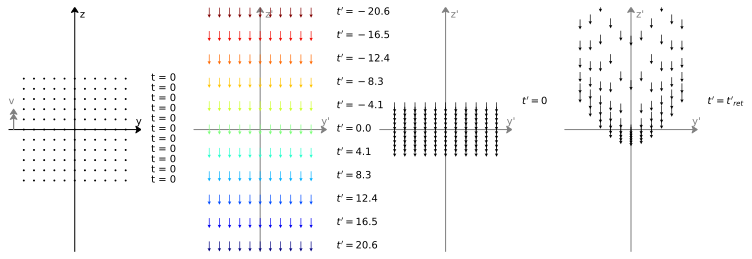
\includegraphics[width=10cm]{images/pdf/coordinate_transforms_2.pdf}

	\caption{A diagram, showing an initial grid of points, representing position coordinates, at time $t=0$ that are at rest in their proper frame ${<\!\!S\!>}$, with an \protect\hyperlink{def-observer}{observer} at the origin (left), giving the direct transformation into the moving primed frame ${<\!\!S{'}\!\!>}$ (second) where the points are now moving at velocity $-v=-0.9$ which is in the negative z-direction with the colors and labels showing the desynchronization of the primed times $t{'}=- {\gamma} \frac{zv}{c^2}$, the next figure (third) shows what these points would be in the same primed frame when they are synchronized with the origin's time $t{'}=0$, the last figure (fourth) shows the same \protect\hyperlink{def-Primed-Frame}{primed frame} ${<\!\!S{'}\!\!>}$ but now with the particles positioned where they would be seen to be at by an \protect\hyperlink{def-observer}{observer} at the origin with the \protect\hyperlink{def-observer}{observer}s time $t{'}=0$, these positions are due to the delay in the light from these particles taking time to get to the \protect\hyperlink{def-observer}{observer}, also known as the \protect\hyperlink{def-retarded-position}{retarded position}s of the particles.}
	\label{fig: full coordinate transform}
\end{figure}
%███████████

*** todo: could include the plot of a larger grid of points to show the distribution of delayed view of particles better, or give the heat map of the density of delayed view coordinates

% %███████████████████████████████████████████████████████████████████
% \subsubsection{Delayed Coordinate Distribution and Density}

% need to find the function for differential dz

% \begin{equation}
% 	\begin{aligned}
% 		 & \frac{dx}{dx{'}} = 1 \\
% 		 & \frac{dy}{dy{'}} = 1 \\
% 		 & \frac{dz}{dz{'}} =
% 	\end{aligned}
% \end{equation}

% *** todo: wanna get the relative delayed view proper coordinate density in the primed frame, there should also be a rotational aspect to it due to the non-uniform distribution of delayed proper coordinates

%███████████████████████████████████████████████████████████████████
%███████████████████████████████████████████████████████████████████
\section{Steps for Changing Frames}

This section outlines the steps that should be taken to change between two inertial frames: \newline

Firstly let us talk about going from the retarded coordinates of objects in one frame to a second frame.
So if in your initial frame, you have an observer at rest at the origin, and different objects are moving around in this frame, if we take the retarded positions $\mathbf{R}_{ret}$ of the objects (i.e.
as the observer sees them positioned due to the delay in the light from the object), and use the retarded times of these objects which is ${t}_{ret}=- \frac{|\mathbf{R}_{ret}|}{c}$ with the coordinate transform, then these retarded positions in the initial reference frame will be transformed to their retarded positions in the second frame at their retarded times within it.
\newline

Another option is that you want to go from the object's positions that have times that are synchronized with the observer to positions that are also synced with the observer in the primed frame.
Then we need to start with all objects where they currently are at $t=0$ then the coordinate transformation transforms the positions to the primed positions in the second frame, but at desynchronized times, so that we will have to propagate these objects forward or back in time until they are all at the time of the observer at the origin which is $t{'}=0$ if the velocities of the objects are constant then you will only need to find their primed velocities, but if the initial frames velocities are not constant this is then a bit trickier, as you will have to worry about the transformations of acceleration to find its position at $t{'}=0$.

%███████████████████████████████████████████████████████████████████
%███████████████████████████████████████████████████████████████████
\section{Variables}

\noindent ${\mathbf{r}}(x,y,z)$ \textbf{:}
...

\noindent ${\mathbf{r}}(r,{\theta},{\phi})$ \textbf{:}
...

\noindent ${dS}$ \textbf{:}
... surface element might be confusing to have as an S due to next chapter

\noindent ${\Omega}$ \textbf{:}
...

\noindent ${d\Omega}$ \textbf{:}
...

\noindent ${\mathbf{c}}(c,\alpha,\varphi)$ \textbf{:}
...

\noindent ${\mathbf{u}}$ \textbf{:}
speed of source which we have chosen to be in z-direction ...

\noindent ${d\lambda}$, ${d\lambda{'}}$ \textbf{:}
...

\noindent ${d\tau}$ \textbf{:}
...

\noindent ${\Phi_{r}}$ \textbf{:}
...

\noindent ${\nu}$, ${\nu{'}}$ \textbf{:}
...

\noindent $T_p,T_{ret}$ \textbf{:}
...

\noindent $L$ \textbf{:}
...

\noindent $\mathbf{s}_{ret}^{'}$ \textbf{:}
...

%███████████████████████████████████████████████████████████████████
%███████████████████████████████████████████████████████████████████
%███████████████████████████████████████████████████████████████████
\chapter{Spherical light pulses}

%███████████████████████████████████████████████████████████████████
%███████████████████████████████████████████████████████████████████
\section{Spherical Polar Coordinates}

This math section is just for reference in later sections,

%█████████████
\begin{figure}[h]
	\figuretitle{...}
	\centering
	\tdplotsetmaincoords{60}{110}
	\tikzsetnextfilename{Tikz_Spherical_Polar_Coordinates}
	\begin{tikzpicture}[scale=3,tdplot_main_coords]
		% variables
		\def\rvec{.8}
		\def\thetavec{30}
		\def\phivec{60}
		% axes
		\coordinate (O) at (0,0,0);
		\draw[thick,->] (O) -- (1,0,0) node[anchor=north east]{$x$};
		\draw[thick,->] (O) -- (0,0.92,0) node[anchor=north west]{$y$};
		\draw[thick,->] (O) -- (0,0,1) node[anchor=south]{$z$};
		% vectors
		\tdplotsetcoord{P}{\rvec}{\thetavec}{\phivec}
		\draw[-stealth,red] (O) -- (P) node[above right] {$\mathbf{R}$};
		\draw[dashed,red] (O) -- (Pxy);
		\draw[dashed,red] (P) -- (Pxy);
		\draw[dashed,red] (Py) -- (Pxy);
		% arcs
		\tdplotdrawarc[->]{(O)}{0.2}{0}{\phivec}
		{anchor=north}{$\phi$}
		\tdplotsetthetaplanecoords{\phivec}
		\tdplotdrawarc[->,tdplot_rotated_coords]{(0,0,0)}{0.5}{0}{\thetavec}
		{anchor=south west}{$\theta$}
		% sphere
		\shadedraw[tdplot_screen_coords,ball color = gray, opacity = 0.3] (0,0) circle (\rvec);
		\draw[fill=gray,opacity=0.3] (0,0) circle (\rvec);
	\end{tikzpicture}
	\caption{Diagram of an axis showing spherical polar coordinates}
\end{figure}
%███████████

For a given coordinate $\mathbf{R}$ we have the Cartesian coordinates $(x,y,z)$, but we can also write this in terms of spherical polar coordinates $(r,\theta,\phi)$ where the angles from the Z-Axis and X-axis respectively are $\theta$ (between 0 and $\pi$) and $\phi$ (between 0 and $2\pi$), and $r$ is the distance to the point from the origin, i.e.
the magnitude $|\mathbf{R}|$.
So that the coordinate can be written as

\begin{equation}
	\mhl{
		\mathbf{R} =
		\begin{pmatrix}
			x \\
			y \\
			z \\
		\end{pmatrix}
		= r
		\begin{pmatrix}
			\cos{\phi}\sin{\theta} \\
			\sin{\phi}\sin{\theta} \\
			\cos{\theta}           \\
		\end{pmatrix}
	}
\end{equation}

with $r=\sqrt{x^2+y^2+z^2}$, $\cos\phi= \frac{x}{\sqrt{x^2+y^2}}$, and $\cos\theta=\frac{z}{r}$.
Some useful formulae for later are the unit vectors

\begin{equation}
	\mathbf{\hat{\text{$r$}}} =
	\begin{pmatrix}
		\sin\theta \, \cos\phi \\
		\sin\theta \, \sin\phi \\
		\cos\theta             \\
	\end{pmatrix},
	\mathbf{\hat{\text{$\theta$}}} =
	\begin{pmatrix}
		\cos\theta \, \cos\phi \\
		\cos\theta \, \sin\phi \\
		- \sin\theta           \\
	\end{pmatrix},
	\mathbf{\hat{\text{$\phi$}}} =
	\begin{pmatrix}
		- \, \sin\phi            \\
		\hphantom{-} \, \cos\phi \\
		0                        \\
	\end{pmatrix}
\end{equation}

and the differentials with respect to each of the coordinates are

\begin{equation}
	\begin{aligned}
		\frac{\partial\mathbf{R}}{\partial r}      & = \mathbf{\hat{\text{$r$}}} \\
		\frac{\partial\mathbf{R}}{\partial \theta} & =
		\begin{pmatrix}
			r \cos\theta \cos\phi \\
			r \cos\theta \sin\phi \\
			-r \sin\theta         \\
		\end{pmatrix}
		=r\mathbf{\hat{\text{$\theta$}}}                                         \\
		\frac{\partial\mathbf{R}}{\partial \phi}   & =
		\begin{pmatrix}
			-r \sin\theta \sin\phi \\
			r \sin\theta \cos\phi  \\
			0
		\end{pmatrix}
		= r \sin\theta \mathbf{\hat{\text{$\phi$}}}
	\end{aligned}
\end{equation}

%███████████████████████████████████████████████████████████████████
%███████████████████████████████████████████████████████████████████
\section{Light Speed Velocity Transform}

The speed of light remains the same after transforming between frames, but the velocity is not as the direction changes.
The velocity transformation in the case where the speed is that of light, $|u|=c$, with the direction in the initial frame at an angle $\alpha$ from the z-axis and $\varphi$ from the x-axis, so that in spherical polar coordinates the velocity of light is

\begin{equation}
	\mathbf{c} = c
	\begin{pmatrix}
		\cos{\varphi}\sin{\alpha} \\
		\sin{\varphi}\sin{\alpha} \\
		\cos{\alpha}              \\
	\end{pmatrix},
\end{equation}

then from the velocity \hyperlink{def-transform}{transform} in eq.
\eqref{eq: velocity transform} we get

% \begin{equation}
% \begin{aligned}
% & {{u}_{x}}^{'} =\frac{c\sin\alpha\cos\varphi}{{\gamma} \bigg(1-\frac{v\cos\alpha}{c}\bigg) } \\ & {{u}_{y}}^{'} =\frac{c\sin\alpha\sin\varphi}{{\gamma} \bigg(1-\frac{v\cos\alpha}{c}\bigg) } \\ & {{u}_{z}}^{'} =\frac{c\cos\alpha -v}{ \bigg(1-\frac{v\cos\alpha}{c}\bigg) }
% \end{aligned}
% \end{equation}

\begin{equation}
	\label{eq: velocity transform for light}
	\mhl{
		\begin{aligned}
			 & \mathbf{c}{'} = \dfrac{c}{{\gamma}\left(1- \frac{v}{c} \cos\alpha\right) }
			\begin{pmatrix}
				\sin\alpha\cos\varphi                            \\
				\sin\alpha\sin\varphi                            \\
				{\gamma} \left( \cos\alpha - \frac{v}{c} \right) \\
			\end{pmatrix}
			\\
			 & \text{at position $\mathbf{R}{'}$ and time $t{'}$ }
		\end{aligned}
	}
\end{equation}

This still has the same speed of light which can be shown by taking the magnitude of the velocity vector (i.e.
the square root of the squares of all its elements).
However, the angle of propagation has been changed.

%███████████████████████████████████████████████████████████████████
%███████████████████████████████████████████████████████████████████
\section{Doppler Effect}

%█████████████
\begin{figure}[H]
	\figuretitle{...}
	\begin{subfigure}{.49\textwidth}
		\centering
		\tikzsetnextfilename{Tikz_Lights_angle_with_particle_in_its_proper_frame}
		\begin{tikzpicture}[scale=8]
			\draw[red,ultra thick, ->] (0,0,0) -- (0.235,-0.05,0) node[midway,anchor= north]{$\mathbf{c}$};
			\fill[black] (0,0,0) circle (0.7pt);
		\end{tikzpicture}
		\caption{Rest Frame}
		% \label{fig:sub2}
	\end{subfigure}
	\begin{subfigure}{.49\textwidth}
		\centering
		\tikzsetnextfilename{Tikz_Lights_angle_with_particle_With_particle_moving}
		\begin{tikzpicture}[scale=8]
			\draw[-] (0,0.07,0) to[bend left=45] (0.06,0.04,0);
			\node at (0.05,0.095,0) {$\alpha{'} $};
			\draw[cyan,ultra thick, ->] (0,0,0) -- (0.21,0.13,0) node[midway,anchor= north]{$\mathbf{c}{'}$};
			\draw[ultra thick, ->] (0,0,0) -- (0,0.15,0)node[midway,anchor=east]{$\mathbf{u}_s^{'}$};
			\fill[black] (0,0,0) circle (0.7pt);
		\end{tikzpicture}
		\caption{Moving Frame}
		% \label{fig:sub1}
	\end{subfigure}
	\caption{Diagrams of Light being emitted by a source in two different frames.}
	\label{fig: Doppler effect}
\end{figure}
%███████████

In the rest frame of a source $s$, if it emits a wave at the speed of light in any direction, we have the length the wave has traveled from the source in the time $d\tau$ as being
\begin{equation}
	d\lambda = cd\tau
\end{equation}
If we change to a frame where the source is now moving at speed $u_s^{'}$ in the z-direction and we have the wave now emitted at an angle $\alpha{'}$ from the z-axis, traveling distance $cdt{'}$ in a time $dt{'}$, with the particle moving a distance $ u_s^{'} \cos\alpha{'} dt{'}$ in the direction of this emitted part of the wave, this leads to a bunching up of the wave in the direction of the movement of the particle, as the same amount of the wave has been emitted in this primed time, but the distance it has traveled from source is

\begin{equation}
	d\lambda{'} = cdt{'} - u_{s}^{'} \cos\alpha{'} dt{'}= (1-\frac{u_{s}^{'}}{c}\cos\alpha{'})cdt{'}
\end{equation}

we have $dt{'}={\gamma} d\tau$, so the ratio of space the wave takes up in that direction compared to in the \hyperlink{def-proper-frame}{rest frame} is

\begin{equation}
	Ratio = \frac{d\lambda'}{d\lambda} = {\gamma} \left(1-\dfrac{u_{s}^{'}}{c} \cos\alpha{'} \right)
\end{equation}

since wavelength is inversely proportional to the frequency, and this bunching up at the front will proportionally decrease the wavelength

\begin{equation}
	\Phi_{r} = \frac{1}{ {\gamma} \left(1-\dfrac{u_{s}^{'}}{c} \cos\alpha{'} \right)}
\end{equation}

%███████████████████████████████████████████████████████████████████
%███████████████████████████████████████████████████████████████████
\section{Aberration in Special Relativity}

%█████████████
\begin{figure}[ht]
	\figuretitle{...}
	\begin{subfigure}{.49\textwidth}
		\centering
		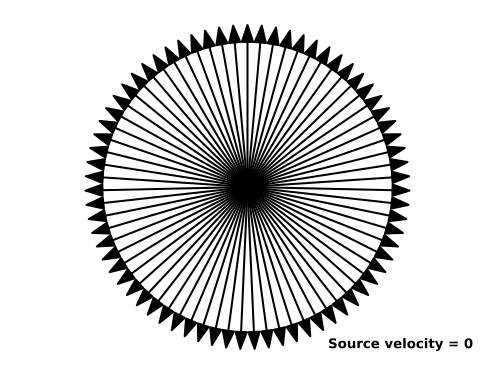
\includegraphics[width=5cm]{images/pdf/Aberrated_velocities_restframe.pdf}
		\caption{rest frame}
	\end{subfigure}
	\begin{subfigure}{.49\textwidth}
		\centering
		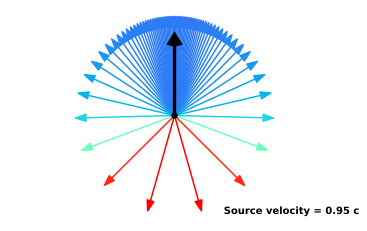
\includegraphics[width=5cm]{images/pdf/Aberrated_velocities.pdf}
		\caption{moving frame}
	\end{subfigure}
	\caption{Diagram showing the directions of propagation of an evenly distributed light pulse in the rest frame of a source and the corresponding distribution in a frame in which the source is now moving, with the colors showing the Doppler effect on the light's frequency.}
	\label{fig: aberrated emitted light}
\end{figure}
%███████████

The propagation directions of the light as seen in Figure (\ref{fig: aberrated emitted light}), are transformed such that the angles between them and the Z-Axis, have the aberrational relationship

\begin{equation}
	\label{eq: Cosine transform}
	\mhl{
		\cos\alpha{'} = \frac{\mathbf{c}_{z}^{'}}{\|\mathbf{c}{'}\|} = \dfrac{\cos\alpha + \dfrac{u_{s}^{'}}{c}}{1+\dfrac{u_{s}^{'}}{c}\cos\alpha}.
	}
\end{equation}

This is the relativistic aberration formula \cite{einstein1905electrodynamics}, it shows how the field's propagation direction transforms.
Figure (\ref{fig: aberrated absorbed light}) shows what would happen in the case of incoming light from all directions.

%█████████████
\begin{figure}[ht]
	\figuretitle{...}
	\begin{subfigure}{.49\textwidth}
		\centering
		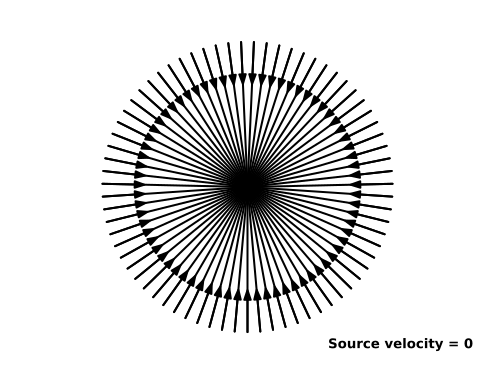
\includegraphics[width=5cm]{images/pdf/Aberrated_velocities_inwards_restframe.pdf}
		\caption{rest frame}
	\end{subfigure}
	\begin{subfigure}{.49\textwidth}
		\centering
		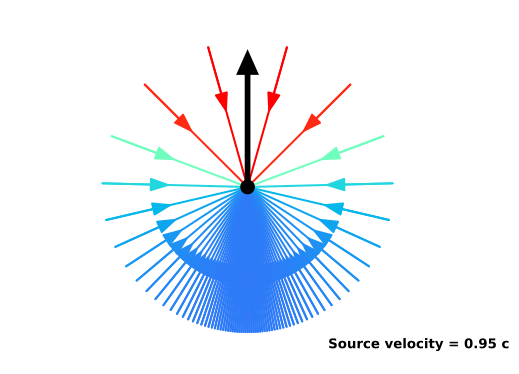
\includegraphics[width=5cm]{images/pdf/Aberrated_velocities_inwards.pdf}
		\caption{moving frame}
	\end{subfigure}
	\caption{Diagram showing the directions of evenly distributed light being absorbed by a particle in its rest frame and the corresponding distribution in a frame in which the particle is now moving, with the colors showing the Doppler effect on the light's frequency.}
	\label{fig: aberrated absorbed light}
\end{figure}
%███████████

It can be seen from eq.
\eqref{eq: Cosine transform} that as a source's speed tends to the speed of light, $\cos\alpha{'}$ tends to $1$ as the top and bottom of the fraction cancel each other out, hence all emitted or absorbed light in the source's rest frame tends to the direction of the source's movement.
But we also have to remember that if there was any time between the start and finishing of the emitting the light, this time would tend to infinity as well, basically any emitted light would remain in the vicinity of the source.

%███████████████████████████████████████████████████████████████████
%███████████████████████████████████████████████████████████████████
\section{Transform of Light Pulse from Origin}

%█████████████
\begin{figure}[H]
	\figuretitle{...}
	\begin{subfigure}{.49\textwidth}
		\tikzsetnextfilename{Tikz_Light_Pulse_Proper_Frame}
		\begin{tikzpicture}[scale=4.9] %[,tdplot_main_coords]
			%\usetikzlibrary{arrows.meta}
			\node[blue] at (0.06,-0.06,0) {$\mathbf{s}$};
			\draw[blue, thick,->] (0,0,0) -- (0.4,0,0) node[anchor=north east]{$y$};
			\draw[blue, thick,->] (0,0,0) -- (0,0.4,0) node[anchor=north west]{$z$};
			\draw[blue, thick,->] (0,0,0) -- (0,0,0.55) node[anchor=south east] {$x$};
			\node[red] at (0.08,0.17,0) {$\alpha $};
			\draw[red,->] (0,0.25,0) to[bend left=45] (0.21,0.145,0);
			\draw[thick,red, dotted,->] (0,0,0) -- (0.69,0.46,0) node[midway , right] {\text{ $\mathbf{c} {T}_{p}$}};
			\fill[blue] (0,0,0) circle (1pt);
			\fill[black] (0.71,0.48,0) circle (0.4pt) node[above] {\text{$ \mathbf{R}$}};
		\end{tikzpicture}
		\caption{\hyperlink{def-proper-frame}{proper frame}}
		\label{fig: proper frame 1}
	\end{subfigure}
	\begin{subfigure}{.49\textwidth}
		\tikzsetnextfilename{Tikz_Light_Pulse_Primed_Frame}
		\begin{tikzpicture}[scale=4.9] %[,tdplot_main_coords]
			%\usetikzlibrary{arrows.meta}
			%node[anchor = north west]{\textcolor{black}{ $\mathbf{P}{'}$}}; %$\mathbf{P}{'}$}};
			\node[gray] at (0.1,-0.1,0) {$\mathbf{s}_{ret}^{'}$};
			\draw[gray!40,fill=gray!40] (0,0,0) circle (1pt);
			\draw[black, thick,->] (0,0.7,0) -- (0.29,0.7,0) node[anchor=north]{{\color{blue} $y$},$y{'}$};
			\draw[black, thick,->] (0,0.7,0) -- (0,1,0) node[anchor=west]{{\color{blue} $z$},$z{'}$};
			\draw[black, thick,->] (0,0.7,0) -- (0,0.7,0.45) node[anchor=south east] {{\color{blue} $x$}, $x{'}$};
			\draw[gray, dashed,->] (0,0,0) -- (0.25,0,0) node[anchor=south east]{$y$};
			\draw[gray, dashed,->] (0,0,0) -- (0,0.2,0) node[anchor=north east]{$z$};
			\draw[gray, dashed,->] (0,0,0) -- (0,0,0.35) node[anchor=south east] {$x$};
			\node[red] at (0.06,0.17,0) {$\alpha {'}$};
			\draw[red,->] (0,0.25,0) to[bend left=40] (0.15,0.2,0);
			\draw[red, thick, dotted,->] (0,0,0) -- (0.69*0.85,0.88*0.85,0) node[midway, right] {$\mathbf{c}{'} {T}_{p}^{'}$};
			\draw[gray, thick, dotted] (0.69*0.85,0.88*0.85,0) -- (0.69,0.88,0);
			\draw[black,->] (0,0.7,0) -- (0.68,0.9,0) node[midway,above] {\text{ $\mathbf{R}{'}$}};
			\draw[black,->] (0,0.7,0) -- (0.68*0.85,0.9*0.85,0);
			\node at (0.4,0.68,0) {\text{ $\mathbf{L}{'}$}};
			\draw[blue, fill=blue] (0,0.7,0) circle (1pt) node[anchor=north west]{$\mathbf{s}{'}$};
			\draw[thick,blue,dotted,->] (0,0,0) -- (0,0.66,0);
			\draw[blue, thick,->>] (0,0.7,0) -- (0,0.8,0) node[left]{$\mathbf{u}_s$};
			\fill (0.7,0.9,0) circle (0.4pt);
			\node[blue, right] at (0,0.4,0) {$\mathbf{u}_s {T}_{p}^{'}$};
		\end{tikzpicture}
		\caption{\hyperlink{def-Primed-Frame}{primed frame} with moving source}
		\label{fig: primed frame 1}
	\end{subfigure}
	\caption{The diagram shows a source particle $s$ in blue at rest in the \protect\hyperlink{def-proper-frame}{proper frame}, Fig (a), with a light pulse that has propagated along $\mathbf{c} {T}_{p}$ shown in red, at an angle $\alpha$ from the z-axis, to coordinate $\mathbf{R}$ shown in black, with the current time for whole system being $t=0$. Fig (b), shows the system transformed to a \protect\hyperlink{def-Primed-Frame}{primed frame} moving at velocity $\mathbf{v}=(0,0,v)$ in the z-direction relative to the \protect\hyperlink{def-proper-frame}{proper frame}, such that the particle and its attached proper axis in this frame are moving at velocity $\mathbf{u}_s= - \mathbf{v}$ and is currently at the primed origin with time $t{'}=0$. when the light was emitted from the particle, the particle and attached proper axis were at the \protect\hyperlink{def-retarded-position}{retarded position} $\mathbf{s}_{ret}^{'}$ shown in grey, the emitted light was then propagated at an angle $\alpha{'}$ from the z-axis, along $\mathbf{c}{'} {T}_{p}^{'}$ to reach $\mathbf{L}{'}$ at $t{'}=0$. it has not yet reached the corresponding \protect\hyperlink{def-lorentz-transform}{Lorentz transformed} coordinate $\mathbf{R}{'}$.}
	\label{fig: Retarded field outward field transform}
\end{figure}
%███████████

As visualized in figure (\ref{fig: Retarded field outward field transform}).
If we have a light source particle $s$, in its \hyperlink{def-proper-frame}{rest frame} that had emitted a pulse of light in one direction such that it propagates along $\mathbf{c} {T}_{p}$ at an angle $\alpha$ from the z-axis and is currently at position $\mathbf{R}$ at time $t=0$, where $\mathbf{c}$ is the velocity of light and ${T}_{p}$ is the time it took to propagate to $\mathbf{R}$.
Using the coordinated transform from eq.
\eqref{eq: Lorentz transformation} on $\mathbf{R}$ with $t=0$ we get

\begin{equation}
	\label{eq: displacement transform}
	\begin{aligned}
		\mathbf{R}{'} & =
		\begin{pmatrix}
			x          \\
			y          \\
			{\gamma} z \\
		\end{pmatrix},                            \\
		\text{at time \ \ \ }                     \\
		t{'}          & = - {\gamma} \frac{vz}{c^2} \\
	\end{aligned}
\end{equation}

the light pulse's velocity using the velocity transform from eq.
\eqref{eq: velocity transform for light} in Cartesian coordinates and particles speed in the \hyperlink{def-Primed-Frame}{primed frame} with $v=-u_s$ is

\begin{equation}
	\label{eq: light pulse velocity transform}
	\mathbf{c}{'} = \dfrac{c}{{\gamma}\left(1 + \frac{z}{\|\mathbf{R}\|} \dfrac{u_s}{c} \right)}
	\begin{pmatrix}
		\frac{x}{\|\mathbf{R}\|}                                          \\
		\frac{y}{\|\mathbf{R}\|}                                          \\
		{\gamma} \left( \frac{z}{\|\mathbf{R}\|} + \dfrac{u_s}{c} \right) \\
	\end{pmatrix}
\end{equation}

% can also show in spherical polar coordinates

The time that the particle emits the light in the \hyperlink{def-proper-frame}{proper frame} is ${T}_{ret}= - {T}_{p}$ which corresponds to the contracted time

\begin{equation}
	t{'}_{ret}= {\gamma} {T}_{ret} = - {\gamma} {T}_{p}
\end{equation}

So that in the \hyperlink{def-Primed-Frame}{primed frame}, the \hyperlink{def-retarded-position}{retarded position} of the source particle emits the light pulse is

\begin{equation}
	\mathbf{s}_{ret}^{'} = - {\gamma} {T}_{p} \mathbf{u}_s
\end{equation}

to find the position the light pulse is currently at, at time $t{'}=0$, we have to rewind its time from the position $\mathbf{R}{'}$ that it is at when using the \hyperlink{def-lorentz-transform}{Lorentz transform} at time $t{'}= -{\gamma}\frac{vz}{c^2}= {\gamma}\frac{u_s z}{c^2}$ taking away the displacement it propagated in this time to get the current position of the light to be ($t{'}_{p}=- t{'}_{ret}$).

\begin{equation}
	\begin{split}
		\mathbf{L}{'}
		 & = \mathbf{s}_{ret}^{'} + \mathbf{c}{'}t{'}_{p}
		\\
		 & = \left( \mathbf{c}{'} - \mathbf{u}_s \right)t{'}_{p}
		\\
		 & = \dfrac{c t{'}_{p}}{{\gamma}\left(1 + \frac{z}{\|\mathbf{R}\|} \dfrac{u_s}{c} \right)}
		\begin{pmatrix}
			\frac{x}{\|\mathbf{R}\|}                                          \\
			\frac{y}{\|\mathbf{R}\|}                                          \\
			{\gamma} \left( \frac{z}{\|\mathbf{R}\|} + \dfrac{u_s}{c} \right) \\
		\end{pmatrix}
		-
		\begin{pmatrix}
			0          \\
			0          \\
			u_s t{'}_{p} \\
		\end{pmatrix}
		\\
		 & = \dfrac{c t{'}_{p}}{{\gamma}\left(1 + \frac{z}{\|\mathbf{R}\|} \dfrac{u_s}{c} \right)}
		\begin{pmatrix}
			\frac{x}{\|\mathbf{R}\|}                                                                                                                             \\
			\frac{y}{\|\mathbf{R}\|}                                                                                                                             \\
			{\gamma} \left( \frac{z}{\|\mathbf{R}\|} + \dfrac{u_s}{c} \right) - {\gamma}\left(1 + \frac{z}{\|\mathbf{R}\|} \dfrac{u_s}{c} \right) \dfrac{u_s}{c} \\
		\end{pmatrix}
	\end{split}
\end{equation}
which leads to
\begin{equation}
	\mathbf{L}{'} = \dfrac{c t{'}_{p}}{{\gamma}\left(1 + \frac{z}{\|\mathbf{R}\|} \dfrac{u_s}{c} \right)}
	\begin{pmatrix}
		\frac{x}{\|\mathbf{R}\|}                    \\
		\frac{y}{\|\mathbf{R}\|}                    \\
		\frac{1}{{\gamma}} \frac{z}{\|\mathbf{R}\|} \\
	\end{pmatrix}
\end{equation}

%███████████████████████████████████████████████████████████████████
%███████████████████████████████████████████████████████████████████
\section{Relativistic Beaming}

The previous section can be used to show us what happens to the angles of propagation in a spherical pulse of light with evenly distributed angles.
Substituting $\frac{x}{\|\mathbf{R}\|}= \cos{\varphi}\sin{\alpha}$, $\frac{y}{\|\mathbf{R}\|} = \sin{\varphi}\sin{\alpha}$ and $ \frac{z}{\|\mathbf{R}\|} = \cos{\alpha}$ for spherical polar coordinates, which leads to

%█████████████
\begin{figure}[H]
	\figuretitle{...}
	\begin{subfigure}{.32\textwidth}
		\centering
		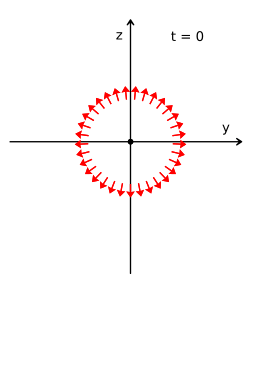
\includegraphics[width=3.8cm]{images/pdf/Rest_Pulse.pdf}
		\caption{Source's Rest Frame}
	\end{subfigure}
	\begin{subfigure}{.32\textwidth}
		\centering
		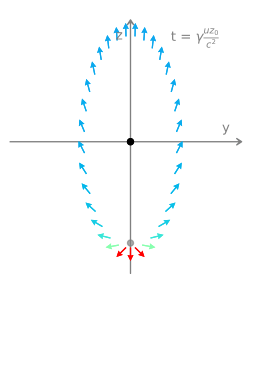
\includegraphics[width=3.8cm]{images/pdf/Prime_Pulse.pdf}
		\caption{Source's Moving frame}
	\end{subfigure}
	\begin{subfigure}{.32\textwidth}
		\centering
		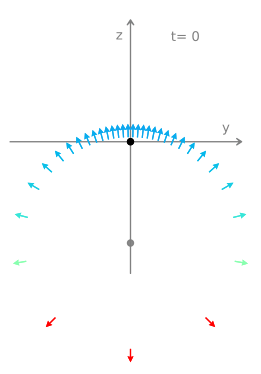
\includegraphics[width=3.8cm]{images/pdf/Prime_Pulse_Simultaneous.pdf}
		\caption{Source's Moving frame}
	\end{subfigure}
	\caption{Diagram showing, the position of light pulse after a certain amount of time, first in the rest frame and next in the primed frame, the direct coordinate transform gives the ellipsoid with coordinates having different times, and the circular pulse in the primed frame is when you account for this and propagate each part of the pulse, to back or forward in time so that each part has the same time as the origin. *** could have the proper axis with different colors}
	%\label{fig: truck aberrated}
\end{figure}
%███████████

If we then did the same for multiple pulses to see how they \hyperlink{def-transform}{transform}, noting that the time between each pulse is the dilated time in the primed frame.

%█████████████
\begin{figure}[H]
	\figuretitle{...}
	\begin{subfigure}{.49\textwidth}
		\centering
		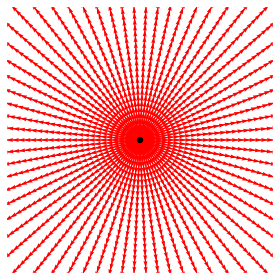
\includegraphics[width=5cm]{images/pdf/Field_Rest_Frame.pdf}
		\caption{Source's Rest Frame}
	\end{subfigure}
	\begin{subfigure}{.49\textwidth}
		\centering
		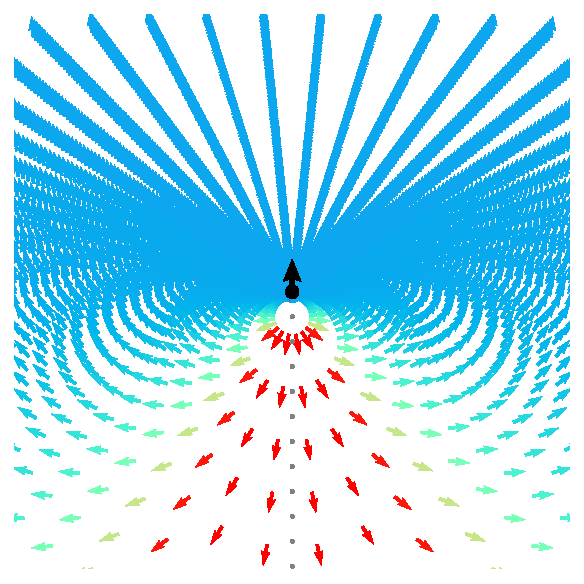
\includegraphics[width=5cm]{images/pdf/Field_Moving_Frame_Doppler.pdf}
		\caption{Source's Moving frame}
	\end{subfigure}
	\caption{A 2D diagram showing multiple spherically symmetrical pulses of light from a source at rest (left), and in a corresponding primed inertial frame where the source is moving (right), the colors show the \protect\hyperlink{def-doppler-effect}{Doppler effect} on lights light *** describe it as spherical waves with them being closer together in the direction of movement, could have separate diagram showing the concentric circles with different origins}
	\label{fig: full field transformation}
\end{figure}
%███████████

%███████████████████████████████████████████████████████████████████
%███████████████████████████████████████████████████████████████████
\section{Variables}

\noindent ${\Delta S}$ \textbf{:}
...

\noindent ${\Delta S_p}$ \textbf{:}
... $({\delta x_p},{\delta y_p},{\delta z_p},{\delta t_p})$

\noindent ${m}$ \textbf{:}
...

\noindent ${\gamma_u}$ \textbf{:}
...

\noindent ${\delta \tau}$ \textbf{:}
...

\noindent ${E}$ \textbf{:}
...

\noindent ${E_0}$ \textbf{:}
...

\noindent ${p}$ \textbf{:}
... momentum


%███████████████████████████████████████████████████████████████████
%███████████████████████████████████████████████████████████████████
%███████████████████████████████████████████████████████████████████
\chapter{A Moving Source's Field}

%█████████████
\begin{figure}[H]
	\figuretitle{...}
	\begin{subfigure}{.49\textwidth}
		\centering
		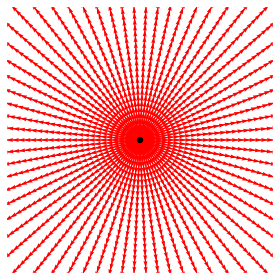
\includegraphics[width=5cm]{images/pdf/Field_Rest_Frame.pdf}
		\caption{Source's Rest Frame}
	\end{subfigure}
	\begin{subfigure}{.49\textwidth}
		\centering
		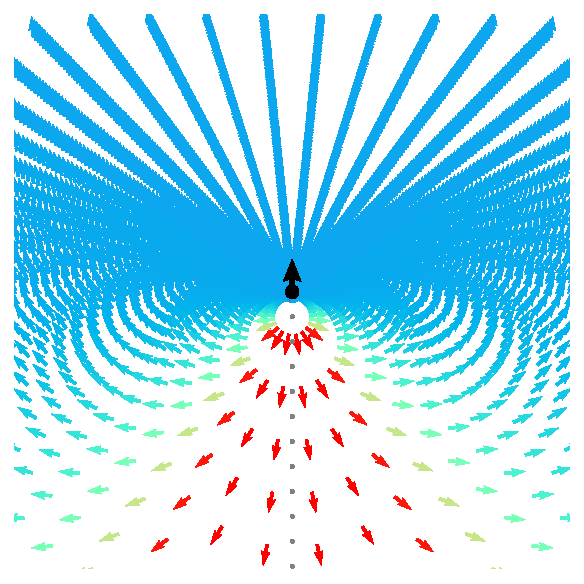
\includegraphics[width=5cm]{images/pdf/Field_Moving_Frame_Doppler.pdf}
		\caption{Source's Moving frame}
	\end{subfigure}
	\caption{A 2D diagram showing multiple spherically symmetrical pulses of light from a source at rest (left), and in a corresponding primed inertial frame where the source is moving (right), the colors show the \protect\hyperlink{def-doppler-effect}{Doppler effect} on lights light *** describe it as spherical waves with them being closer together in the direction of movement, could have separate diagram showing the concentric circles with different origins}
	\label{fig: full field transformation 2}
\end{figure}
%███████████

*** What is the change in the rate of change of direction at a coordinate of the light $\frac{d\alpha(y{'},z{'},t{'})}{dt{'}}$ (maybe try $\frac{d\cos\alpha(y{'},z{'},t{'})}{dt{'}}$ and $\frac{d\sin\alpha(y{'},z{'},t{'})}{dt{'}}$ instead) and find at $t{'}=0$ what is the change in the angle with change in position $\frac{d\alpha(y{'},z{'},t{'})}{dy{'}}$, $\frac{d\alpha(y{'},z{'},t{'})}{dz{'}}$ and $\frac{d^2\alpha(y{'},z{'},t{'})}{dy{'}dz{'}}$

*** What is the density of the field at a certain point, using $k \frac{1}{R^2}$ in a proper frame, and then taking into account the distance from coordinate to retarded position of the source and then the aberration and Doppler effect

%███████████████████████████████████████████████████████████████████
%███████████████████████████████████████████████████████████████████
\section{Flux from Point Source}

- flux describes the rate at which a quantity flows across a surface (flowrate per unit area)

%███████████████████████████████████████████████████████████████████
\subsection{Surface element}

%█████████████
\begin{figure}[h]
	\figuretitle{Differential Element in Spherical Polar Coordinates}
	\centering
	\tikzsetnextfilename{Tikz_Surface_Element}
	%Axis Angles
	\tdplotsetmaincoords{70}{110}
	%
	%Macros
	\pgfmathsetmacro{\rvec}{6}
	\pgfmathsetmacro{\thetavec}{40}
	\pgfmathsetmacro{\phivec}{45}
	\pgfmathsetmacro{\dphivec}{20}
	\pgfmathsetmacro{\dthetavec}{20}
	\pgfmathsetmacro{\drvec}{1.5}
	%
	%Layers
	\pgfdeclarelayer{background}
	\pgfdeclarelayer{foreground}
	%
	\pgfsetlayers{background, main, foreground}
	\scalebox{0.8}{
		\begin{tikzpicture}[tdplot_main_coords]
			\shadedraw[tdplot_screen_coords,ball color = gray, opacity = 0.3] (0,0) circle (\rvec);
			\draw[fill=gray,opacity=0.3] (0,0) circle (\rvec);
			%
			%Coordinates
			\coordinate (O) at (0,0,0);
			\tdplotsetcoord{A}{\rvec}{\thetavec}{\phivec}
			\tdplotsetcoord{B}{\rvec}{\thetavec + \dthetavec}{\phivec}
			\tdplotsetcoord{C}{\rvec}{\thetavec + \dthetavec}{\phivec + \dphivec}
			\tdplotsetcoord{D}{\rvec}{\thetavec}{\phivec + \dphivec}
			\tdplotsetcoord{E}{\rvec + \drvec}{\thetavec}{\phivec}
			\tdplotsetcoord{F}{\rvec + \drvec}{\thetavec + \dthetavec}{\phivec}
			\tdplotsetcoord{F'}{\rvec + \drvec}{90}{\phivec}
			\tdplotsetcoord{G}{\rvec + \drvec}{\thetavec + \dthetavec}{\phivec + \dphivec}
			\tdplotsetcoord{G'}{\rvec + \drvec}{90}{\phivec + \dphivec}
			\tdplotsetcoord{H}{\rvec + \drvec}{\thetavec}{\phivec + \dphivec}
			%
			%Axis
			\begin{pgfonlayer}{background}
				\draw[thick,-latex] (0,0,0) -- (7,0,0) node[pos=1.1]{$x$};
				\draw[thick,-latex] (0,0,0) -- (0,6.8,0) node[anchor = south east]{$y$};
				\draw[thick,-latex] (0,0,0) -- (0,0,5.5) node[pos=1.05]{$z$};
			\end{pgfonlayer}
			%
			%Help Lines
			\begin{pgfonlayer}{background}
				%Up
				\draw[thick, blue] (O) -- (A) node[pos=0.6, above left, blue] {$r$};
				\draw (O) -- (B);
				\draw (O) -- (C);
				\draw[dashed] (O) -- (D);
				%Down
				\draw (O) -- (F');
				\draw (O) -- (G');
			\end{pgfonlayer}
			\begin{pgfonlayer}{foreground}
				%%Help Curves
				\tdplotsetthetaplanecoords{\phivec}
				\tdplotdrawarc[tdplot_rotated_coords]{(O)}{\rvec}{\thetavec+\dthetavec}{90}{}{}
				%
				\tdplotdrawarc[tdplot_rotated_coords]{(O)}{\rvec+\drvec}{\thetavec+\dthetavec}{90}{}{}
				%
				\tdplotsetthetaplanecoords{\phivec+\dphivec}
				\tdplotdrawarc[tdplot_rotated_coords, dashed]{(O)}{\rvec}{\thetavec+\dthetavec}{90}{}{}
				\tdplotdrawarc[tdplot_rotated_coords]{(O)}{\rvec+\drvec}{\thetavec+\dthetavec}{90}{}{}
				%
				\tdplotdrawarc[tdplot_main_coords]{(O)}{\rvec}{\phivec}{\phivec+\dphivec}{}{}
				%
				\tdplotdrawarc[tdplot_main_coords]{(O)}{\rvec+\drvec}{\phivec}{\phivec+\dphivec}{below, rotate=13}{$r\sin\theta\mathrm{d}\phi$}
			\end{pgfonlayer}
			%
			%Angles
			\begin{pgfonlayer}{foreground}
				%Phi
				\tdplotdrawarc[-stealth]{(O)}{0.9}{0}{\phivec}{anchor=north}{$\phi$}
				\tdplotdrawarc[-stealth]{(O)}{1.5}{\phivec}{\phivec + \dphivec}{}{}
				\node at (1.4,1.9,0) {$\mathrm{d}\phi$};
				\tdplotsetthetaplanecoords{\phivec}
				%Theta
				\tdplotdrawarc[tdplot_rotated_coords,-stealth]{(0,0,0)}{1.2}{0}{\thetavec}{}{}
				\node at (0,0.3,1.3) {$\theta$};
				\tdplotdrawarc[tdplot_rotated_coords,-stealth]{(0,0,0)}{2.5}{\thetavec}{\thetavec + \dthetavec}{anchor=south west}{$\mathrm{d}\theta$}
			\end{pgfonlayer}
			%
			%Differential Volume
			%
			%%Lines
			\begin{pgfonlayer}{foreground}
				\draw[thick] (A) -- (E) node[midway, above left]{$\mathrm{d}r$};
				\draw[thick] (B) -- (F);
				\draw[thick] (C) -- (G);
			\end{pgfonlayer}
			\begin{pgfonlayer}{background}
				\draw[dashed, thick] (D) -- (H);
			\end{pgfonlayer}
			%
			%%Curved
			\begin{pgfonlayer}{background}
				\tdplotsetrotatedcoords{55}{-50.4313}{-6.4086}
				\tdplotdrawarc[dashed, tdplot_rotated_coords, thick]{(O)}{\rvec}{0}{12.8173}{}{}
				%
				\tdplotsetthetaplanecoords{\phivec + \dphivec}
				\tdplotdrawarc[dashed, tdplot_rotated_coords, thick]{(O)}{\rvec}{\thetavec}{\dthetavec + \thetavec}{}{}
			\end{pgfonlayer}
			\begin{pgfonlayer}{foreground}
				\tdplotsetthetaplanecoords{\phivec}
				\tdplotdrawarc[tdplot_rotated_coords, thick]{(O)}{\rvec}{\thetavec}{\dthetavec + \thetavec}{}{}
				\tdplotdrawarc[tdplot_rotated_coords, thick]{(O)}{\rvec + \drvec}{\thetavec}{\dthetavec + \thetavec}{}{}
				%
				\tdplotsetthetaplanecoords{\phivec + \dphivec}
				\tdplotdrawarc[tdplot_rotated_coords, thick]{(O)}{\rvec + \drvec}{\thetavec}{\dthetavec + \thetavec}{above right}{$r\mathrm{d}\theta$}
				%
				\tdplotsetrotatedcoords{55}{-50.4313}{-6.4086}
				\tdplotdrawarc[tdplot_rotated_coords, thick]{(O)}{\rvec + \drvec}{0}{12.8173}{}{}
				%
				\tdplotsetrotatedcoords{55}{-30.3813}{-8.6492} %
				\tdplotdrawarc[tdplot_rotated_coords, thick]{(O)}{\rvec}{0}{17.2983}{}{}
				\tdplotdrawarc[tdplot_rotated_coords, thick]{(O)}{\rvec + \drvec}{0}{17.2983}{}{}
			\end{pgfonlayer}
			%
			%Fill Color
			\begin{pgfonlayer}{main}
				%Front
				\fill[black, opacity=0.15] (E) to (A) to[bend left=4] (B) to (F) to[bend right=4] cycle;
				\fill[black, opacity=0.6] (E) to[bend left=4] (F) to[bend left=2] (G) to[bend right=6.5] (H) to[bend right=4] cycle;
				\fill[black, opacity=0.4] (F) to[bend left=2] (G) to[bend left=1.5] (C) to[bend right=2.5] (B) to[bend right=4] cycle;
			\end{pgfonlayer}
			\begin{pgfonlayer}{background}
				%Back
				\fill[black!50, opacity=0.5] (A) to[bend left=2] (D) to[bend left=6] (C) to[bend right=2.5] (B) to[bend right=4] cycle;
				\fill[black!50, opacity=0.5] (A) to[bend left=2] (D) to (H) to[bend right=2.5] (E) to[bend right=4] cycle;
				\fill[black!50, opacity=0.5] (D) to (H) to[bend left=6] (G) to[bend right=2] (C) to[bend right=6] cycle;
			\end{pgfonlayer}
		\end{tikzpicture}
	}
	\caption{...}
\end{figure}
%███████████

The surface element spanning from $\theta$ to $\theta + d\theta$ and $\phi$ to $\phi + d\phi$ on a spherical surface at (constant) radius r is then

\begin{equation}
	\mathrm{d}S =
	\left\|\frac{\partial {\mathbf R}}{\partial \theta} \times \frac{\partial {\mathbf R}}{\partial \phi}\right\| \mathrm{d}\theta \,\mathrm{d}\phi = \left| r \mathbf{\mathbf{\hat{\text{$\theta$}}}} \times r \sin \theta \mathbf{\mathbf{\hat{\text{$\phi$}}}} \right|= r^2 \sin\theta \,\mathrm{d}\theta \,\mathrm{d}\phi
\end{equation}

The differential solid angle is

\begin{equation}
	\mathrm{d}\Omega = \frac{\mathrm{d}S}{r^2} = \sin\theta \,\mathrm{d}\theta \,\mathrm{d}\phi
\end{equation}%██████

A solid angle $\Omega$ is a measure of the amount of the field of view from some particular point that a given object covers.
The fraction of the field of view covered from a point is given by $\Omega/ 4\pi$

%███████████████████████████████████████████████████████████████████
\subsection{Field Flux}

A \hyperlink{def-proper-frame}{proper frame} of a particle's differential solid angle element (definition given in previous chapter (maybe move that subsection to here))

\begin{equation}
	d\Omega = \sin{\theta} d\theta d\phi,
\end{equation}

encompasses a certain amount of the wavefront, this is the same amount of the wavefront that is encompassed by the coinciding aberrated differential solid angle

\begin{equation}
	d\Omega{'} = \sin{\theta'} d\theta{'} d\phi{'}.
\end{equation}

We can calculate this element by differentiating both sides of eq.
\eqref{eq: Cosine transform} with respect to $\theta$ \cite{hogg1997special}, which gives

\begin{equation}
	\sin{\theta'} d\theta{'} = \dfrac{1-\dfrac{u_s^2}{c^2}}{\left(1+\dfrac{u_s}{c}\cos{\theta}\right)^2} \sin{\theta} d\theta = \dfrac{1}{{\gamma}^2\left(1+\dfrac{u_s}{c}\cos{\theta}\right)^2} \sin{\theta} d\theta
\end{equation}

as $v=-u_s$ now using this and $d\phi{'}=d\phi$ (as the angle $\phi$ is always perpendicular to the motion of the particle and hence unaffected by \hyperlink{def-transform}{transformation} ) we have the solid angle in the \hyperlink{def-Primed-Frame}{primed frame} given as

\begin{equation}
	\mhl{
		d\Omega{'} = \dfrac{1}{{\gamma}^2\left(1+\dfrac{u_s}{c}\cos{\theta}\right)^2} \sin{\theta} d\theta d\phi.
	}
\end{equation}

%The overall amount of wavefront is conserved, as can be seen when integrating over the corresponding solid angle in either frame, both of which give the same value of $4\pi$.
% proportional to the amount of the wavefront in the given proper differential element of the solid angle, and
The relative primed wavefront strength at a given angle is taken as being proportional to the amount of the wavefront per solid angle in the \hyperlink{def-Primed-Frame}{primed frame} relative to that in the \hyperlink{def-proper-frame}{proper frame}, referred to here as the aberrational wavefront strength weighting, given as

\begin{equation}
	\label{eq: aberrational wavefront weighting}
	\Phi_\Omega = \frac{d\Omega}{d\Omega'} = \text{\AA}^2.
\end{equation}

(define what I mean by strength weighting)

*** This flux does not take into account that the source keeps changing position, so at a change ds from position field is coming from a different retarded position of the source, so there is a rotation of direction and a different flux, there is gradients and rotations

*** This flux transform is the change in flux in the emitted direction from the source only not what another particle would feel

%███████████████████████████████████████████████████████████████████
%███████████████████████████████████████████████████████████████████
\section{Variables}

\variable{${\Delta S}$}{
...
}

\variable{${\Delta S_p}$}{
... $({\delta x_p},{\delta y_p},{\delta z_p},{\delta t_p})$
}

\variable{${m}$}{
...
}

\variable{${\gamma_u}$}{
...
}

\variable{${\delta \tau}$}{
...
}

\variable{${E}$}{
...
}

\variable{${E_0}$}{
...
}

\variable{${p}$}{
... momentum
}


%███████████████████████████████████████████████████████████████████
%███████████████████████████████████████████████████████████████████
%███████████████████████████████████████████████████████████████████
\chapter{Invariant Quantities}

Quantities that are frame-independent, i.e.
do not change when we transform between inertial reference frames, are called \hyperlink{def-lorentz-invariant}{Lorentz invariant}.

In this chapter, we will see the invariant quantity related to space-time coordinates and use this to find invariant properties associated with velocity, which will lead to the more abstract conservation relation of momentum energy and mass.
We will find a new quantity with the units of energy that has a term which approximates to the kinetic energy of a particle at low velocities and another term that suggests particles have a new type of energy, that was not previously in classical physics, that depends on the mass of a particle (mass-energy equivalence), this will all lead to a new conservation law of energy.
 The reason we care about the concept of energy is that it has a conservation relation that can be used as a tool to help us make calculations and model more complex systems.

%███████████████████████████████████████████████████████████████████
%███████████████████████████████████████████████████████████████████
\section{Space-Time Interval}

*** maybe explain the interval on a complex triangle instead with it being the hypotenuse and sides being cti and r

We define a quantity called the space-time interval $\Delta S$ between two \hyperlink{def-event}{event}s in a generic inertial reference frame ${<\!\!S\!>}$ as:

\begin{equation}
	\mhl{
		\Delta S^2 = (c\Delta t)^2 -\Delta x^2 -\Delta y^2 -\Delta z^2
	}
	\label{eq: space-time interval}
\end{equation}

All inertial frames of reference agree on this interval as it is invariant between frames, as $\Delta S=\Delta S{'}$, which can be shown when we sub the values from equation \eqref{eq: interval of Coordinates} into the primed version of this last equation

\begin{equation}
	\begin{aligned}
		\Delta S{'}^2 & = (c\Delta t{'})^2 -\Delta x{'}^2 -\Delta y{'}^2 -\Delta z{'}^2                                                                            \\
		            & = c^2{\gamma} \bigg( \Delta t-\frac{v}{c^2} \Delta z \bigg)^2 -\Delta x^2 -\Delta y^2 -\Delta ({\gamma} ( \Delta z-v \Delta t) )^2 \\
		            & = (c\Delta t)^2 -\Delta x^2 -\Delta y^2 -\Delta z^2                                                                                \\
		            & = \Delta S^2.
	\end{aligned}
\end{equation}

%███████████████████████████████████████████████████████████████████
%███████████████████████████████████████████████████████████████████
\section{Energy-Momentum Relation}

From here forward we will be making some jumps in logic and assertions, leading to claims of what we will call the total energy and rest mass energy, but I will try to give as much reasoning as I can for these choices in assertions.

*** Quantum mechanics may help with reasoning for parts of the energy-momentum reasoning

%*** I give as much reasoning as possible to derive this, but you may still have a problem, as to get this there are assumptions, circular statements, and things that seem to be pulled out of thin air. you may feel as though deriving this with the notion of 4-vectors has more meaning behind it but it is just a powerful but abstract mathematical tool that fits the physics nicely,

We can see from the previous section that if a particle is moving in a particular inertial reference frame, we can define the space-time interval of its coordinates in this frame as

\begin{equation}
	\Delta S_p^2 = (c\Delta {t}_p)^2 -\Delta x_p^2 -\Delta y_p^2 -\Delta z_p^2
\end{equation}

and if we divide by the square of the proper time that passes for the particle in this interval $\Delta\tau$, so that now taking the limit as the change in time in the interval goes to zero, we get an abstract invariant quantity that we will call the space-time velocity

\begin{equation}
	\begin{aligned}
		\left(\frac{dS_p}{d\tau}\right)^2 & =  \left(c\frac{{{dt}_{p}}}{d\tau}\right)^2 - \left(c\frac{dx_p}{d\tau}\right)^2 - \left(\frac{dy_p}{d\tau}\right)^2 - \left(\frac{dz_p}{d\tau}\right)^2 \\
		                                  & = c^2\gamma_{u}^2 \left( 1 - \frac{{{u}_{x}}^2 + {{u}_{y}}^2 + {{u}_{z}}^2}{c^2} \right) = c^2\gamma_{u}^2 \left( 1 - \frac{u^2}{c^2} \right)                        \\
		                                  & = c^2
	\end{aligned}
\end{equation}

It can be seen that this is still an invariant quantity as the speed of light is constant in all frames.
Now by multiplying both sides by $c^2$ and the square of the rest mass $m$ of the particle we have the square of an invariant quantity with the units of energy, that is equal to $mc^2$ and give the equation to be

\begin{equation}
	\label{eq: energy-momentum derivation}
	\begin{aligned}
		m^2 c^2 \left(\frac{dS_p}{d\tau}\right)^2 & =  \gamma_{u}^2 m^2 c^4 - \gamma_{u}^2 m^2 \left( {{u}_{x}}^2 + {{u}_{y}}^2 + {{u}_{z}}^2 \right) c^2 \\
		(mc^2)^2                                  & =  \gamma_{u}^2 m^2 c^4 - \gamma_{u}^2 m^2 u^2 c^2
	\end{aligned}
\end{equation}

rearranging, we get

\begin{equation}
	\label{eq: total relativistic energy}
	\left( \gamma_{u} m c^2 \right)^2 = (mc^2)^2 + \left( \gamma_{u} m u c \right)^2
\end{equation}

using the Taylor expansion of $\gamma_{u}$ on the quantity $\gamma_{u} mc^2$, we have for the squared term on the lefthand side

\begin{equation}
	\begin{aligned}
		\gamma_{u} mc^2 & = mc^2  \left(1 + \frac{1}{2}\frac{u^2}{c^2} + \frac{3}{8}\frac{u^4}{c^4} + ...
\right) \\
		                & = mc^2   + \frac{1}{2}mu^2 + \frac{3}{8}m\frac{u^4}{c^2} + ...
	\end{aligned}
\end{equation}

This equation's first quantity is an energy that does not depend on the speed of the particle, and only on its rest mass, we shall call this the rest mass energy, and this can be taken as a new type of energy all masses have even when at rest.
The second quantity is the classical kinetic energy formula, the rest may be seen as higher-order kinetic energy terms that are very small for $u<<c$, so this seems to be a formula for the total energy of a particle in the absence of a potential field (i.e.
no change in potential energy) with added terms which become non-negligible at larger particle speeds, we will denote this total energy $E$.
Taking this assertion we have

\begin{equation}
	E^2 = \left( mc^2 \right)^2 + (\gamma_{u}mu)^2c^2
\end{equation}

so this total energy is equal to its rest energy squared plus a second energy squared that depends on its speed, this second quantity along with the Taylor expansion of $\gamma_{u}$ gives

\begin{equation}
	\begin{aligned}
		\gamma_{u} muc & = muc  \left(1 + \frac{1}{2}\frac{u^2}{c^2} + \frac{3}{8}\frac{u^4}{c^4} + ...
\right)     \\
		               & = c \left( mu   + \frac{1}{2}m \frac{u^3}{c^2} + \frac{3}{8}m\frac{u^5}{c^4} + ...
\right)
	\end{aligned}
\end{equation}

which at small particle velocities is approximately $muc$ with $mu$ being the classical momentum, we could assert that this whole energy is momentum in the relativistic context, i.e.

\begin{equation}
	p = \gamma_{u} mu
\end{equation}

as it has the same units and is approximately the classical momentum at small particle speeds.

\begin{equation}
	E_0 = mc^2
\end{equation}

This is the energy it has from its rest mass, if a particle a particle at rest was to decay into photons, the photons emitted from this would be equal to this energy.
The final energy-momentum equation is then given as

\begin{equation}
	\mhl{
		E^2 = E_0^2 + (pc)^2
	}
\end{equation}

*** Outside the scope of SR, should we state that the mass is a measure of its energy content instead?

%*** Momentum in special relativity is defined slightly differently, to ensure that the law of conservation of momentum holds true in all inertial frames, as required by the first postulate of relativity (it is still approximately unchanged at low velocities).

%*** comment that ${\gamma}$ is unitless and hence does not affect the units of energy or momentum

%███████████████████████████████████████████████████████████████████
%███████████████████████████████████████████████████████████████████
\section{Energy-Momentum Relation For Photons}

*** First associate the energy of photon E = hf then find its equivalence in mass, then sub this in, and then say momentum for the photon is then hf/c

For a Photon we have the mass equal to zero and the momentum as $p_{light} = \frac{hf}{c}$ which is taken from quantum mechanics and the energy-momentum relation as

\begin{equation}
	E = c p_{light} = hf
\end{equation}

where $h$ is Planks constant and $f$ is the frequency of the light.

nothing is derived here, just states what to do for a photon

%███████████████████████████████████████████████████████████████████
\subsection{Energy-Mass Equivalence}

*** Imagine we have a particle at rest emitting light in all directions so that afterward it is still at rest, but in another frame we have we have this particle moving and the emitted light aberrated, but we still need the particle to remain at a constant velocity after emission.
(maybe include a rotation in the impulse/effect of light in each direction on the particle of has)

*** - if we have a ball in its \hyperlink{def-pr oper-frame}{rest frame} that emits a flash of light evenly in all directions, we will have the ball's energy decrease by the amount of energy of the emitted light, and it will remain at rest after due to the light being emitted evenly in all directions
- its kinetic energy is zero in this frame

%███████████████████████████████████████████████████████████████████
%███████████████████████████████████████████████████████████████████
\section{Variables}

\noindent ${\Delta S}$ \textbf{:}
...

\noindent ${dS_p}$ \textbf{:}
...

\noindent ${\delta S_p}$ \textbf{:}
...

\noindent ${dS_p}$ \textbf{:}
...

\noindent ${x_p},{y_p},{z_p},{t_p}$ \textbf{:}
...

\noindent ${\delta x_p},{\delta y_p},{\delta z_p},{\delta t_p}$ \textbf{:}
...

\noindent ${\delta\tau}$ \textbf{:}
...

\noindent ${m}$ \textbf{:}
...

\noindent ${\gamma_u}$ \textbf{:}
...

\noindent ${E}$ \textbf{:}
...

\noindent ${E_0}$ \textbf{:}
...

\noindent ${p}$ \textbf{:}
...

\noindent ${h}$ \textbf{:}
...

\noindent ${f}$ \textbf{:}
...

\noindent ${p_{light}}$ \textbf{:}
...

% %███████████████████████████████████████████████████████████████████
%███████████████████████████████████████████████████████████████████
% \section{Acceleration}

% ...proper acceleration. differentiate the velocity invariant quantity, it will give \( \frac{d^2 S}{d\tau^2}=0=...\frac{d^2 S}{dt{'}^2} \)

% ... this is bad math explaination using square of derivative

% need to use the square quantity not singular

% \begin{equation}
% 	\begin{aligned}
% 		\frac{d}{d\tau} \left(\frac{dS_p}{d\tau}\right)^2 & = \left(\frac{d}{d\tau}\right)^2 \left[ \left(c\gamma_{u}\right)^2  - \left(u\gamma_{u} \right)^2 \right]                           \\
% 		\frac{1}{2} \frac{dS_p}{d\tau} \frac{d^2S_p}{d\tau^2}                               & = \gamma_u^2\left(\frac{d}{dt}\right)^2 \left[ \left(c\gamma_{u}\right)^2  - \left(u\gamma_{u} \right)^2 \right]                           \\
% 		                                                              0   & = \gamma_u^2\left(c\frac{d \gamma_{u}}{dt}\right)^2   - \gamma_u^2\left(\frac{d\left(u\gamma_{u} \right)}{dt}\right)^2 \\
% 																	  &= \gamma_u^2 \left( \gamma_u^3 \frac{u a}{c^2} \right)^2 - \gamma_u^2\left( \gamma_u^3 a \right)^2
% 	\end{aligned}
% \end{equation}

% ... this is more complex and one difference in this 4-vector here is that the spatial part of the 4-acceleration is not parallel to the 3-acceleration in a \hyperlink{def-Primed-Frame}{primed frame}

% \begin{equation}
% 	\mathbf{A} = {\gamma}_{u}^4
% 	\begin{pmatrix}
% 		-c\frac{\mathbf{a}\cdot\mathbf{u}}{c^2}                                  \\
% 		\frac{1}{{\gamma}_{u}^2} {{a}_{x}} - {{u}_{x}} \frac{\mathbf{a}\cdot\mathbf{u}}{c^2} \\
% 		\frac{1}{{\gamma}_{u}^2} {{a}_{y}} - {{u}_{y}} \frac{\mathbf{a}\cdot\mathbf{u}}{c^2} \\
% 		\frac{1}{{\gamma}_{u}^2} {{a}_{z}} - {{u}_{z}} \frac{\mathbf{a}\cdot\mathbf{u}}{c^2} \\
% 	\end{pmatrix}
% \end{equation}

% this is not really the same thing as what we think of when we think of acceleration, as it does not give the rate of change of velocity in the normal sense in 3d space

% \begin{equation}
% 	\begin{aligned}
% 		A & =\dfrac{dV}{d\tau}=
% 		\dfrac{dt}{d\tau}\cdot\dfrac{dV}{dt}                                                                                                                                   \\
% 		  & = \dfrac{dt}{d\tau}\cdot \dfrac{d}{dt}
% 		\left(\begin{array}{*{20}{c}} {\gamma}_{u} c \\ {\gamma}_{u} u \\ 0 \\ 0 \end{array}\right)
% 		= {\gamma}_{u}
% 		\left(\begin{array}{*{20}{c}} \dfrac{u}{c}\;{\gamma}_{u}^3\;a \\ \dfrac{u^2}{c^2}\;{\gamma}_{u}^3\;a+{\gamma}_{u} a \\ 0 \\ 0 \end{array}\right) \\
% 		  & =
% 		\left(\begin{array}{*{20}{c}} \dfrac{u}{c}\;{\gamma}_{u}^4\;a \\ {\gamma}_{u}^2\left(\dfrac{u^2}{c^2}\;{\gamma}_{u}^2+1\right)a \\ 0 \\ 0 \end{array}\right)
% 		= {\gamma}_{u}^4\;a
% 		\left(\begin{array}{*{2}{c}} \dfrac{u}{c} \\ 1 \\ 0 \\ 0 \end{array}\right)
% 	\end{aligned}
% \end{equation}

% %███████████████████████████████████████████████████████████████████
%███████████████████████████████████████████████████████████████████
% \section{Force}

% \begin{equation}
% 	\mathbf{F}= \frac{d\mathbf{p}}{d\tau} = m_0\mathbf{A}
% \end{equation}

% %███████████████████████████████████████████████████████████████████
% \subsection{Force Transform}

% *** one of the most confusing topics in special relativity, from the way it is defined, how it is derived, and how it relates to other things\newline

% *** (a note that the 3-force in special relativity is specifically defined as the time derivative of momentum $\frac{d\mathbf{p}}{dt}$ and not mass times the acceleration $m\mathbf{a}$, this is due to newtons 2nd law holding only for the first definition in special relativity) \newline
% *** This means that acceleration turns out not to be in the same direction as the force in special relativity\newline

% force derivation is confusing as most sources give the time derivative of u and v as acceleration, (are they using that each force has opposite and equal force, but that would not take into account the retardedness)

% \begin{equation}
% 	\mathbf{a} = \frac{1}{m_0 {\gamma}(\mathbf{v})} \left( \mathbf{F} - \frac{ ( \mathbf{v} \cdot \mathbf{F} ) \mathbf{v} }{c^2} \right)
% \end{equation}

% \begin{equation}
% 	\mathbf{F} = {\gamma}^3 m_0 \, \mathbf{a}_\parallel + {\gamma} m_0 \, \mathbf{a}_\perp
% \end{equation}

% %███████████████████████████████████████████████████████████████████
% \subsection{not sure what this is}

% The force parallel to the velocity of the \hyperlink{def-Primed-Frame}{primed frame} is unchanged, $\mathbf{F}_{\parallel \langle {'} \rangle} =\mathbf{F}_{\parallel}$, and the force perpendicular to this is $\mathbf{F}_{\perp \langle {'} \rangle} ={\gamma} \mathbf{F}_{\perp}$, with total force, $\mathbf{F}=\mathbf{F}_{\parallel}+\mathbf{F}_{\perp}$ and

% \begin{equation}
% 	\mathbf{F}_{\parallel} = \dfrac{(\mathbf{F}\cdot\mathbf{v})}{|\mathbf{v}|^2}\mathbf{v}
% \end{equation}

% and substituting this into the formula for total force:

% \begin{equation}
% 	\mathbf{F}_{\perp} = \mathbf{F}-\dfrac{(\mathbf{F}\cdot\mathbf{v})}{|\mathbf{v}|^2}\mathbf{v}
% \end{equation}

% since $\mathbf{F}_{\langle {'} \rangle} =\mathbf{F}_{\parallel \langle {'} \rangle} +\mathbf{F}_{\perp\langle {'} \rangle}$ we can use equations above to get:

% \begin{equation}
% 	\begin{split}
% 		\mathbf{F}_{\langle {'} \rangle} & = \dfrac{(\mathbf{F}\cdot\mathbf{v})}{|\mathbf{v}|^2}\mathbf{v} + {\gamma}\bigg(\mathbf{F}-\dfrac{(\mathbf{F}\cdot\mathbf{v})}{|\mathbf{v}|^2}\mathbf{v}\bigg) \\
% 		                               & = {\gamma}\mathbf{F} + (1-{\gamma})\dfrac{(\mathbf{F}\cdot\mathbf{v})}{|\mathbf{v}|^2}\mathbf{v}
% 	\end{split}
% \end{equation}

% this is the same for the electric field as it only differs by some magnitude from the force.\newline
% this is similar to how we get the reverse transform: (is it the primed velocity used in this?)

% \begin{equation}
% 	\mathbf{F} = \dfrac{1}{{\gamma}}\mathbf{F}_{\langle {'} \rangle} + (1-\dfrac{1}{{\gamma}})\dfrac{(\mathbf{F}_{\langle {'} \rangle} \cdot\mathbf{v}_{\langle {'} \rangle} )}{|\mathbf{v}_{\langle {'} \rangle} |^2}\mathbf{v}_{\langle {'} \rangle}
% \end{equation}

...

% %███████████████████████████████████████████████████████████████████
%\chapter{"zitterbewegung"}

% %███████████████████████████████████████████████████████████████████
% \chapter{equation for motion in primed frame for arbitrary motion in proper frame}

% %███████████████████████████████████████████████████████████████████
% \chapter{None Point Like Sources}
% ... and seeing moving objects rotated, i.e. can see the rear side of a cube before the rear side has moved past you

% %███████████████████████████████████████████████████████████████████
% \chapter{Thought Experiments}
% Bell's Paradox and others
% two identical particles that have a mass and charge such that in the frame where they are both at rest, such that the force of the gravitational attraction and the force of the electric repulsion cancel out, then in a frame where they are now both moving the forces still have to cancel, is there now a magnetic force, how does the gravitational field have to change. now what if they were instead rotating around the center of mass instead, with the gravity being the correct amount stronger such that there is this orbiting

% ... touch on GR, i.e. elevator thought experiment

% Well we could have things be thinner if moving relative to the aether but not thinner between frames because observer also gets thinner as they are also moving relative to the aether at different speeds in each frame
